\documentclass[12pt, twoside]{report}

% TEMPLATE PACKAGES
\usepackage[T1]{fontenc}
\usepackage[a4paper, margin=3.3cm]{geometry}
\usepackage[english]{babel}
\usepackage{fancyhdr}
\usepackage{csquotes}
\usepackage{graphicx}
\usepackage{listings}
\usepackage{xcolor}
\usepackage{vanvfrontespizio}

% PROJECT PACKAGES
\usepackage{array}
\usepackage{booktabs}
\usepackage{amsmath}
\usepackage{setspace}
\usepackage{longtable}
\usepackage{multirow}
\usepackage{lscape}
\usepackage{float}
\usepackage{caption}
\usepackage{tabularx}
\usepackage{ragged2e}
\usepackage{adjustbox}
\usepackage{silence}
\usepackage[hypertexnames=false]{hyperref}
\WarningFilter{biblatex}{Using fall-back BibTeX}
\usepackage[style=alphabetic, natbib=true, backend=bibtex]{biblatex}

% GRAPHICS
\graphicspath{{figures/}}

% BIBLIOGRAPHY
\addbibresource{writing/references.bib}

% TITLE PAGE FIELDS
\Universita{Universit\`a degli Studi della Campania ``Luigi Vanvitelli''}
\Dipartimento{Dipartimento di Matematica e Fisica}
\CorsoDiLaurea{Master's Degree in Data Science}
\AnnoAccademico{2025--2026}
\Titolo{Target-Population Drift in Eurostat Unmet-Care Panels:\\
A Reproducible Sensitivity Audit}
\Relatore{Prof.ssa Rosanna Verde}
\RelatoreLabel{Supervisor}
\Candidato{Mahdi Mohammadzadeh}
\CandidatoLabel{Candidate}
\Matricola{B33000040}

% HEADERS
\pagestyle{fancy}
\fancyhf{}
\fancyhead[LE,RO]{\thepage}
\fancyhead[LO]{\nouppercase{\rightmark}}
\fancyhead[RE]{\nouppercase{\leftmark}}
\setlength{\headheight}{14.5pt}
\setlength{\emergencystretch}{3em}
\hbadness=10000
\vbadness=10000
\hfuzz=2pt
\raggedbottom
\setlength{\floatsep}{10pt plus 2pt minus 2pt}
\setlength{\textfloatsep}{12pt plus 2pt minus 2pt}
\setlength{\intextsep}{10pt plus 2pt minus 2pt}
\captionsetup[table]{skip=6pt}
\captionsetup[figure]{skip=6pt}
\makeatletter
\setlength{\@fptop}{0pt}
\setlength{\@fpsep}{10pt plus 1fil}
\setlength{\@fpbot}{0pt plus 1fil}
\makeatother
\newcolumntype{Y}{>{\RaggedRight\arraybackslash}X}

% GENERATED TABLE COMPATIBILITY
\makeatletter
\let\vanv@table\table
\let\endvanv@table\endtable
\let\vanv@caption\caption
\let\vanv@label\label
\newif\ifvanv@nestedtable
\renewenvironment{table}[1][]{%
    \ifinner
        \vanv@nestedtabletrue
        \let\caption\@gobble
        \let\label\@gobble
    \else
        \vanv@nestedtablefalse
        \vanv@table[#1]%
    \fi
}{%
    \ifvanv@nestedtable
        \let\caption\vanv@caption
        \let\label\vanv@label
    \else
        \endvanv@table
    \fi
}
\makeatother

\begin{document}

\begin{titlepage}
\pagestyle{empty}
\Logo{Vanv-logo.pdf}
\LogoWidth{4cm}
\LogoPosition{below-uni}
\makefrontpage
\end{titlepage}

\pagestyle{empty}
\clearpage
\chapter*{Declaration}

I declare that this thesis is my own work and that all sources, data, software, and analytical materials used in its preparation have been acknowledged according to academic standards. The empirical work reported in the thesis was conducted for the purpose of the Master's Degree in Data Science at Universit\`a degli Studi della Campania ``Luigi Vanvitelli''.

I confirm that the thesis has not been submitted, in whole or in part, for another degree or qualification at this or any other institution. Any remaining errors in the presentation, interpretation, or implementation of the analysis are my responsibility.

\vspace{2cm}

\noindent Candidate: Mahdi Mohammadzadeh

\vspace{1cm}

\noindent Date: 22 May 2026

\clearpage
\chapter*{Acknowledgements}

\noindent To be completed before final submission.

\clearpage
\chapter*{Abstract}

Public Eurostat unmet-care indicators are valuable for monitoring health-access barriers, but aggregate country-year panels do not define one stable analytical population. Conclusions can change when analysts change the denominator, country universe, population weighting rule, covariate-completeness requirement, or missing-data assumption. This thesis studies that problem as target-population drift.

The thesis formalizes a diagnostic drift-stability framework. Each estimand is represented by its outcome, denominator, country universe, row set, weighting rule, missing-data assumption, and model. The framework defines a Target-Population Drift Index and a Conclusion Stability Index, but it is not a new estimator. The empirical design begins from the core finding that the primary unmet medical care indicator is observed for 608 country-years, while the baseline complete-case fixed-effects model uses 282 rows. The analysis extends this logic to a multi-outcome Eurostat benchmark covering medical and dental unmet-care indicators, population- and need-denominator measures, and feasible barrier-specific definitions.

The thesis is organized around five questions: whether monitoring conclusions depend on indicator definition; how much country, year, variable, and group coverage changes the analytical target population; whether social-vulnerability coefficients remain stable across complete-case, population-weighted, balanced-outcome, IPW, MAR-imputed, and MNAR-shifted estimands; how semi-synthetic Eurostat-style missingness affects recovery of a reference estimand; and whether a reproducible reporting protocol can classify findings as stable, target-dependent, denominator-dependent, missingness-dependent, imputation-model-dependent, or non-identifiable.

The contribution is methodological-applied. The thesis provides a public-data estimand registry, a multi-outcome monitoring benchmark, drift and stability metrics, a coefficient-stability matrix, a semi-synthetic missingness simulation, and a reproducibility package. The central object is not one poverty/social-exclusion coefficient, but the interpretation change created when public aggregate monitoring data are converted into selected analytical panels. The thesis remains aggregate, associational, and non-causal.

\clearpage
\pagestyle{fancy}
\tableofcontents
\listoffigures
\listoftables
\clearpage

\onehalfspacing

\chapter{Introduction}
\label{ch:introduction}

\section{Motivation}

Public unmet-care indicators support comparisons across European health systems. Eurostat EU-SILC provides country-year measures of self-reported unmet medical and dental care, including cost, distance, and waiting-list barriers and indicators defined over either the general population or people reporting a need for care \citep{eurostat_health_variables_metadata,eurostat_unmet_needs_statistics}.

These data do not automatically define one stable analytical population. Requiring complete regression covariates can move an analysis from a broad outcome-observed panel to a selected subset of countries and years. Weighting, country restrictions, and model-based treatment of missing values can alter the target further. Because incomplete-data methods depend on assumptions about selection and missingness, this movement must be documented rather than treated as routine preprocessing \citep{little_rubin_2019,seaman_white_2013}.

\section{Target-Population Drift}

This thesis uses \emph{target-population drift} as a working term for movement from an intended monitoring target to a different analytical target created by denominator choice, country-universe restriction, population weighting, covariate completeness, or missing-data modelling. The same poverty/social-exclusion coefficient may therefore describe an equal-country complete-case panel, a population-weighted resident panel, an EU-27 subset, an IPW-reweighted selected panel, or a model-imputed outcome-observed target.

The country universe is defined before model interpretation. The full Eurostat-available universe comprises national units observed in the selected Eurostat tables after EU and euro-area aggregates are excluded. EU-27 sensitivity is mandatory because the term ``European'' would otherwise conceal an important institutional restriction. Smaller country groups are reported only when coverage is adequate. Institutional groupings follow official EU, EEA/EFTA, enlargement, UK, and Switzerland sources \citep{eu_countries_2026,europarl_eea_switzerland_2025,european_commission_enlargement_2026,european_commission_uk_relations_2026}.

\section{Research Questions}

The thesis addresses five research questions:

\begin{description}
    \item[RQ1: Indicator dependence.] How do unmet-care monitoring conclusions change across medical versus dental care, population-denominator versus need-denominator indicators, and barrier-specific definitions such as cost, distance, and waiting lists?
    \item[RQ2: Target-population drift.] How much does complete-case covariate selection change the country-year population used for regression, and which variables, countries, years, and country groups drive this attrition?
    \item[RQ3: Coefficient stability.] Are social-vulnerability coefficients stable across complete-case, population-weighted, balanced-outcome, IPW, MAR-imputed, and MNAR-shifted estimands?
    \item[RQ4: Simulation validity.] Under semi-synthetic Eurostat-style missingness, when does complete-case fixed-effects estimation recover the reference estimand, and when does it produce bias, sign instability, interval undercoverage, or wrong substantive conclusions?
    \item[RQ5: Reporting protocol.] Can a reproducible target-population drift audit classify public aggregate-panel findings as stable, target-dependent, denominator-dependent, missingness-dependent, imputation-model-dependent, or non-identifiable?
\end{description}

Poverty or social exclusion is the main stress-test covariate. The primary outcome is observed for 608 country-years, whereas the baseline complete-case fixed-effects analysis retains 282 rows (Table~\ref{tab:complete_case_attrition_waterfall}). The empirical question is whether the aggregate poverty association remains interpretable across the explicitly defined targets.

\section{Drift-Stability Framework}

An estimand is the country-year quantity targeted by a specified outcome, denominator, row set, country universe, weighting rule, missing-data assumption, and model. Chapter~\ref{ch:framework} formalizes this object as an estimand tuple and defines two reporting quantities: the Target-Population Drift Index, which summarizes movement from the declared monitoring target, and the Conclusion Stability Index, which summarizes whether standardized coefficient conclusions remain stable across feasible estimands. The framework is a diagnostic reporting structure rather than a new estimator.

The sequence is target definition, drift measurement, coefficient-stability assessment, simulation stress testing, and final classification. Chapter~\ref{ch:data_indicators} defines the targets, Chapter~\ref{ch:framework} defines the drift-stability metrics, Chapter~\ref{ch:modeling_strategy_results} evaluates their empirical consequences, and Chapter~\ref{ch:discussion_conclusion} presents the reporting checklist.

\section{Contributions}

This thesis makes four contributions. First, it constructs an estimand registry and multi-outcome benchmark that record indicator denominators, country coverage, weighting options, and valid interpretations before modelling. Second, it measures complete-case attrition and selection distortion across countries, years, covariate blocks, and outcome definitions. Third, it formalizes target-population drift and conclusion stability through TDI, CSI, and rule-based classification, then evaluates coefficient stability across observed-data and imputed estimands and through semi-synthetic missingness simulation. Fourth, it provides a reproducible reporting protocol supported by extraction records, data dictionaries, output maps, tests, and scripted analysis.

The novelty is to treat sample construction as an empirical object rather than a technical footnote. Previous unmet-care research primarily examines social gradients, measurement validity, or health-system differences. This thesis instead asks whether an aggregate association retains the same interpretation when the denominator, country universe, weighting rule, analytical row set, or missing-data assumption changes. Its contribution is methodological-applied: it improves the reporting and interpretation of public aggregate health-monitoring analyses.

\section{Thesis Structure}

Chapter 2 connects healthcare-access theory with Eurostat/EU-SILC measurement, ecological inference, missing-data assumptions, and reporting discipline. Chapter 3 defines the data architecture and estimand registry. Chapter 4 formalizes the target-population drift and conclusion-stability framework. Chapter 5 compares monitoring targets before modelling. Chapter 6 presents the selection diagnostics, coefficient-stability analysis, and semi-synthetic simulation. Chapter 7 converts the evidence into a reporting protocol and final classification. Supporting prediction, equity, diagnostic, and reproducibility material is reported in the appendices.

\chapter{Background and Literature}
\label{ch:background_literature}

\section{Healthcare Access Theory}

Unmet medical care need is an access indicator, not simply a utilisation indicator. The classical access literature treats realised care as the outcome of demand, resources, health-system organisation, and perceived need. Andersen's behavioural model and the Aday-Andersen framework distinguish predisposing characteristics, enabling resources, need, and health-system organisation as determinants of realised care \citep{aday_andersen_1974_framework, andersen_1995_behavioral_model}. Penchansky and Thomas define access through availability, accessibility, affordability, accommodation, and acceptability \citep{penchansky_thomas_1981_access}. Levesque, Harris, and Russell extend this view by modelling access as an interface between health-system characteristics and people's abilities to perceive, seek, reach, pay for, and engage with care \citep{levesque_harris_russell_2013_access}.

Those frameworks imply that unmet care is not produced by one mechanism. A person can report unmet need because care is unaffordable, because a service is geographically or organisationally inaccessible, because waiting times are long, because administrative navigation is difficult, because expectations differ, or because need itself is perceived differently. This thesis cannot observe those mechanisms at the individual level. It uses country-year aggregates, so it translates access theory into broad monitoring domains rather than into individual causal pathways.

The variable mapping follows that restricted purpose. Poverty or social exclusion and out-of-pocket spending are closest to affordability. Physicians and hospital beds are coarse availability proxies. GDP per capita captures macroeconomic resources. Unemployment captures labour-market vulnerability. Country effects stand in for persistent institutional arrangements, while year effects capture common period shocks. This mapping justifies why these variables belong in an aggregate monitoring model; it does not make the fixed-effects coefficient causal.

\begin{figure}[htbp]
\centering
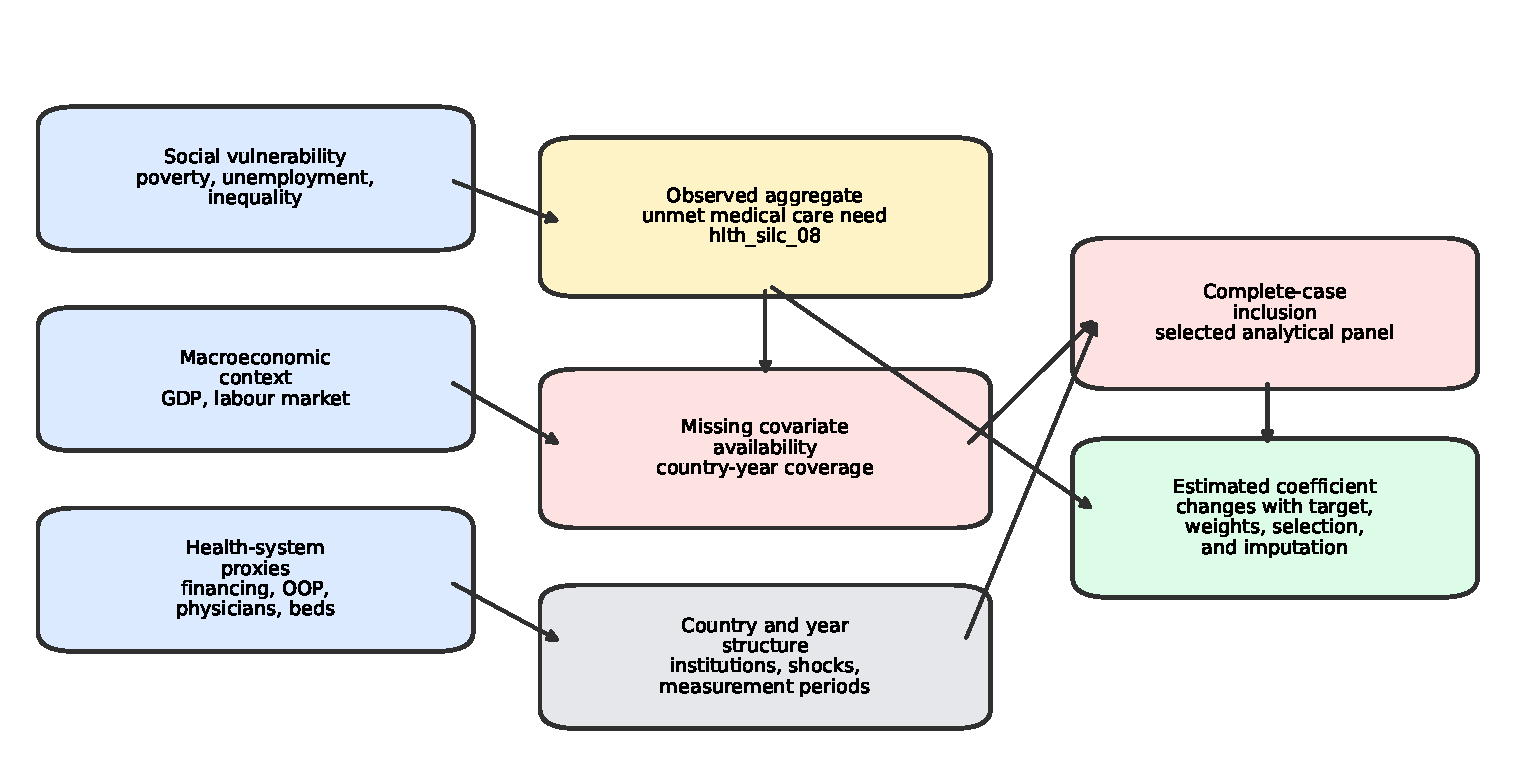
\includegraphics[width=0.92\textwidth]{conceptual_selection_estimand_diagram}
\caption{Conceptual selection and estimand diagram for the aggregate Eurostat design. The figure is not a causal DAG. It shows how access-domain covariates, country/year structure, missing covariate availability, and complete-case inclusion jointly determine which monitoring estimand is being estimated.}
\label{fig:conceptual_selection_estimand_diagram}
\end{figure}

Figure~\ref{fig:conceptual_selection_estimand_diagram} gives the chapter's organising logic. Social vulnerability, macroeconomic context, and health-system proxies are related to the observed aggregate outcome, but missing covariate availability also determines whether a country-year enters the complete-case regression. Missingness is therefore part of the estimand, not only a nuisance.

\section{Measurement of Self-Reported Unmet Care}

Eurostat's EU-SILC health metadata state that the health component contains health-status variables and unmet-needs variables for medical and dental care \citep{eurostat_health_variables_metadata}. The unmet-needs variables refer to a respondent's own assessment of whether they needed a specific type of examination or treatment but did not have it or did not seek it \citep{eurostat_health_variables_silc_methodology}. Medical care excludes dental care and refers to medical examination or treatment provided by, or under the supervision of, medical doctors or equivalent professions \citep{eurostat_health_variables_silc_methodology}.

The source is harmonised but not mechanically identical to an administrative registry. Eurostat describes EU-SILC methodology as being defined through a legislative framework to support comparability across EU, EFTA, and candidate countries, with yearly methodological guidelines for implementation \citep{eurostat_eusilc_methodology}. At the same time, EU-SILC combines interview data, national survey implementation, administrative sources, and imputations in ways that require explicit documentation \citep{eurostat_silc_information_data}. The empirical design therefore treats the Eurostat table as a public monitoring source whose comparability is supported institutionally, while still requiring checks for coverage, denominator choice, and measurement-period changes.

The official health-variable methodology lists the main reasons for unmet need as categories including care being too expensive, waiting list, inability to take time because of work or care responsibilities, too far to travel or no transportation, fear, waiting to see whether the problem improved, not knowing a good doctor or dentist, and other reasons \citep{eurostat_health_variables_silc_methodology}. This thesis uses the Eurostat aggregate category that combines the access-barrier reasons most directly connected to system functioning: expense, distance, and waiting lists. These are substantively related, but they are not identical mechanisms.

The primary outcome, \texttt{hlth\_silc\_08}, is an all-population percentage of people aged 16 or over reporting unmet medical examination or treatment. Eurostat's unmet-healthcare article distinguishes this type of indicator from a second indicator expressed as a percentage of people who reported having a medical need \citep{eurostat_unmet_needs_statistics}. The robustness outcome, \texttt{hlth\_silc\_08b}, belongs to that second denominator family. It is therefore useful as a denominator check, but it is not an interchangeable replacement for \texttt{hlth\_silc\_08}.

This denominator distinction is analytically important. A population-denominator rate combines at least two components: whether people perceive or report a need and whether that need is unmet. A need-denominator rate focuses more narrowly on unmet access among people reporting need. \citet{A4_ramos_2019} argue that ordinary unmet-need measures can hide this difference, and \citet{ingleby_guidi_2025_unmet_needs_methodology} explain that the 2015 EU-SILC change made it possible to distinguish the probability of reporting need from the probability that care was not received. This is why the thesis treats \texttt{hlth\_silc\_08b} as measurement robustness over 2021--2025 rather than as a second main outcome.

EU-SILC is also a survey of private households and persons living in those households. Eurostat states that all household members are surveyed but only those aged 16 or older are interviewed, while people in collective households and institutions are generally outside the target population \citep{eurostat_silc_information_data, eurostat_income_living_metadata}. Health variables are collected through interviews rather than administrative records \citep{eurostat_health_variables_silc_methodology}. Consequently, self-reported unmet care should not be read as clinical need, administrative denial of service, or objective health-system quality. It is a harmonised monitoring indicator based on reported need, reported non-use, and reason categories.

The 2015 issue is handled as a measurement-period caution. The literature notes that a change in the EU-SILC health-needs questionnaire from 2015 onwards separated the need question from the unmet-care question, making need-denominator indicators possible \citep{ingleby_guidi_2025_unmet_needs_methodology}. In the present aggregate panel, the baseline complete-case regression starts in 2015 because covariate coverage is thin before that year. A formal complete-case pre/post-2015 split is therefore not available for the main poverty coefficient. Chapter~\ref{ch:modeling_strategy_results} uses excluding-2015 and 2016-onward checks, while descriptive pre/post patterns are interpreted cautiously.

\section{Individual-Level European Evidence}

Individual-level European studies consistently link unmet medical care need to social vulnerability. Lower income, unemployment, difficulty making ends meet, poor health, debt, and housing vulnerability are associated with higher access barriers in EU-SILC and related European survey evidence \citep{A1_chaupain_guillot_2015, A2_madureira_lima_2018, A3_israel_2016, A5_cylus_papanicolas_2015}. Studies of financing and protection show that out-of-pocket payments, social-policy design, and public pensions can matter for cost-related unmet need \citep{B2_kaminska_wulfgramm_2019, C4_reeves_mckee_mackenbach_2017}. Crisis-period work from Greece, Portugal, and the Baltic states links economic stress and health-system pressure to access problems \citep{zavras_zavras_kyriopoulos_2016, legido_quigley_karanikolos_2016, karanikolos_gordeev_mackenbach_2016}.

This evidence motivates the choice of poverty or social exclusion as the stress-test coefficient. It does not imply that the thesis estimates the individual-level social gradient. Microdata studies can observe household income, self-reported health, employment, education, citizenship, and personal characteristics. This thesis observes national averages. Agreement with microdata literature can make the aggregate poverty association substantively plausible, but it cannot convert a country-year coefficient into evidence about individual behaviour.

The same distinction applies to citizenship. European access studies often treat migration status, legal entitlement, language, and socioeconomic position as linked access dimensions. The aggregate Eurostat citizenship rows used in this thesis cannot adjust for income, health status, legal status, language, local service conditions, or duration of residence. They are therefore descriptive equity context, not a parallel contribution to individual-level access theory.

\section{Aggregate Monitoring and Ecological Inference}

Country-year panels are useful for monitoring because they make cross-national coverage, trends, and policy-relevant indicators visible. They are weak for mechanisms because the unit of analysis is the country-year rather than the person. Classic work on ecological correlations shows that aggregate relationships can differ from individual relationships \citep{robinson_1950}. Epidemiological work further shows that ecological bias can arise through aggregation, contextual confounding, compositional differences, and effect modification \citep{greenland_morgenstern_1989}.

This is not a minor caveat. Poverty, unemployment, citizenship, and unmet care operate through individual and household mechanisms, but this thesis observes only country-year summaries. A positive country-year poverty coefficient does not show that poorer individuals in a country forgo care. It may reflect compositional change, national policy context, reporting expectations, macroeconomic shocks, health-system pressure, or measurement coverage. For this reason, the estimand is explicitly an aggregate monitoring estimand.

The aggregate design is still defensible when the question is framed correctly. The thesis does not ask whether poverty causes an individual to report unmet need. It asks whether an aggregate Eurostat poverty association is stable when the analyst changes target population, weighting, row selection, and imputation assumptions. That is a methodological monitoring question rather than a micro-level access question.

\section{Missing Data, Complete Cases, and Estimand Drift}

Missingness is the central methodological problem because the outcome is observed for more country-years than the baseline covariates. Complete-case analysis can therefore change the target population. Missing-data theory distinguishes complete-case analysis, inverse-probability weighting, and multiple imputation under explicit assumptions \citep{rubin_1987, little_rubin_2019}. IPW can address missingness when observation probabilities are well modelled and positivity holds, but it cannot recover structurally absent covariates \citep{seaman_white_2013}.

In this thesis, estimand drift occurs when the analysis silently moves from the 608-row outcome-observed panel to the 282-row complete-case fixed-effects sample. That movement is not only a loss of power. It changes which countries and years define the coefficient. If excluded rows have different unmet need, GDP, unemployment, or poverty levels, then the complete-case coefficient belongs to a selected analytical panel rather than to the intended monitoring target.

Multiple imputation is used as a sensitivity design, not as a rescue operation. A MAR-type imputation model asks what happens if missing covariates can be predicted from observed variables, country or country-group structure, year structure, and the observed outcome. That assumption is not verifiable from the observed aggregate data. Structural Eurostat non-coverage, country-specific reporting practices, and variables that exist only over shorter windows may violate MAR. The MNAR delta-shift checks therefore ask whether the conclusion depends mechanically on one MAR imputation model.

The interpretation rule is deliberately conservative. If complete-case specifications remain positive but MAR and MNAR full-target imputation attenuate the coefficient, the thesis does not declare the imputed coefficient to be true. It concludes that the complete-case poverty association is estimand-dependent and model-dependent. This is the core contribution.

\section{Reporting Discipline for Observational Monitoring}

The thesis follows a STROBE-style reporting logic for observational data: data source, eligibility, variables, bias, statistical methods, missing data, and limitations are stated before interpreting model output \citep{von_elm_altman_egger_2007_strobe}. This matters because the project is not a controlled experiment and does not have a single natural denominator. The key reporting unit is therefore not only the regression coefficient, but also the target population, row-selection rule, country universe, weighting rule, covariance estimator, and missing-data assumption attached to each coefficient.

This reporting discipline is also why the thesis avoids treating robustness checks as interchangeable. Complete-case, population-weighted, balanced-outcome, IPW, MAR MI, and MNAR rows are different estimands or sensitivity targets. They do not form a simple tournament for the one correct answer. Their value is to reveal where the interpretation changes.

\section{Panel Dependence and Prediction Validation}

Panel inference requires dependence-aware uncertainty because each country contributes repeated observations. Cluster-robust inference for within estimators is standard when errors may be correlated within countries \citep{arellano_1987}. The panel literature also warns that serial correlation can lead to overconfident inference if repeated observations are treated as independent \citep{bertrand_duflo_mullainathan_2004}. For this reason, the thesis reports country-clustered standard errors for pooled and two-way fixed-effects models, with Driscoll--Kraay and wild-cluster bootstrap diagnostics added for the main selected-panel coefficient.

Prediction is secondary but must still respect the panel structure. Country-year data have temporal dependence and strong country persistence, so random row splits overstate generalisation. Structured validation is recommended when observations are temporally, spatially, or hierarchically dependent \citep{roberts_2017_cross_validation}. Recent prediction-model reporting and bias-assessment guidance reinforces the same principle: the target population, outcome, predictors, validation design, performance uncertainty, and risk of bias must be transparent \citep{collins_moons_dhiman_2024_tripod_ai, moons_damen_kaul_2025_probast_ai}. In this thesis those standards are used only to discipline the benchmark exercise, not to claim a clinical prediction-model contribution.

The thesis therefore defines prediction as one-year-ahead benchmarking using lagged predictors. Same-year prediction is closer to nowcasting and is not treated as the main predictive claim. Flexible machine-learning models are benchmark competitors, not a separate scientific contribution. Feature importance is model inspection only, because tree-model impurity importance can be biased by scale, variation, and split opportunities \citep{strobl_boulesteix_zeileis_hothorn_2007_bias}.

\chapter{Data and Indicators}
\label{ch:data_indicators}

\section{Data Source and Unit of Analysis}

The thesis uses published aggregate Eurostat data. The unit of analysis is the country-year, so each row represents one national observation in one calendar year. This design differs from an EU-SILC microdata study: it cannot observe individuals, households, health status, income quintiles, or local service conditions directly. Its value is that it provides a reproducible panel of national indicators that can be used for descriptive comparison, regression analysis, and prediction.

The data construction follows a national-only scope. EU and euro-area aggregate codes are excluded from the modelling data, and regional NUTS2 sources are not used in the core analysis. The dataset audit found that regional dataflows exist, but a clean balanced regional panel was not verified. The national design is therefore more conservative and more consistent with the aim of producing a reproducible MSc thesis from open Eurostat sources.

The empirical design starts from a public-data estimand registry rather than from a single outcome file. Table~\ref{tab:public_data_estimand_registry} lists the feasible core unmet-care indicators extracted for the multi-outcome benchmark. It includes medical and dental care, population-denominator and need-denominator definitions, and medical barrier-specific indicators for cost, distance, and waiting lists. Eurostat reason codes are verified programmatically from the downloaded JSON-stat metadata; indicators that cannot be verified are retained in the registry with an infeasibility reason instead of being silently dropped.

\begin{table}[htbp]
\centering
\scriptsize
\caption{Public-data estimand registry for feasible Eurostat unmet-care indicators. The registry defines the outcome object before modelling: dataset, care type, barrier definition, denominator, observed years, country count, row count, and feasibility status.}
\label{tab:public_data_estimand_registry}
\begingroup
\scriptsize
\setlength{\tabcolsep}{3pt}
\begin{tabularx}{\linewidth}{@{}p{0.21\linewidth}p{0.13\linewidth}Yp{0.11\linewidth}p{0.12\linewidth}rrp{0.09\linewidth}@{}}
\toprule
Indicator & Dataset & Barrier & Denom. & Years & Countries & Rows & Status \\
\midrule
Medical population & hlth\_silc\_08 & Cost, distance, waiting & Population & 2008--2025 & 37 & 608 & feasible \\
Medical need & hlth\_silc\_08b & Cost, distance, waiting & Need & 2021--2025 & 34 & 154 & feasible \\
Dental population & hlth\_silc\_09 & Cost, distance, waiting & Population & 2008--2025 & 37 & 607 & feasible \\
Dental need & hlth\_silc\_09b & Cost, distance, waiting & Need & 2021--2025 & 34 & 154 & feasible \\
Medical cost & hlth\_silc\_08 & Cost & Population & 2008--2025 & 37 & 608 & feasible \\
Medical waiting & hlth\_silc\_08 & Waiting & Population & 2008--2025 & 37 & 608 & feasible \\
Medical distance & hlth\_silc\_08 & Distance & Population & 2008--2025 & 37 & 608 & feasible \\
\bottomrule
\end{tabularx}
\endgroup

\end{table}

The term ``Europe'' is used operationally rather than institutionally. The full Eurostat-available universe means all national units that appear in the selected Eurostat outcome and covariate tables after excluding EU and euro-area aggregates. For sensitivity analysis, the thesis distinguishes EU-27 member states from EEA countries, Switzerland, the UK, EU candidate or potential-candidate countries, and any other Eurostat-available national units. Table~\ref{tab:country_universe} reports how these country groups enter the outcome-observed panel, complete-case fixed-effects sample, MI target, and prediction sample.

\begin{table}[htbp]
\centering
\scriptsize
\caption{Country universe and sample inclusion. The table defines the operational country universe used in the thesis and reports inclusion in the outcome-observed panel, complete-case FE sample, MI target, and ML sample.}
\label{tab:country_universe}
\resizebox{\textwidth}{!}{%
\begin{tabular}{@{}llrrrr@{}}
\toprule
Country & Universe category & Outcome rows & CC rows & MI rows & ML rows \\
\midrule
AL & Candidate/potential candidate & 7 & 0 & 7 & 0 \\
AT & EU-27 & 18 & 10 & 18 & 9 \\
BE & EU-27 & 18 & 9 & 18 & 9 \\
BG & EU-27 & 18 & 9 & 18 & 9 \\
CH & Switzerland & 17 & 10 & 17 & 9 \\
CY & EU-27 & 18 & 9 & 18 & 9 \\
CZ & EU-27 & 18 & 10 & 18 & 5 \\
DE & EU-27 & 18 & 10 & 18 & 9 \\
DK & EU-27 & 18 & 10 & 18 & 8 \\
EE & EU-27 & 18 & 10 & 18 & 9 \\
EL & EU-27 & 18 & 9 & 18 & 0 \\
ES & EU-27 & 18 & 9 & 18 & 9 \\
FI & EU-27 & 18 & 9 & 18 & 9 \\
FR & EU-27 & 18 & 10 & 18 & 9 \\
HR & EU-27 & 16 & 9 & 16 & 9 \\
HU & EU-27 & 18 & 10 & 18 & 9 \\
IE & EU-27 & 18 & 10 & 18 & 9 \\
IS & EEA country & 13 & 6 & 13 & 4 \\
IT & EU-27 & 17 & 9 & 17 & 8 \\
LT & EU-27 & 18 & 10 & 18 & 9 \\
LU & EU-27 & 18 & 10 & 18 & 9 \\
LV & EU-27 & 18 & 9 & 18 & 9 \\
ME & Candidate/potential candidate & 11 & 0 & 11 & 0 \\
MK & Candidate/potential candidate & 15 & 0 & 15 & 0 \\
MT & EU-27 & 18 & 9 & 18 & 9 \\
NL & EU-27 & 18 & 10 & 18 & 9 \\
NO & EEA country & 18 & 8 & 18 & 8 \\
PL & EU-27 & 18 & 10 & 18 & 9 \\
PT & EU-27 & 18 & 10 & 18 & 0 \\
RO & EU-27 & 18 & 9 & 18 & 9 \\
RS & Candidate/potential candidate & 13 & 0 & 13 & 0 \\
SE & EU-27 & 18 & 10 & 18 & 8 \\
SI & EU-27 & 18 & 10 & 18 & 9 \\
SK & EU-27 & 18 & 9 & 18 & 0 \\
TR & Candidate/potential candidate & 18 & 0 & 18 & 0 \\
UK & UK & 11 & 0 & 11 & 0 \\
XK & Candidate/potential candidate & 2 & 0 & 2 & 0 \\
\bottomrule
\end{tabular}%
}

\vspace{0.2em}
\begin{minipage}{0.96\textwidth}\scriptsize Notes: Country universe categories distinguish EU-27 members, EEA countries, Switzerland, the UK, candidate or potential-candidate countries, and other Eurostat-available national units. CC rows are baseline complete-case fixed-effects rows; MI rows are outcome-observed target rows.\end{minipage}

\end{table}

All indicators are merged by country and year. The primary panel is built around the availability of the main outcome, and covariates are added using exact Eurostat dataset codes and filters. Missingness is then handled in the modelling chapters through complete-case samples and sensitivity checks. This means that descriptive analysis, regression, and machine-learning models do not always use the same set of country-year observations.

\section{Primary Outcome}

The primary outcome is \texttt{hlth\_silc\_08}, the Eurostat EU-SILC indicator for self-reported unmet needs for medical examination by sex, age, main reason declared, and income quintile \citep{eurostat_health_variables_metadata, eurostat_unmet_needs_statistics}. The thesis uses the aggregate filter for total sex, persons aged 16 and over, total income quantile, and unmet medical care need due to expense, distance, or waiting lists. The resulting variable is named \texttt{unmet\_need\_pc}.

This outcome is appropriate because it directly matches the thesis topic and is available as a harmonised Eurostat country-level series. It measures a reported access problem, not a clinical diagnosis and not a direct measure of health-system quality. Respondents must perceive a medical need, report that the need was not met, and classify the reason through the survey categories. This is a known comparability challenge for self-reported access indicators \citep{guidi_ingleby_2023_valid_data}. For this reason, all interpretations remain associational and descriptive.

The primary outcome is also broader than a need-denominator measure. It is expressed as a share of the relevant population rather than only among persons who report having the same medical needs. This distinction matters because a national rate may reflect both the prevalence of need and the probability that need remains unmet. Chapter~\ref{ch:background_literature} discusses this measurement issue, and the robustness outcome below is used to check the denominator distinction.

\section{Covariate Blocks}

The covariates are grouped into macroeconomic, labour-market, inequality, health-financing, and health-capacity blocks. Table~\ref{tab:variable_summary} summarises the main variables and selected engineered features. The list is limited to indicators with verified Eurostat sources and a plausible connection to unmet medical care need. The aim is not to build a complete theory of healthcare access, but to represent the main country-year conditions that the literature identifies as relevant.

\begin{table}[htbp]
\centering
\scriptsize
\caption{Summary of primary variables and selected engineered features. The table lists Eurostat country-year variables used in the national aggregate panel; availability varies by source and year.}
\label{tab:variable_summary}
\begingroup
\setlength{\tabcolsep}{4pt}
\begin{tabular}{@{}>{\raggedright\arraybackslash}p{0.22\textwidth}>{\raggedright\arraybackslash}p{0.38\textwidth}>{\raggedright\arraybackslash}p{0.23\textwidth}r@{}}
\toprule
Variable & Description & Source & Years \\
\midrule
\path{unmet_need_pc} & Primary outcome: unmet medical examination need due to cost, distance, or waiting list; persons aged 16+. & Eurostat \texttt{hlth\_silc\_08} & 2008--2025 \\
\path{unmet_need_pc_08b} & Robustness outcome: same access-barrier reasons, measured among persons having the same medical needs. & Eurostat \texttt{hlth\_silc\_08b} & 2021--2025 \\
\path{gdp_per_capita_eur} & Macroeconomic level: current-price GDP per inhabitant. & Eurostat \path{nama_10_pc} & 2008--2025 \\
\path{unemployment_rate_pc} & Labour-market condition: unemployment rate for ages 15--74. & Eurostat \path{une_rt_a} & 2008--2025 \\
\path{poverty_or_social_exclusion_pc} & Inequality and poverty: persons at risk of poverty or social exclusion. & Eurostat \path{ilc_peps01n} & 2015--2025 \\
\path{government_health_expenditure_gdp_pc} & Health-system financing: general government health expenditure as share of GDP. & Eurostat \path{gov_10a_exp} & 2008--2025 \\
\path{compulsory_health_financing_gdp_pc} & Health-system financing: compulsory financing schemes as share of GDP. & Eurostat \path{hlth_sha11_hf} & 2008--2024 \\
\path{physicians_per_100k} & Health-system capacity: practising physicians per 100,000 inhabitants. & Eurostat \path{hlth_rs_prs2} & 2008--2024 \\
\path{hospital_beds_per_100k} & Health-system capacity: total hospital beds per 100,000 inhabitants. & Eurostat \path{hlth_rs_bds1} & 2008--2024 \\
\path{oop_health_expenditure_share_pc} & Health-system financing: out-of-pocket spending as share of current health expenditure. & Eurostat \path{hlth_sha11_hf} & 2008--2024 \\
\path{gini_income} & Inequality: Gini coefficient of equivalised disposable income. & Eurostat \path{ilc_di12} & 2014--2025 \\
\path{long_term_unemployment_rate_pc} & Labour-market condition: long-term unemployment rate for ages 15--74. & Eurostat \path{une_ltu_a} & 2008--2025 \\
\path{log_gdp_per_capita} & Engineered feature: natural log of GDP per inhabitant. & Derived: \texttt{nama\_10\_pc} & 2008--2025 \\
\path{gdp_per_capita_growth} & Engineered feature: annual within-country change in GDP per inhabitant. & Derived: \texttt{nama\_10\_pc} & 2009--2025 \\
\path{unemployment_rate_change} & Engineered feature: annual within-country change in unemployment rate. & Derived: \texttt{une\_rt\_a} & 2009--2025 \\
\path{physicians_per_100k_lag1} & Engineered feature: one-year lag of practising physicians per 100,000 inhabitants. & Derived: \texttt{hlth\_rs\_prs2} & 2009--2025 \\
\bottomrule
\end{tabular}
\endgroup

\end{table}

The macroeconomic block is based on GDP per capita. This indicator is used as a broad measure of national economic resources and living standards. The thesis also uses a logged GDP feature and a within-country GDP growth feature in the predictive modelling dataset. These transformations help represent proportional differences and changes over time, but they do not turn GDP into a causal variable.

The labour-market block includes the unemployment rate and long-term unemployment rate. These variables are included because labour-market pressure can be associated with financial insecurity, weaker household buffers, and social vulnerability. The feature set also contains an unemployment-rate change variable, which captures within-country annual movement. This is a descriptive change measure and is not interpreted as a shock design.

The inequality and poverty block includes poverty or social exclusion and the Gini coefficient of equivalised disposable income. Poverty or social exclusion is central to the thesis hierarchy because it is the clearest social vulnerability indicator in the regression analysis. The Gini coefficient adds an income-distribution perspective, which is useful because national average income and poverty rates do not describe the same social structure.

The health-financing block includes government health expenditure, compulsory health financing, and out-of-pocket expenditure. These variables are close to the outcome concept because cost is one of the reported reasons for unmet medical care need. They are nevertheless interpreted cautiously. Higher public spending may reflect capacity or protection, but it may also reflect need, prices, or policy response. Out-of-pocket spending may indicate burden, but it can also reflect private-sector use by groups able to pay.

The health-capacity block includes physicians per 100,000 inhabitants and hospital beds per 100,000 inhabitants. These are national averages, so they cannot capture geographic distribution, specialty shortages, or local waiting-time conditions. They are included because capacity may still be predictive of unmet medical care need, especially where the reported barrier is waiting time or distance. A lagged physician-density feature is also used in the machine-learning feature set.

\section{Engineered Features}

The feature-engineering step creates logged, lagged, and change variables within country. Logged variables reduce the influence of very large country differences, while change variables describe year-to-year movement. Lag variables are included because some country-year conditions may be more plausibly related to access with delay than only contemporaneously. These features remain predictive covariates, not causal instruments.

No values are carried forward to fill missing covariates during feature engineering. This choice keeps the data construction transparent and avoids silently creating artificial observations. The cost is that lag and change variables mechanically reduce the available complete-case sample. The modelling chapters therefore report complete-case results and sensitivity checks rather than claiming full coverage of all observed outcome rows.

\section{Population Weights and Target Populations}

The revised thesis adds Eurostat \texttt{demo\_pjan} total population by country-year. The extraction uses total sex, total age, annual frequency, and number of persons. The outcome-observed panel covers 2008--2025, while the baseline complete-case fixed-effects model covers 2015--2024 because baseline covariate coverage begins later and is incomplete in 2025.

The unweighted descriptive estimand is an average-country-year quantity over the observed outcome set \(O\):
\[
\mu_{O} = \frac{1}{|O|}\sum_{(i,t)\in O} y_{it},
\]
where \(y_{it}\) is unmet medical care need in country \(i\) and year \(t\). This estimand treats each observed country-year equally.

Population-weighted estimates use country-year populations normalized within each year:
\[
w_{it} = \frac{N_{it}}{\sum_{j \in O_t} N_{jt}},
\]
where \(N_{it}\) is country \(i\)'s population in year \(t\), and \(O_t\) is the set of observed countries in that year. Each year therefore contributes equally, while larger countries receive greater weight within year. This defines an average-European-resident monitoring estimand.

For a regression coefficient, the complete-case estimand is conditional on the observed covariate-complete set \(C\):
\[
\beta_{CC} \text{ is estimated from } \{(i,t): y_{it},X_{it}\ \text{are observed for all baseline covariates}\}.
\]
The population-weighted complete-case estimand uses the same set \(C\) but applies \(w_{it}\). The MI full-target estimand keeps the broader outcome-observed set \(O\) and replaces missing covariates with draws from the imputation model:
\[
\beta_{MI} = \frac{1}{M}\sum_{m=1}^{M}\hat{\beta}^{(m)}_{O},
\]
with uncertainty pooled using Rubin's rules. This notation is a reminder that MI changes the target and adds model dependence; it does not establish a target-invariant coefficient.

The planned MNAR sensitivity estimand keeps the same outcome-observed set \(O\) but applies explicit departures from the MAR imputation model:
\[
\beta_{MNAR(\delta)} = \frac{1}{M}\sum_{m=1}^{M}\hat{\beta}^{(m)}_{O,\delta},
\]
where \(\delta\) denotes a documented shift to imputed values for missing poverty, GDP, or unemployment. This estimand is a stress test for imputation assumptions, not a corrected estimate.

Population weighting is not treated as more correct than unweighted analysis. The unweighted panel answers an average-country monitoring question, while the weighted panel answers an average-resident monitoring question. The balanced-outcome panel is also defined at this stage: it includes countries with complete primary-outcome coverage and valid population weights over the main analysis window. It is not automatically balanced for every regression covariate.

\begin{figure}[htbp]
\centering
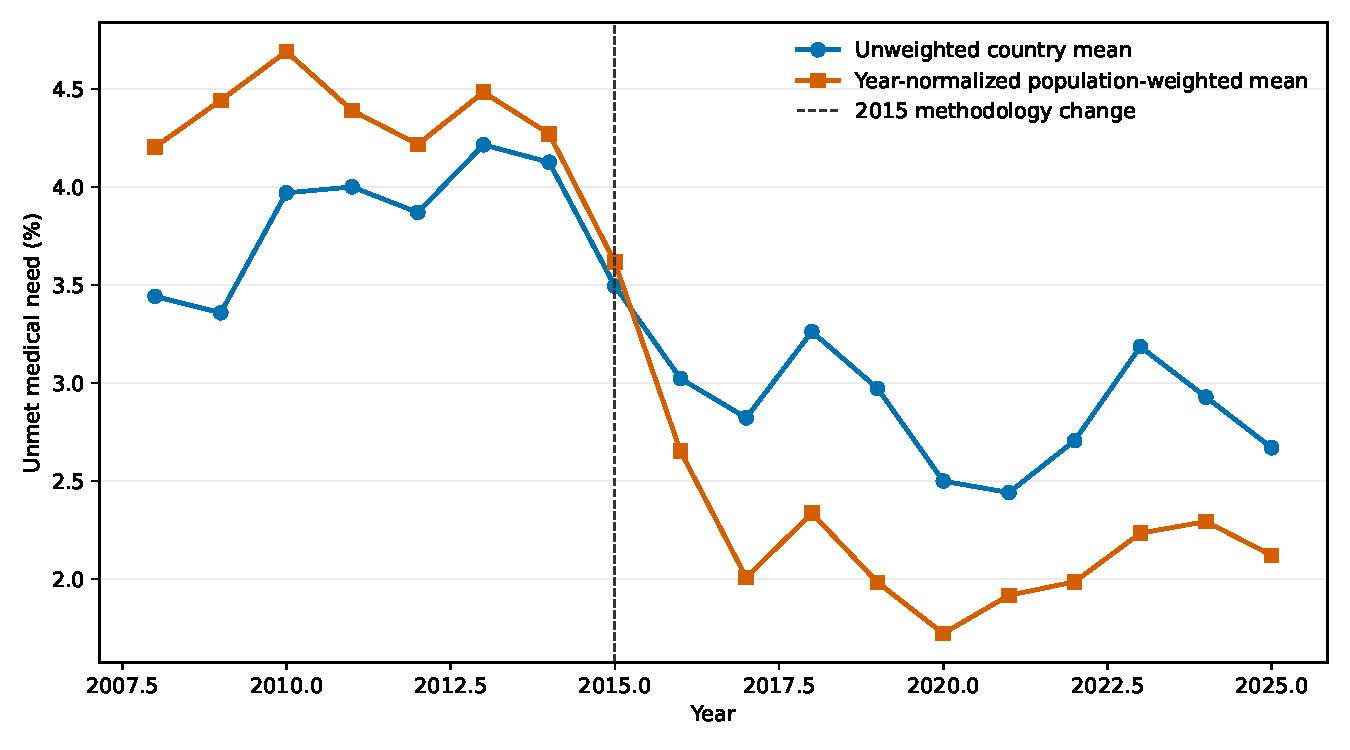
\includegraphics[width=0.86\textwidth]{population_weighted_trend}
\caption{Unweighted and year-normalized population-weighted trends in unmet medical care need. The sample is observed \texttt{hlth\_silc\_08} country-years over 2008--2025; country coverage can vary by year, and population weights use \texttt{demo\_pjan} normalized within year.}
\label{fig:population_weighted_trend}
\end{figure}

\section{Missingness and Sample Construction}

Missingness is a substantive part of the empirical design. Some Eurostat indicators have shorter time coverage than \texttt{hlth\_silc\_08}, and some are unavailable for specific countries. Chapter~\ref{ch:descriptive_evidence} shows the grouped missingness heatmaps used to diagnose this coverage pattern. They are data-quality and sample-construction diagnostics, not substantive results by themselves.

The regression sample is complete-case. The baseline two-way FE model uses \(N=282\) country-year observations, as reported in the regression output summary. This restriction is necessary because all selected covariates must be observed in the same country-year row. It also means that the regression results describe the available complete-case panel rather than every European country-year observed in the outcome file.

The 2015 marker used in descriptive figures is not treated as a formal regression discontinuity. Because the baseline complete-case regression starts in 2015, the thesis cannot estimate a valid complete-case pre/post-2015 split for the poverty coefficient. Instead, Chapter~\ref{ch:modeling_strategy_results} reports excluding-2015 and 2016-onward diagnostics, while the descriptive chapter treats pre/post-2015 outcome patterns cautiously.

Table~\ref{tab:missingness_comparison} compares rows included in the baseline regression sample with rows excluded because of missing covariates. The excluded rows have higher unmet medical care need and lower GDP on average. This is an important limitation because complete-case attrition is not random with respect to the outcome and economic context. The thesis therefore treats missingness as part of the interpretation of all regression and prediction results.

\begin{table}[htbp]
\centering
\small
\caption{Included and excluded country-year rows in the baseline regression sample. The comparison uses the 608 outcome-observed country-years and contrasts the 282-row complete-case FE sample with rows excluded by missing baseline covariates.}
\label{tab:missingness_comparison}
\begingroup
\small
\begin{tabular}{@{}lrrrrrr@{}}
\toprule
Variable & Inc. \(N\) & Inc. mean & Exc. \(N\) & Exc. mean & Diff. & p-value \\
\midrule
Unmet need & 282 & 2.63 & 326 & 3.85 & -1.23 & <0.001 \\
GDP/cap. & 282 & 36851.38 & 322 & 26235.31 & 10616.07 & <0.001 \\
Unemp. & 282 & 6.86 & 274 & 10.48 & -3.62 & <0.001 \\
Poverty & 282 & 21.00 & 93 & 28.39 & -7.39 & <0.001 \\
\bottomrule
\end{tabular}

\vspace{0.2em}
\begin{minipage}{0.92\textwidth}\scriptsize Notes: Welch tests compare rows included in the baseline complete-case regression with outcome-observed rows excluded because at least one baseline covariate is missing. The table is descriptive and is used as a selection diagnostic.\end{minipage}
\endgroup

\end{table}

\section{Robustness Outcome: \texttt{hlth\_silc\_08b}}

The robustness outcome is \texttt{hlth\_silc\_08b}. This Eurostat EU-SILC indicator measures unmet medical care need due to financial reasons, waiting lists, or distance among persons having the same needs \citep{eurostat_health_variables_metadata}. It is therefore close to the primary outcome in access-barrier content, but different in denominator. The thesis uses it as a robustness and interpretation check.

The key distinction is that \texttt{hlth\_silc\_08} is a broad population percentage, while \texttt{hlth\_silc\_08b} is a percentage among persons with the same medical needs. A higher value in \texttt{hlth\_silc\_08b} should not be read as a contradiction. It can arise because the denominator is narrower and more directly tied to reported need. This is why the robustness analysis does not replace the primary outcome.

\begin{table}[htbp]
\centering
\caption{Robustness comparison using \texttt{hlth\_silc\_08b}. The table is restricted to overlapping 2021--2025 country-year cells with complete shared controls and is a denominator check, not an alternative main outcome.}
\label{tab:robustness_08b_results}
\begin{tabular}{lcc}
\toprule
Variable & Primary outcome & Robustness outcome \\
\midrule
Log GDP per capita & -0.329 (0.234) & -0.443 (0.381) \\
Unemployment rate & 0.315 (0.100) & 0.550 (0.166) \\
Poverty or social exclusion & -0.004 (0.044) & 0.007 (0.068) \\
\midrule
Observations & 147 & 147 \\
Outcome table & \texttt{hlth\_silc\_08} & \texttt{hlth\_silc\_08b} \\
\bottomrule
\end{tabular}

\vspace{0.2em}
\begin{minipage}{0.82\textwidth}
\scriptsize Notes: Cells report coefficient estimates with standard errors in parentheses. The comparison is restricted to overlapping 2021--2025 country-year cells with complete values for the three shared controls. No star thresholds are used because this is a denominator sensitivity check, not a main inferential model.
\end{minipage}

\end{table}

Table~\ref{tab:robustness_08b_results} reports the compact robustness comparison. The purpose is to check whether the broad sign pattern is sensitive to using the need-denominator outcome for the overlapping period and shared controls. The table is not treated as a new core model because the verified period for \texttt{hlth\_silc\_08b} is shorter and the interpretation differs from the primary population-level measure.

\section{Scope Exclusions}

Several possible data extensions are excluded from the core thesis. EU-SILC microdata are not used because the project is based on public aggregate Eurostat data. EHIS indicators are not pooled with EU-SILC indicators because their wording, denominator, survey context, and population structure differ. Dental-care indicators are included in the estimand registry and monitoring benchmark as a separate service category, but they are not merged into the primary medical-care regression target. Dental reason-specific indicators remain optional unless extraction and coverage are clean enough to support a defensible benchmark.

ISTAT data are not merged into the core panel because no Eurostat-compatible Italian source with a verified extraction path was established for the thesis design. Regional NUTS2 data are also excluded because the audit did not verify a clean regional panel. These exclusions reduce scope, but they protect comparability. The final design is therefore a national aggregate Eurostat panel centred on \texttt{hlth\_silc\_08}, supported by \texttt{hlth\_silc\_08b} as a measurement robustness check.

\chapter{Multi-Outcome Monitoring Benchmark}
\label{ch:descriptive_evidence}

\section{Purpose}

This chapter is monitoring before modelling. It asks whether Eurostat unmet-care conclusions change before any association coefficient is estimated. The chapter therefore compares outcome definitions, denominators, country universes, and population-weighting rules in the public country-year panel. No regression coefficient is interpreted in this chapter.

The monitoring benchmark is the first layer of the target-population drift audit. It compares medical and dental indicators, population-denominator and need-denominator indicators, cost, waiting, and distance barriers, the full Eurostat-available country universe, the EU-27 restriction, and year-normalized population weighting. The primary medical indicator remains the detailed example because it has 608 observed country-years over 2008--2025, but it is no longer the only outcome object in the thesis.

\section{Multi-Outcome Monitoring Benchmark}

Figure~\ref{fig:multi_outcome_monitoring_benchmark} summarizes the benchmark. Panel A compares medical and dental unmet-care indicators using the population denominator. Panel B compares population-denominator and need-denominator definitions. Panel C separates medical cost, waiting-list, and distance barriers. Panel D shows how the primary medical indicator changes when the universe is restricted to EU-27 countries and when year-normalized population weights are applied.

\begin{figure}[htbp]
\centering
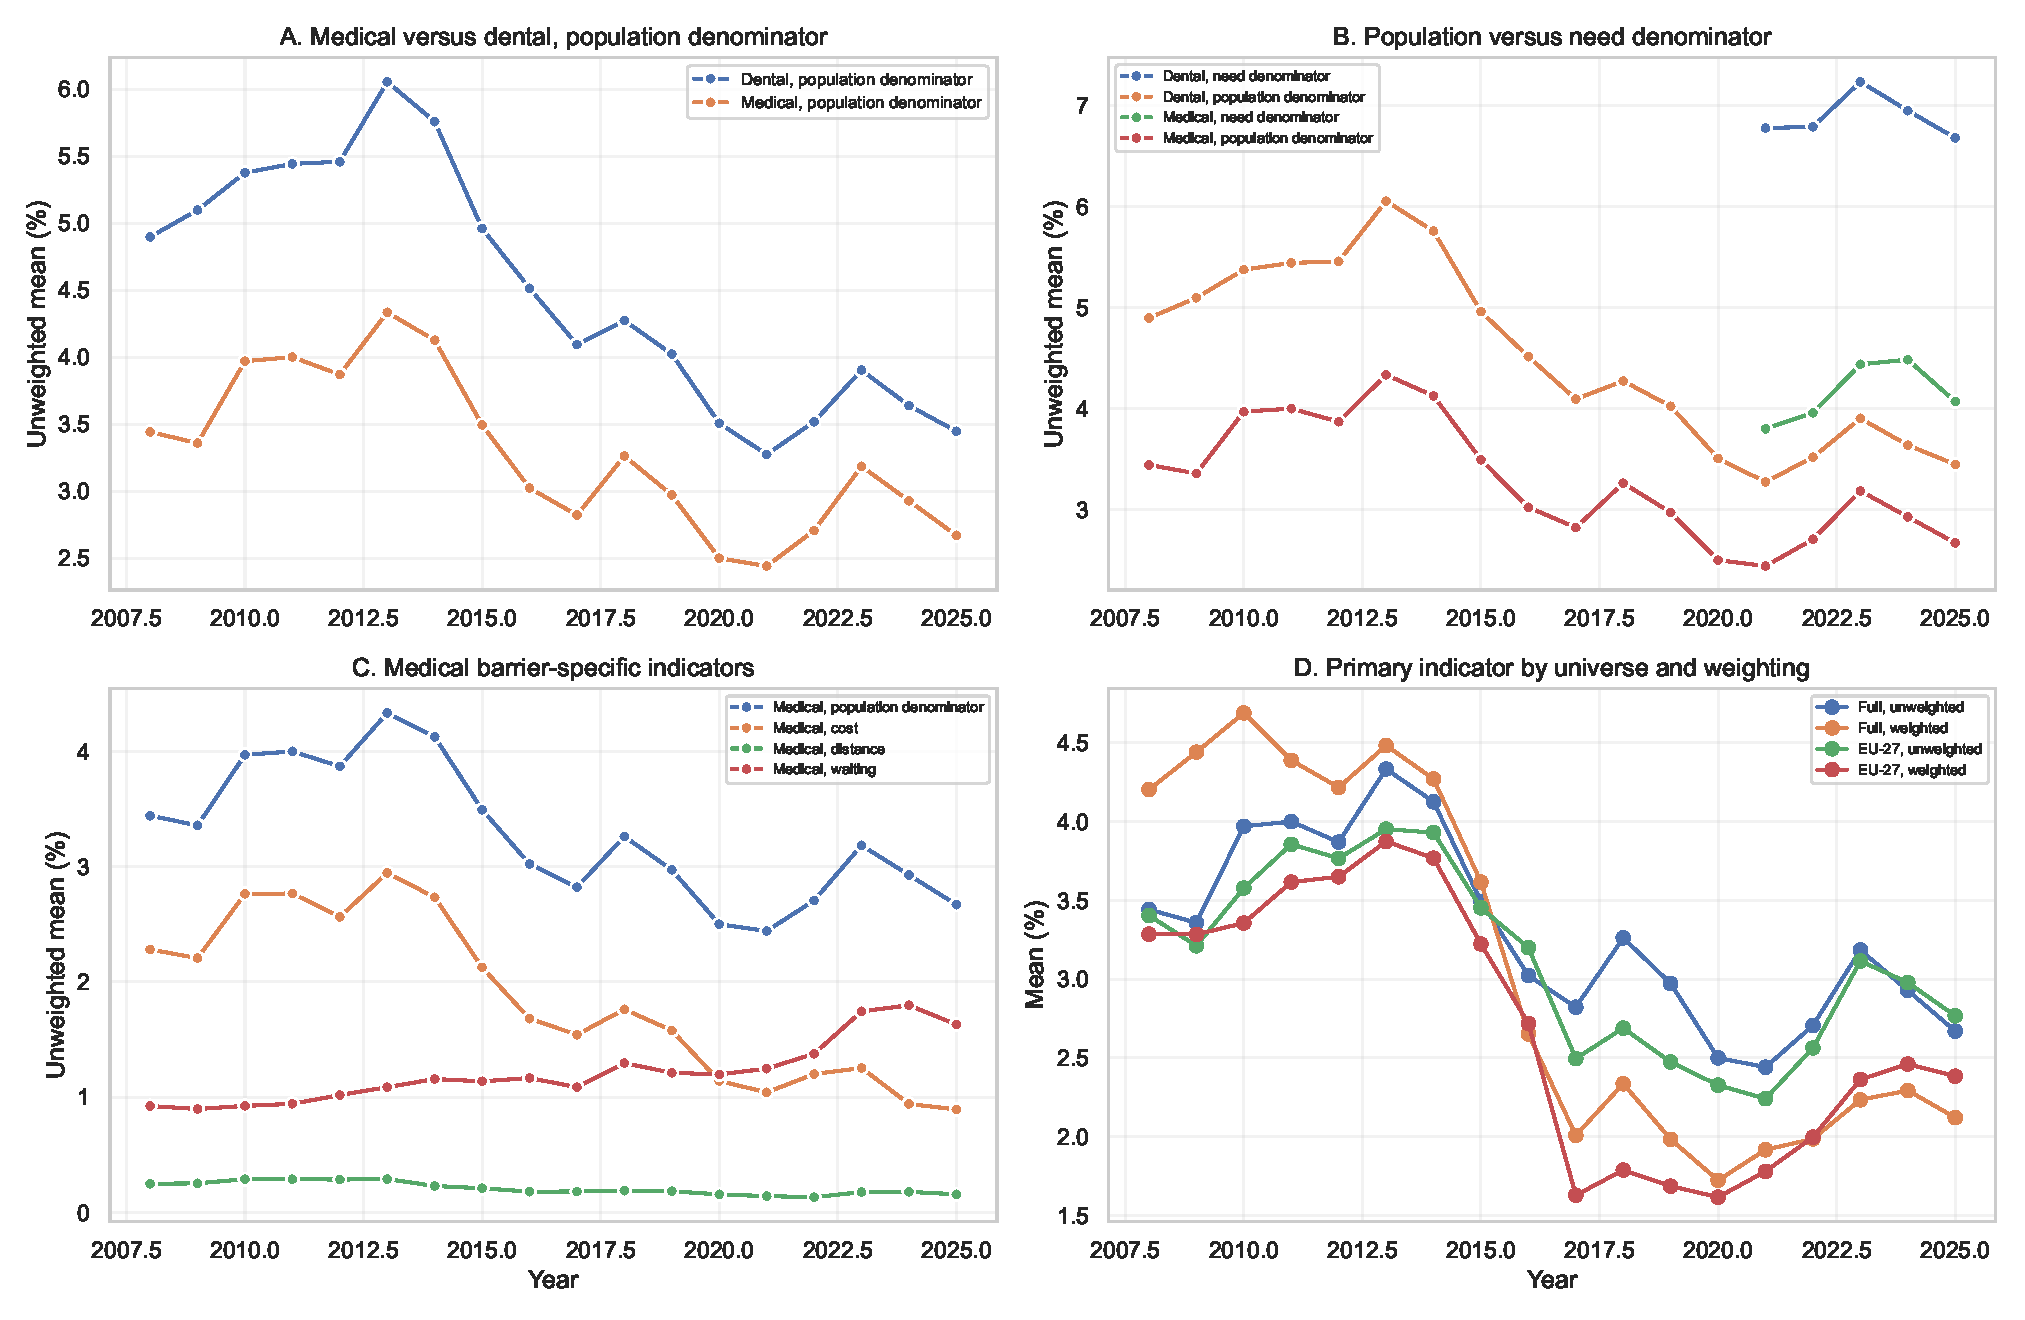
\includegraphics[width=0.98\textwidth]{multi_outcome_monitoring_benchmark}
\caption{Multi-outcome Eurostat unmet-care monitoring benchmark. The sample is national Eurostat country-year observations from the feasible indicators in Table~\ref{tab:public_data_estimand_registry}; population-denominator indicators cover 2008--2025 where available, need-denominator indicators cover 2021--2025, and country coverage varies by indicator and year. Weighted series use \texttt{demo\_pjan} populations normalized within each year and outcome.}
\label{fig:multi_outcome_monitoring_benchmark}
\end{figure}

The figure shows that monitoring conclusions are indicator-dependent before modelling begins. Medical and dental unmet care do not describe the same service domain. Population-denominator and need-denominator indicators answer different questions. Barrier-specific indicators separate affordability, waiting-time, and distance mechanisms. Population weighting changes the estimand from an average-country quantity to an average-resident quantity within each year.

\begin{table}[htbp]
\centering
\scriptsize
\caption{Coverage of feasible multi-outcome Eurostat unmet-care indicators. The table uses the full Eurostat-available national universe after excluding EU and euro-area aggregate codes; population rows count observations with valid \texttt{demo\_pjan} population available for year-normalized weighting.}
\label{tab:multi_outcome_coverage_table}
\begingroup
\setlength{\tabcolsep}{4pt}
\renewcommand{\arraystretch}{1.12}
\begin{tabularx}{\textwidth}{@{}Yllrrrr@{}}
\toprule
Indicator & Dataset & Denom. & Countries & Rows & Pop. rows & Years \\
\midrule
Dental, population denominator & hlth\_silc\_09 & population & 37 & 607 & 606 & 2008--2025 \\
Dental, need denominator & hlth\_silc\_09b & same\_needs & 34 & 154 & 154 & 2021--2025 \\
Medical, cost & hlth\_silc\_08 & population & 37 & 608 & 607 & 2008--2025 \\
Medical, population denominator & hlth\_silc\_08 & population & 37 & 608 & 607 & 2008--2025 \\
Medical, distance & hlth\_silc\_08 & population & 37 & 608 & 607 & 2008--2025 \\
Medical, waiting & hlth\_silc\_08 & population & 37 & 608 & 607 & 2008--2025 \\
Medical, need denominator & hlth\_silc\_08b & same\_needs & 34 & 154 & 154 & 2021--2025 \\
\bottomrule
\end{tabularx}
\endgroup

\end{table}

Table~\ref{tab:multi_outcome_coverage_table} gives the coverage behind the monitoring benchmark. The population-denominator medical and dental indicators provide long panels, while need-denominator indicators are shorter. This is not a defect to hide; it is an estimand fact that must be reported before comparisons are interpreted.

\begin{table}[htbp]
\centering
\scriptsize
\caption{Monitoring-dependence summary for 2025. Values are unweighted country means unless the comparison explicitly uses year-normalized population weighting; the table is descriptive and does not estimate any association model.}
\label{tab:multi_outcome_monitoring_dependence_summary}
\begingroup
\setlength{\tabcolsep}{4pt}
\renewcommand{\arraystretch}{1.14}
\begin{tabularx}{\textwidth}{@{}YrrrrY@{}}
\toprule
Comparison & Year & A & B & Diff. & Interpretation \\
\midrule
Unweighted versus resident-weighted primary indicator & 2025 & 2.67 & 2.121 & -0.549 & Population weighting changes the monitoring estimand from average country to average resident. \\
Full Eurostat-available versus EU-27 primary indicator & 2025 & 2.67 & 2.767 & 0.097 & Country-universe restriction changes the set of national units being summarized. \\
Medical population denominator versus medical need denominator & 2025 & 2.67 & 4.07 & 1.4 & Need-denominator indicators answer a narrower question than population-denominator indicators. \\
Medical versus dental population-denominator combined barriers & 2025 & 2.67 & 3.447 & 0.777 & Care type changes the service domain and should not be treated as the same outcome. \\
Medical barrier range: cost, waiting, distance & 2025 & 0.157 & 1.63 & 1.473 & Barrier-specific indicators separate affordability, waiting-time, and distance mechanisms. \\
\bottomrule
\end{tabularx}
\endgroup

\end{table}

Table~\ref{tab:multi_outcome_monitoring_dependence_summary} reports compact 2025 contrasts. It is intentionally descriptive: its purpose is to show that denominator choice, care type, barrier type, country universe, and weighting rule all change the monitoring object.

\section{Primary Indicator Coverage Bridge}

The remainder of this chapter keeps the primary \texttt{hlth\_silc\_08} coverage diagnostics because they motivate the later coefficient-stability analysis. These diagnostics still do not estimate a substantive association. They show how the broad monitoring panel becomes a narrower complete-case analytical panel.

\section{Monitoring Trend and Analytical Coverage}

Figure~\ref{fig:descriptive_estimand_drift_diagnostic} is the first coverage diagnostic. The upper panels compare the unweighted country mean with the year-normalized population-weighted mean. The lower panels compare the number of countries observed in the outcome panel with the number entering the complete-case regression sample in each year.

\begin{figure}[htbp]
\centering
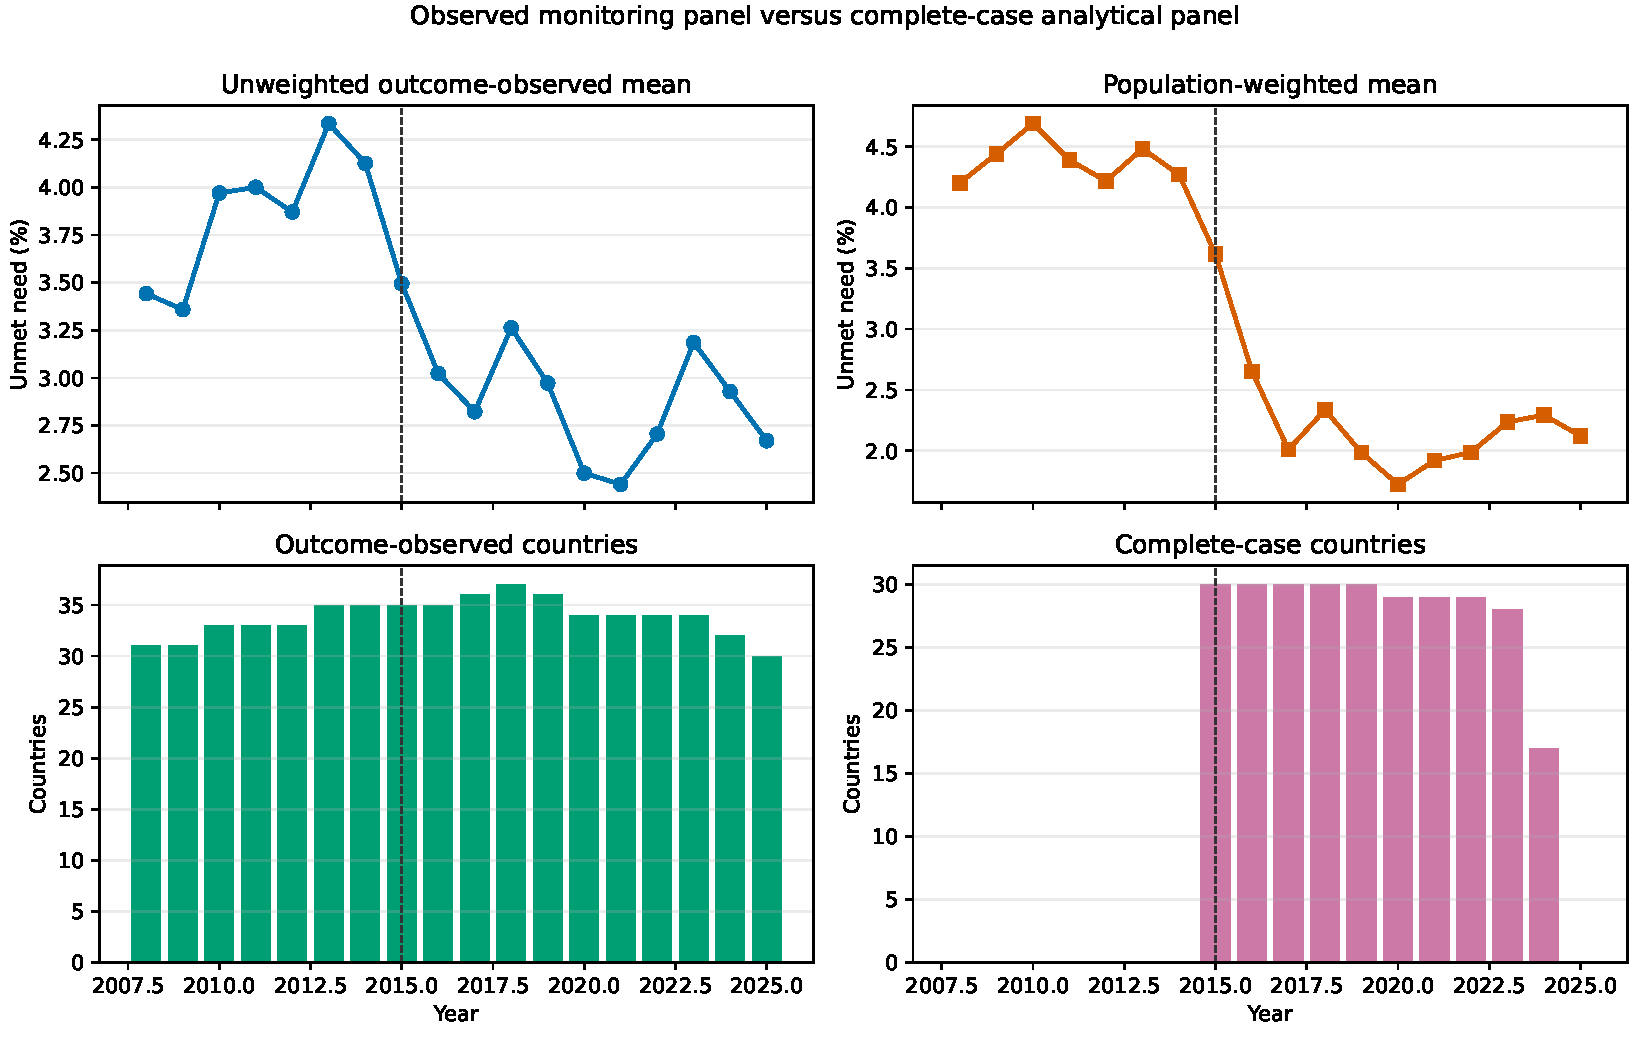
\includegraphics[width=0.96\textwidth]{descriptive_estimand_drift_diagnostic}
\caption{Observed monitoring panel versus complete-case analytical panel. The sample is observed \texttt{hlth\_silc\_08} country-years over 2008--2025; the population-weighted panel uses \texttt{demo\_pjan} country-year population normalized within year; complete-case counts use the baseline FE covariate-complete row set. Country coverage varies by year.}
\label{fig:descriptive_estimand_drift_diagnostic}
\end{figure}

The figure shows why a single monitoring average or a single regression coefficient is not self-explanatory. The unweighted and population-weighted series answer different monitoring questions: the former treats countries equally, while the latter gives larger within-year weight to countries with larger resident populations. The complete-case country count is a narrower object because it depends on covariate availability. This is the descriptive version of the estimand-drift problem analysed formally in Chapter~\ref{ch:modeling_strategy_results}.

The 2015 marker is a measurement-period warning, not a regression-discontinuity design. The outcome series covers years before and after 2015, but the baseline complete-case regression has too little pre-2015 covariate coverage to support a valid pre/post split for the poverty coefficient. Chapter~\ref{ch:modeling_strategy_results} therefore uses excluding-2015 and 2016-onward checks rather than treating the complete-case regression as a clean measurement-break design.

\section{Attrition Waterfall}

Figure~\ref{fig:complete_case_attrition_waterfall} and Table~\ref{tab:complete_case_attrition_waterfall} show the sequential row loss from the monitoring target to the baseline complete-case FE sample. The waterfall starts with all 608 outcome-observed country-years. It then requires GDP, unemployment, poverty or social exclusion, government health expenditure, and compulsory financing. The final step is the 282-row complete-case panel used for the baseline association model.

\begin{figure}[htbp]
\centering
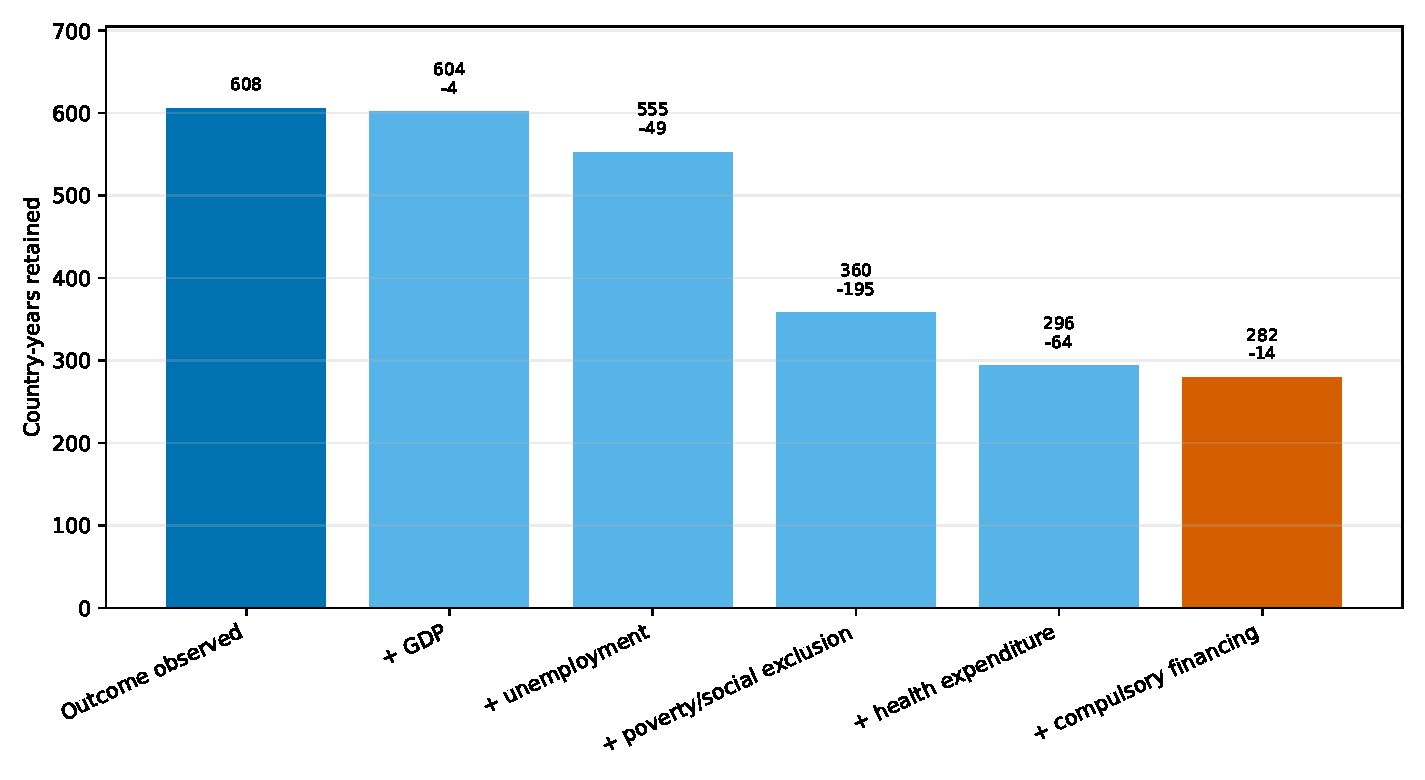
\includegraphics[width=0.92\textwidth]{complete_case_attrition_waterfall}
\caption{Complete-case attrition waterfall. The sample starts from all outcome-observed \texttt{hlth\_silc\_08} country-years over 2008--2025 and sequentially requires the baseline FE covariates; no population weights are applied and country coverage varies by year.}
\label{fig:complete_case_attrition_waterfall}
\end{figure}

\begin{table}[htbp]
\centering
\small
\caption{Sequential attrition from the outcome-observed monitoring panel to the baseline complete-case FE sample.}
\label{tab:complete_case_attrition_waterfall}
\begin{tabular}{@{}lrrrrr@{}}
\toprule
Step & Rows & Countries & Years & Rows lost & Retained pct \\
\midrule
Outcome observed & 608 & 37 & 18 & 0 & 100.0 \\
+ GDP & 604 & 36 & 18 & 4 & 99.3 \\
+ unemployment & 555 & 34 & 18 & 49 & 91.3 \\
+ poverty/social exclusion & 360 & 34 & 11 & 195 & 59.2 \\
+ health expenditure & 296 & 30 & 11 & 64 & 48.7 \\
+ compulsory financing & 282 & 30 & 10 & 14 & 46.4 \\
\bottomrule
\end{tabular}
\end{table}


The waterfall is the central descriptive result of the thesis. It shows that the baseline FE coefficient is not estimated on the full monitoring panel. It is estimated on a selected covariate-complete subset. The interpretation of the poverty/social-exclusion coefficient therefore depends not only on the regression formula, but also on the row-selection process that defines the analytical population.

\section{Where Attrition Occurs}

Table~\ref{tab:attrition_by_country_group} summarizes attrition by broad country group. Table~\ref{tab:attrition_by_covariate_block} shows how many outcome-observed rows remain when requiring each covariate block. These tables separate two mechanisms that would otherwise be hidden: country-group coverage differences and block-specific source availability.

\begin{table}[htbp]
\centering
\small
\caption{Attrition from outcome-observed rows to complete-case FE rows by country group.}
\label{tab:attrition_by_country_group}
\begin{tabular}{@{}lrrrrr@{}}
\toprule
Group & Outcome rows & CC rows & Countries & Rows lost & Retained pct \\
\midrule
East/South & 369 & 160 & 23 & 209 & 43.4 \\
West/North & 239 & 122 & 14 & 117 & 51.0 \\
\bottomrule
\end{tabular}
\end{table}


\begin{table}[H]
\centering
\small
\caption{Outcome-observed rows retained when requiring complete coverage by covariate block.}
\label{tab:attrition_by_covariate_block}
\begin{tabular}{@{}lrrrr@{}}
\toprule
Block & Rows & Countries & Years & Retained pct \\
\midrule
Outcome & 608 & 37 & 18 & 100.0 \\
Macroeconomic & 555 & 34 & 18 & 91.3 \\
Social vulnerability & 375 & 36 & 11 & 61.7 \\
Financing & 433 & 30 & 17 & 71.2 \\
Capacity & 426 & 29 & 16 & 70.1 \\
Inequality/labour & 392 & 34 & 12 & 64.5 \\
Population weights & 607 & 37 & 18 & 99.8 \\
\bottomrule
\end{tabular}

\vspace{0.2em}
\begin{minipage}{0.92\textwidth}\scriptsize \textit{Source:} Author's calculations from the merged Eurostat panel. Each row applies one covariate-block completeness requirement to the outcome-observed target; blocks are not cumulative.\end{minipage}
\end{table}


The block table is especially important because it distinguishes conceptual model breadth from empirical coverage. Adding covariates can make the model look more theoretically complete while moving the analysis further away from the outcome-observed monitoring target. The thesis therefore treats model expansion as an estimand choice, not merely as a technical adjustment.

Table~\ref{tab:leave_one_variable_out_sample_recovery} reports the sample recovery from omitting each baseline covariate from the complete-case requirement. It is not used to choose a preferred model mechanically. Its purpose is to show which variables contribute most to the difference between the broad monitoring target and the selected analytical panel.

\begin{table}[H]
\centering
\small
\caption{Sample recovery when each baseline covariate is omitted from the complete-case requirement.}
\label{tab:leave_one_variable_out_sample_recovery}
\begin{tabular}{@{}lrrrr@{}}
\toprule
Omitted covariate & Rows & Countries & Years & Rows recovered \\
\midrule
Poverty/social exclusion & 422 & 30 & 17 & 140 \\
Compulsory financing & 296 & 30 & 11 & 14 \\
Gov. health expenditure & 285 & 31 & 10 & 3 \\
Log GDP/capita & 282 & 30 & 10 & 0 \\
Unemployment & 282 & 30 & 10 & 0 \\
\bottomrule
\end{tabular}

\vspace{0.2em}
\begin{minipage}{0.92\textwidth}\scriptsize \textit{Source:} Author's calculations from the baseline covariate set. Rows recovered are measured relative to the 282-row complete-case sample.\end{minipage}
\end{table}


The country-level version is kept compact in the main text. Table~\ref{tab:attrition_by_country_top_loss} lists the countries with the lowest retention from outcome-observed rows to complete-case FE rows; the full country table is generated in the output folder and documented in the reproducibility appendix.

\begin{table}[H]
\centering
\small
\caption{Countries with the lowest retention from the outcome-observed target to the complete-case FE sample.}
\label{tab:attrition_by_country_top_loss}
\begin{tabular}{@{}lrrrr@{}}
\toprule
Country & Outcome rows & CC rows & Rows lost & Retained pct \\
\midrule
AL & 7 & 0 & 7 & 0.0 \\
ME & 11 & 0 & 11 & 0.0 \\
MK & 15 & 0 & 15 & 0.0 \\
RS & 13 & 0 & 13 & 0.0 \\
TR & 18 & 0 & 18 & 0.0 \\
UK & 11 & 0 & 11 & 0.0 \\
XK & 2 & 0 & 2 & 0.0 \\
NO & 18 & 8 & 10 & 44.4 \\
IS & 13 & 6 & 7 & 46.2 \\
BE & 18 & 9 & 9 & 50.0 \\
BG & 18 & 9 & 9 & 50.0 \\
CY & 18 & 9 & 9 & 50.0 \\
EL & 18 & 9 & 9 & 50.0 \\
ES & 18 & 9 & 9 & 50.0 \\
\bottomrule
\end{tabular}

\vspace{0.2em}
\begin{minipage}{0.92\textwidth}\scriptsize \textit{Source:} Author's calculations from the merged Eurostat panel. The table reports the lowest country-level retention rates without assigning substantive regional labels.\end{minipage}
\end{table}


\section{Included and Excluded Rows}

The most important question is whether excluded rows look like a neutral remainder. They do not. Table~\ref{tab:included_vs_excluded_smd} reports standardized mean differences between complete-case rows and excluded outcome-observed rows. Table~\ref{tab:missingness_comparison} reports the corresponding descriptive mean comparison.

\begin{table}[H]
\centering
\small
\caption{Standardized mean differences between complete-case rows and excluded outcome-observed rows.}
\label{tab:included_vs_excluded_smd}
\begin{tabular}{@{}lrrrrr@{}}
\toprule
Variable & Included N & Included mean & Excluded N & Excluded mean & SMD \\
\midrule
Unmet need & 282 & 2.63 & 326 & 3.85 & -0.37 \\
GDP/capita & 282 & 36851.38 & 322 & 26235.31 & 0.46 \\
Unemployment & 282 & 6.86 & 274 & 10.48 & -0.76 \\
Poverty/social exclusion & 282 & 21.00 & 93 & 28.39 & -0.90 \\
Gov. health expenditure & 282 & 6.37 & 220 & 6.17 & 0.13 \\
Compulsory financing & 282 & 6.54 & 162 & 6.50 & 0.03 \\
\bottomrule
\end{tabular}

\vspace{0.2em}
\begin{minipage}{0.92\textwidth}\scriptsize \textit{Source:} Author's calculations from the 608 outcome-observed \texttt{hlth\_silc\_08} rows. SMDs compare the 282 complete cases with rows excluded by missing baseline covariates.\end{minipage}
\end{table}


\begin{table}[htbp]
\centering
\caption{Included versus excluded outcome-observed rows}
\label{tab:missingness_comparison}
\begingroup
\small
\begin{tabular}{@{}lrrrrrr@{}}
\toprule
Variable & Inc. \(N\) & Inc. mean & Exc. \(N\) & Exc. mean & Diff. & p-value \\
\midrule
Unmet need & 282 & 2.63 & 326 & 3.85 & -1.23 & <0.001 \\
GDP/cap. & 282 & 36851.38 & 322 & 26235.31 & 10616.07 & <0.001 \\
Unemp. & 282 & 6.86 & 274 & 10.48 & -3.62 & <0.001 \\
Poverty & 282 & 21.00 & 93 & 28.39 & -7.39 & <0.001 \\
\bottomrule
\end{tabular}

\vspace{0.2em}
\begin{minipage}{0.92\textwidth}\scriptsize Notes: Welch tests compare rows included in the baseline complete-case regression with outcome-observed rows excluded because at least one baseline covariate is missing. The table is descriptive and is used as a selection diagnostic.\end{minipage}
\endgroup

\end{table}

These diagnostics are not interpreted as a correction. They show why correction is needed conceptually and why any single complete-case coefficient must be read as a selected-panel estimate. If excluded rows have different unmet need and macro-social conditions, the complete-case panel is not simply a smaller version of the monitoring panel.

\section{Coverage Heatmaps}

Figure~\ref{fig:missingness_heatmap_socioeconomic} and Figure~\ref{fig:missingness_heatmap_financing} split the missingness heatmaps into readable covariate blocks. The heatmaps show country-year coverage, not model results. Their value is diagnostic: they make visible that Eurostat covariate availability has structure by country, period, and indicator block.

\begin{figure}[htbp]
\centering
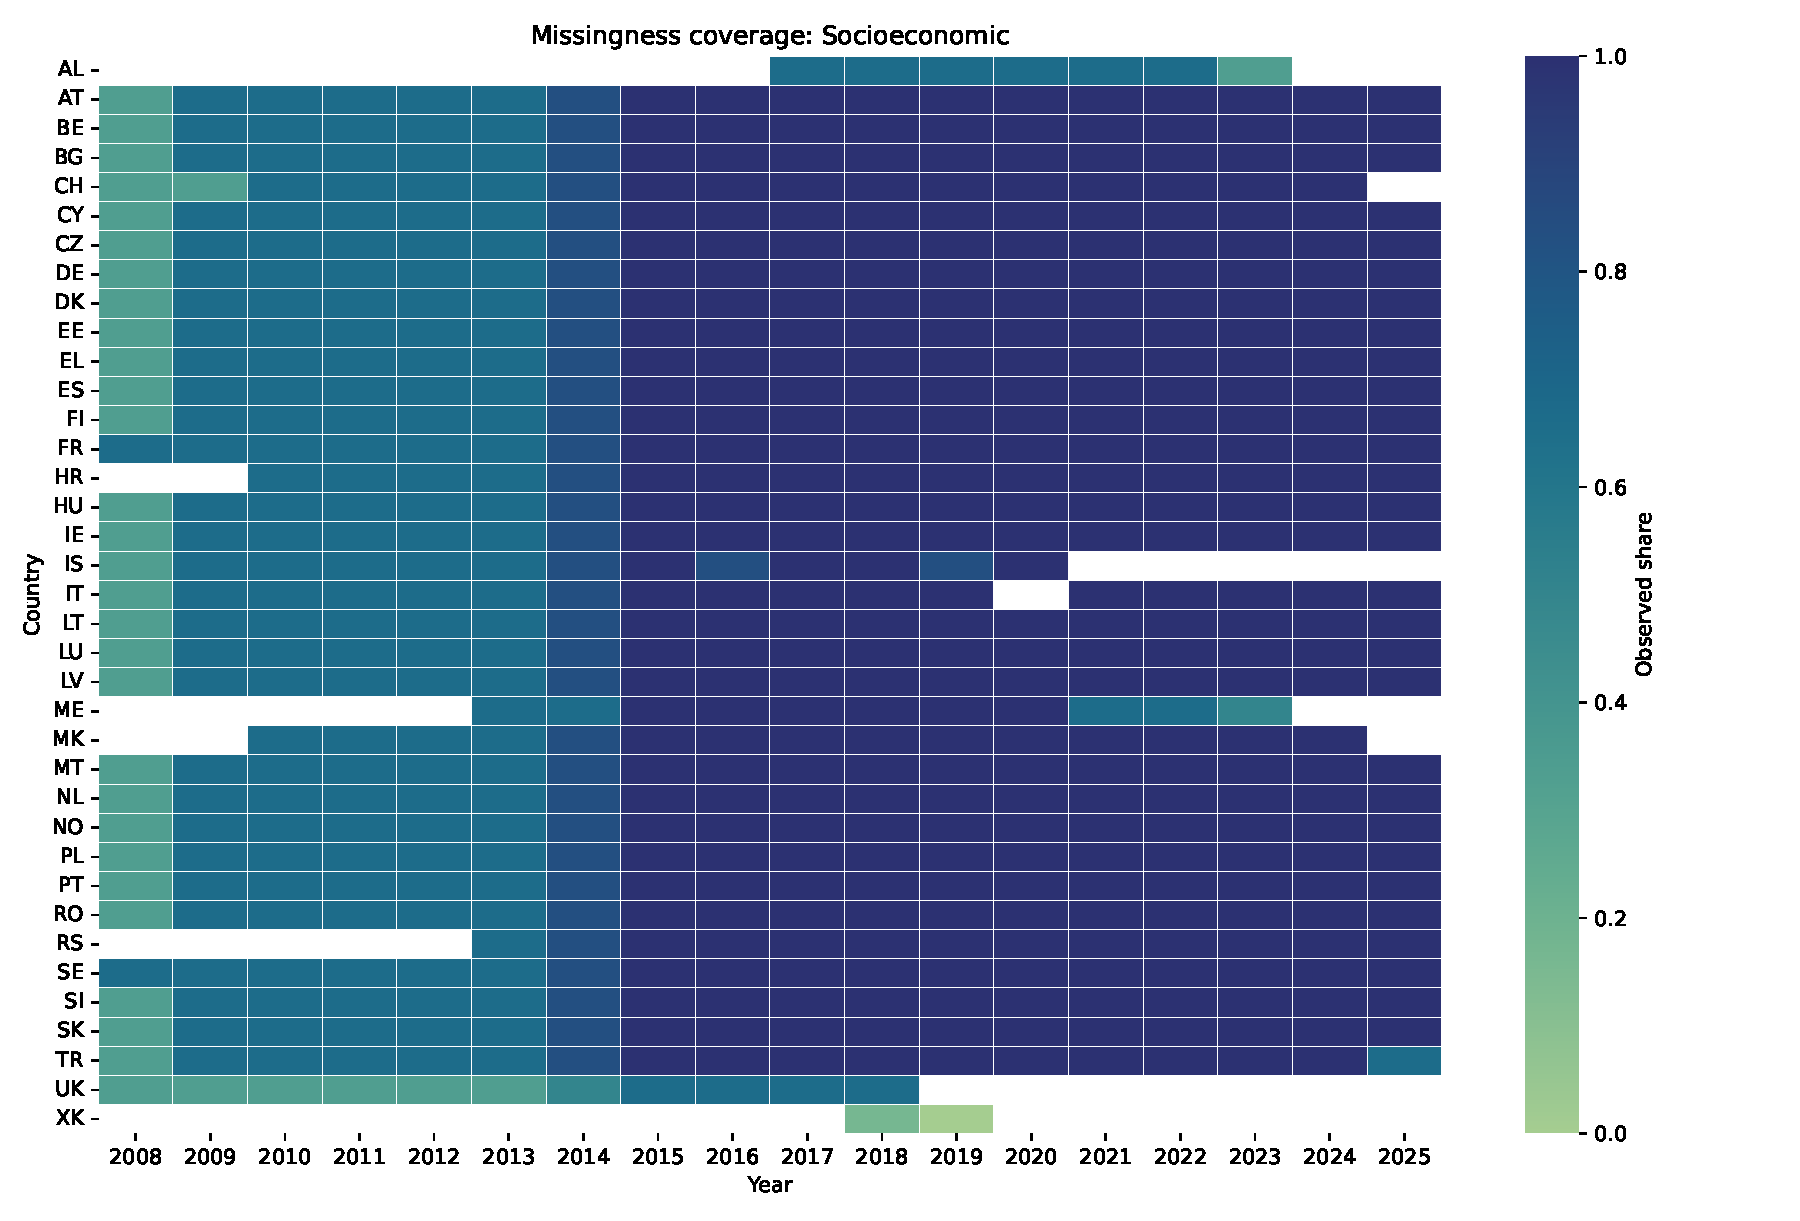
\includegraphics[width=0.96\textwidth]{missingness_heatmap_socioeconomic}
\caption{Socioeconomic covariate coverage. Cells show the observed share among socioeconomic variables in each country-year over 2008--2025; no population weights are applied and blank or low-coverage cells indicate missing source coverage.}
\label{fig:missingness_heatmap_socioeconomic}
\end{figure}

\begin{figure}[htbp]
\centering
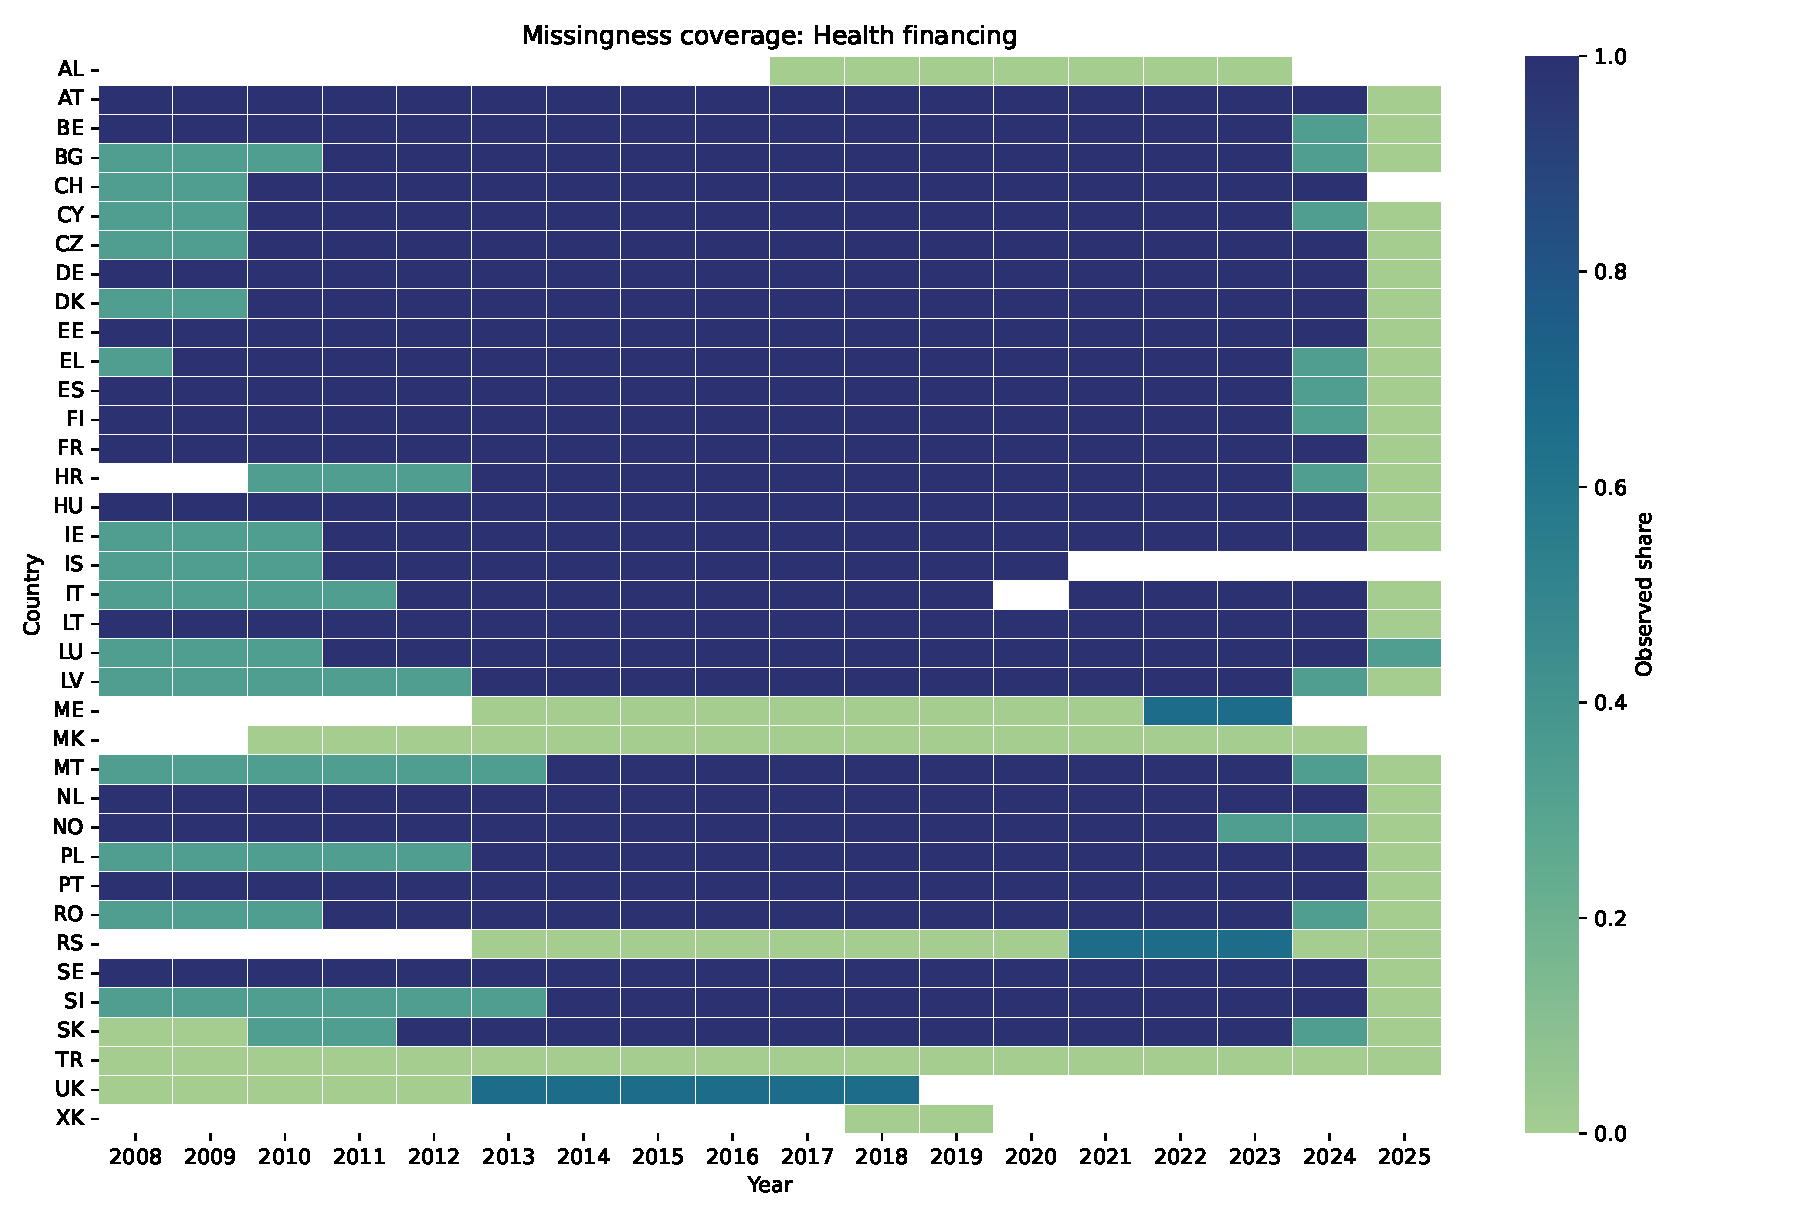
\includegraphics[width=0.96\textwidth]{missingness_heatmap_financing}
\caption{Health-financing covariate coverage. Cells show the observed share among financing variables in each country-year over 2008--2025; no population weights are applied and country coverage varies by indicator and year.}
\label{fig:missingness_heatmap_financing}
\end{figure}

\section{Country Heterogeneity as Context}

Country heterogeneity remains useful, but it is no longer the centre of the chapter. Figure~\ref{fig:descriptive_country_rankings} ranks countries by the latest observed value of unmet medical care need. Figure~\ref{fig:descriptive_country_year_heatmap} shows the same outcome in country-year form. These figures motivate country structure in the models and help interpret why a selected complete-case panel may not represent the same monitoring object as the full outcome-observed panel.

\begin{figure}[htbp]
\centering
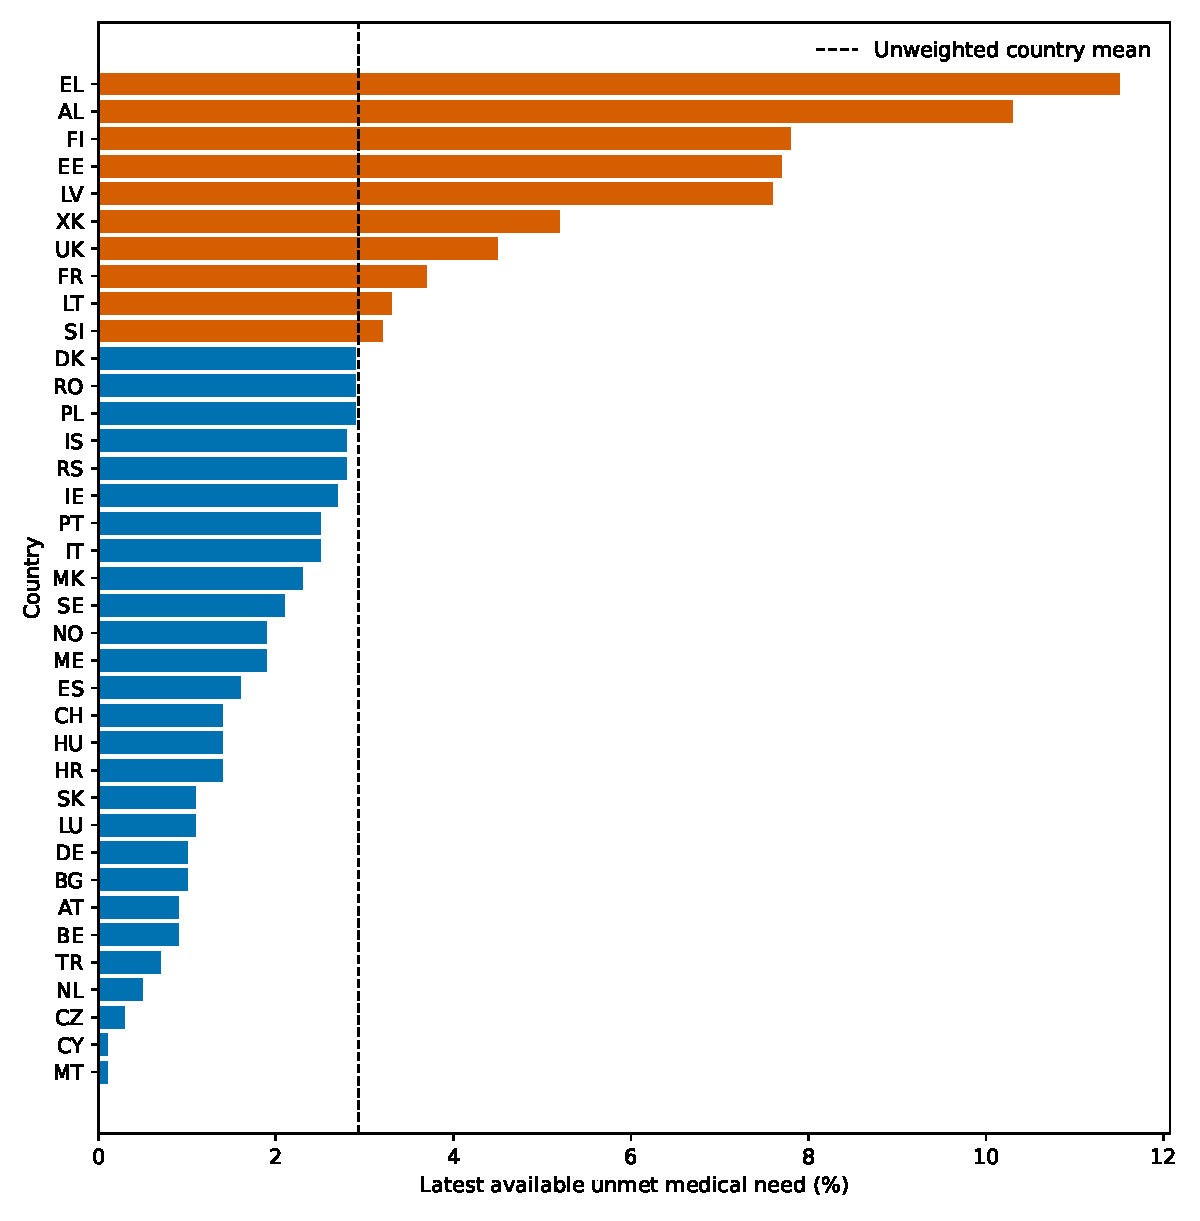
\includegraphics[width=0.88\textwidth]{descriptive_country_rankings}
\caption{Country rankings in unmet medical care need. Rankings use the latest observed \texttt{hlth\_silc\_08} value per country in the 2008--2025 descriptive panel; no population weights are applied and the latest year can differ where country coverage varies.}
\label{fig:descriptive_country_rankings}
\end{figure}

\begin{figure}[htbp]
\centering
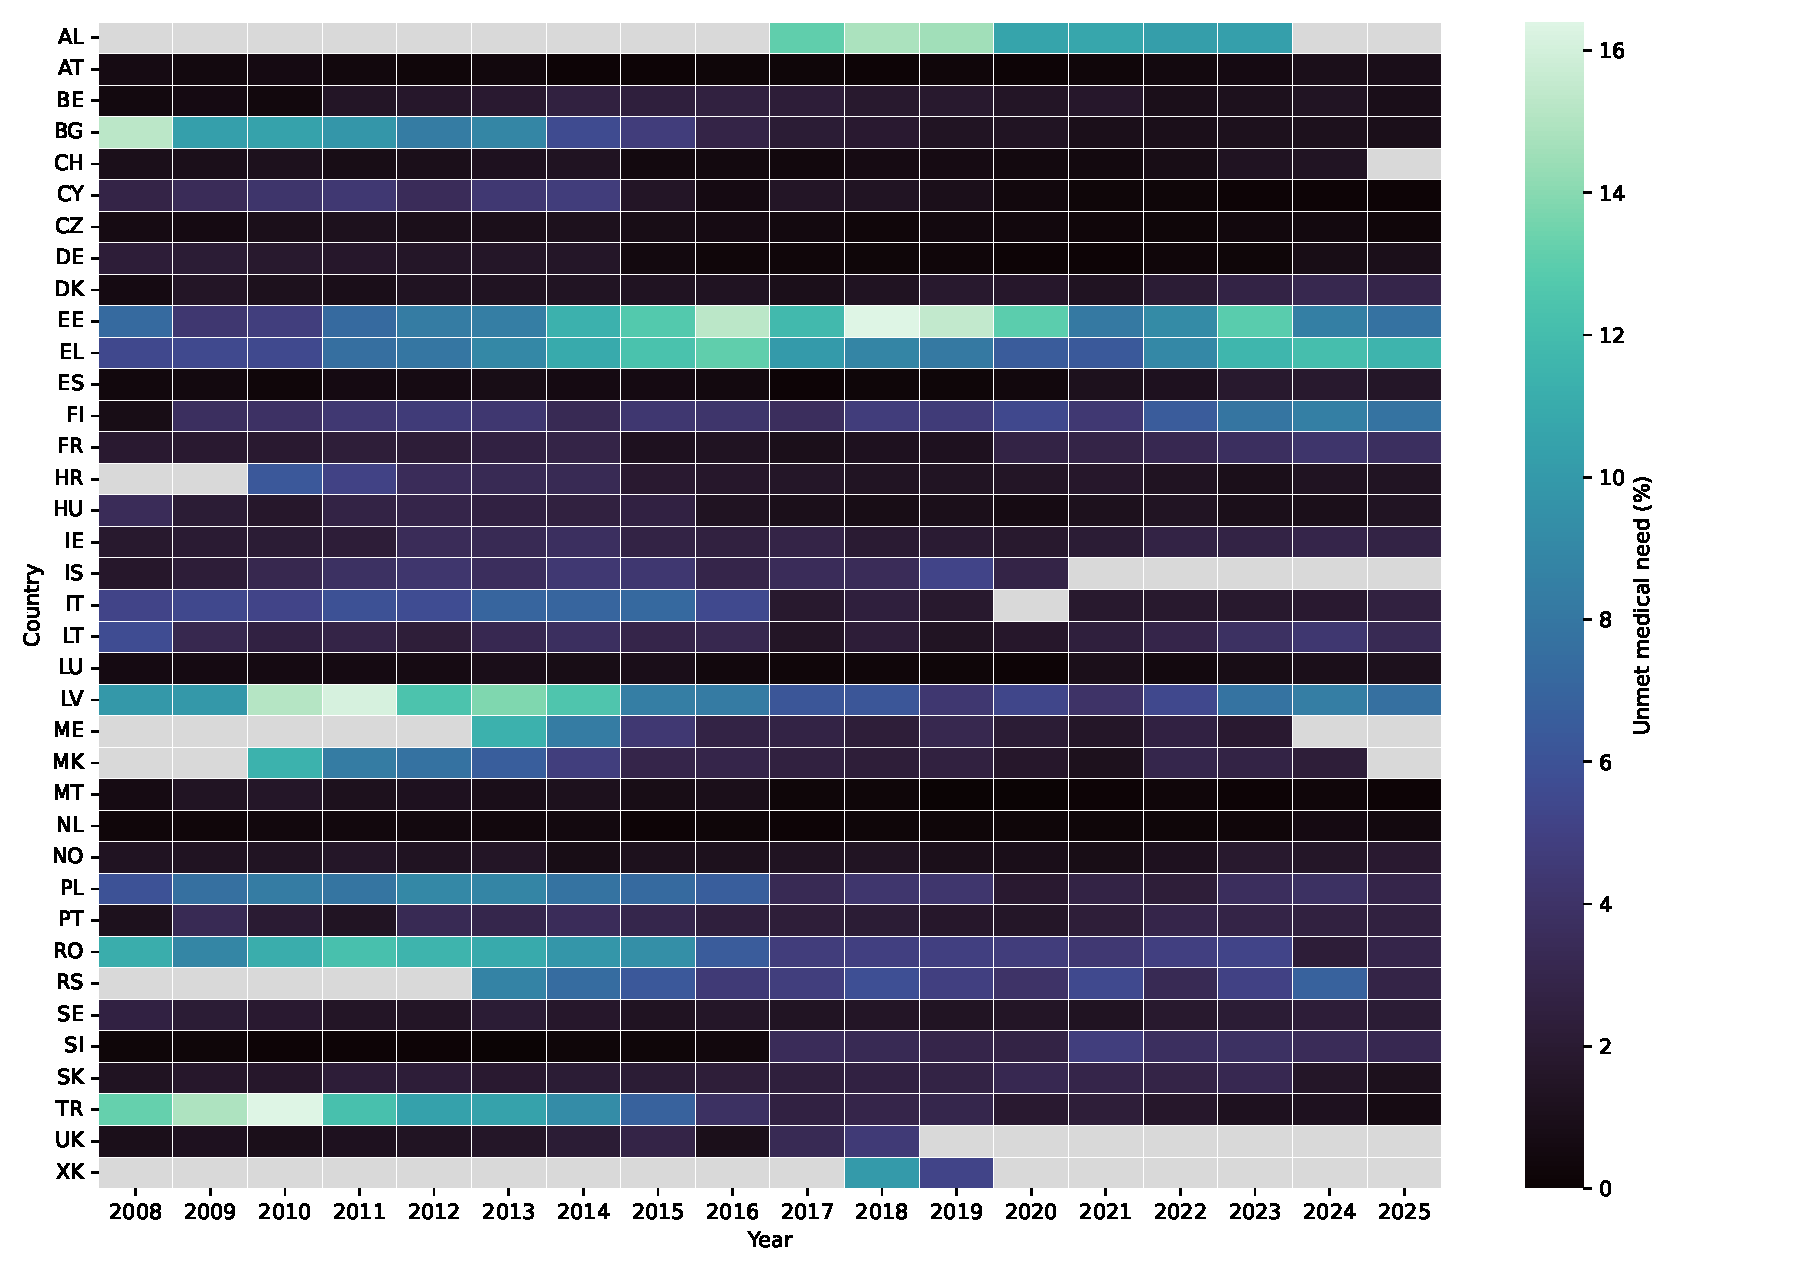
\includegraphics[width=0.96\textwidth]{descriptive_country_year_heatmap}
\caption{Country-year heatmap of unmet medical care need. Cells show observed \texttt{hlth\_silc\_08} values over 2008--2025; blank cells indicate missing country-year outcome coverage; no population weights are applied.}
\label{fig:descriptive_country_year_heatmap}
\end{figure}

\section{Secondary Descriptive Outputs}

Several descriptive outputs are generated for reproducibility but do not carry the thesis argument. Bivariate scatterplots are screening diagnostics only because they do not condition on country or year structure. Convergence outputs are interpreted as descriptive context and remain vulnerable to regression-to-the-mean and changing coverage. Citizenship gaps are descriptive equity context because aggregate citizenship rows cannot adjust for income, health status, legal status, language, duration of residence, or local access conditions. The \texttt{hlth\_silc\_08b} comparison is a denominator robustness check for 2021--2025 only. These materials support transparency, but they do not compete with the target-population drift analysis.

\chapter{Target-Population Sensitivity and Regression Results}
\label{ch:modeling_strategy_results}

\section{Empirical Estimand Ladder}

This chapter is the empirical core of the thesis. It applies the framework defined in Chapter~\ref{ch:framework} to the Eurostat unmet-care panels. The poverty or social-exclusion coefficient is treated as a stress-test coefficient: it is followed as the model moves from the intended outcome-observed monitoring panel to selected complete cases, population-weighted complete cases, universe-restricted panels, IPW diagnostics, MAR imputation, and MNAR stress tests. The question is not whether one selected-panel coefficient is statistically marked. The question is whether the aggregate poverty association is stable when the target population, weighting rule, row-selection process, and missing-data assumption change.

\begin{table}[htbp]
\centering
\scriptsize
\caption{Target populations, assumptions, and interpretation of estimates. Row counts come from the generated thesis pipeline and distinguish the 608-row outcome-observed target from the 282-row complete-case FE sample.}
\label{tab:estimand_framework}
\resizebox{\textwidth}{!}{%
\begin{tabular}{@{}p{0.16\textwidth}p{0.25\textwidth}rrp{0.20\textwidth}p{0.25\textwidth}@{}}
\toprule
Label & Target population & Countries & Rows & Weighting & Interpretation \\
\midrule
Outcome-observed & All country-years with observed \texttt{hlth\_silc\_08} & 37 & 608 & None & Average-country monitoring target before covariate attrition. \\
Population-weighted & Outcome-observed or selected rows with valid \texttt{demo\_pjan} & 37 & 607 & Year-normalized population & Average-resident monitoring target; not inherently more correct. \\
Complete-case FE & Outcome and all baseline regression covariates observed & 30 & 282 & None & Selected analytical panel for the baseline FE coefficient. \\
Balanced-outcome & Countries with complete primary-outcome and population-weight coverage & 25 & 238 & Optional & Coverage-restricted target; not automatically covariate-balanced. \\
IPW CC & Complete cases reweighted by predicted complete-case inclusion & 30 & 282 & Stabilized truncated IPW & Selection diagnostic; cannot recover structurally missing covariates. \\
MAR MI & Outcome-observed rows with model-imputed covariates & 37 & 608 & Usually none & Model-based sensitivity target under imputation assumptions. \\
MNAR sensitivity & Outcome-observed rows with shifted imputed values & 37 & 608 & Scenario-specific & Stress test for departures from MAR; implemented in Step 2. \\
\bottomrule
\end{tabular}%
}

\vspace{0.2em}
\begin{minipage}{0.96\textwidth}\scriptsize Notes: Row counts refer to the generated thesis pipeline. Balanced-outcome means balanced for the primary outcome and population weights, not for every regression covariate. MAR and MNAR imputation estimates are model-based sensitivity estimates.\end{minipage}

\vspace{0.25em}

\begin{minipage}{0.96\textwidth}
\scriptsize \textit{Source:} Author's synthesis from the thesis data pipeline and missing-data literature \citep{little_rubin_2019,seaman_white_2013}. The table is a conceptual map for interpreting generated estimates, not an external empirical result.
\end{minipage}
\end{table}

The hierarchy is estimand-first. Complete-case and population-weighted complete-case estimates use the same selected rows but answer different country-versus-resident monitoring questions. Balanced-outcome means balanced for the primary outcome and valid population weights, not covariate-balanced. IPW is a selection diagnostic among observed complete cases. MAR and MNAR MI rows target the broader outcome-observed panel under explicit model-based assumptions and are not treated as corrected estimates \citep{rubin_1987,little_rubin_2019}.

\section{Multi-Outcome Target-Population Drift Diagnostics}

Before estimating poverty/social-exclusion coefficients, the audit protocol asks how far each feasible outcome can travel from the monitoring target to an analytical sample. Table~\ref{tab:multi_outcome_attrition_matrix} reports this drift across the multi-outcome registry. The columns are sequential requirements: outcome observed, valid population weight, GDP, unemployment, poverty/social exclusion, the baseline financing-complete covariate set, and a stricter capacity-augmented sensitivity set.

The matrix shows that target-population drift is not a one-off feature of the primary medical indicator. Long population-denominator medical and dental indicators have broad monitoring coverage, but their baseline complete-case analytical samples are much smaller. Need-denominator indicators are shorter by construction and become especially limited once financing and capacity covariates are required. These rows do not estimate any substantive effect; they define which empirical targets are supportable.

Figure~\ref{fig:multi_outcome_retention_heatmap} visualizes the same row-retention problem. The heatmap is useful because it separates denominator limits from covariate-completeness limits. A short need-denominator indicator may be feasible for monitoring but weak for regression once country-year covariates are required.

The detailed 608-to-282 primary-outcome sequence is reported once in Figure~\ref{fig:complete_case_attrition_waterfall} and Table~\ref{tab:complete_case_attrition_waterfall}. The multi-outcome matrix and retention heatmap extend that diagnostic across outcomes without repeating the primary waterfall.

Table~\ref{tab:multi_outcome_included_excluded_smd_top} shows that attrition is not only about row counts. Excluded rows differ from included rows on variables tied to vulnerability and system capacity. The direction and size of these differences vary by indicator length and denominator, which is why the later coefficient matrix labels infeasible or unstable estimands instead of forcing them into one preferred model.

\begin{table}[H]
\centering
\scriptsize
\caption{Multi-outcome attrition matrix. Rows are feasible Eurostat unmet-care indicators; columns report retained country-year rows after sequentially requiring population weights and covariate blocks. Baseline CC is the financing-complete fixed-effects covariate set used for the primary poverty stress test, while capacity is a stricter sensitivity requirement.}
\label{tab:multi_outcome_attrition_matrix}
\begin{tabular}{p{0.24\linewidth}rrrrrrr}
\toprule
Indicator & Outcome & Pop. & GDP & Unemp. & Poverty & Baseline CC & Capacity \\
\midrule
Dental need & 154 & 154 & 152 & 147 & 147 & 93 & 69 \\
Dental population & 607 & 606 & 604 & 555 & 360 & 282 & 233 \\
Medical need & 154 & 154 & 152 & 147 & 147 & 93 & 69 \\
Medical population & 608 & 607 & 604 & 555 & 360 & 282 & 233 \\
Medical cost & 608 & 607 & 604 & 555 & 360 & 282 & 233 \\
Medical distance & 608 & 607 & 604 & 555 & 360 & 282 & 233 \\
Medical waiting & 608 & 607 & 604 & 555 & 360 & 282 & 233 \\
\bottomrule
\end{tabular}

\vspace{0.25em}

\begin{minipage}{0.96\textwidth}
\scriptsize \textit{Source:} Author's calculations from the multi-outcome Eurostat panel and \texttt{demo\_pjan}. The table is a target-support diagnostic: it reports which outcome-by-covariate targets can support later estimands.
\end{minipage}
\end{table}

\begin{figure}[H]
\centering
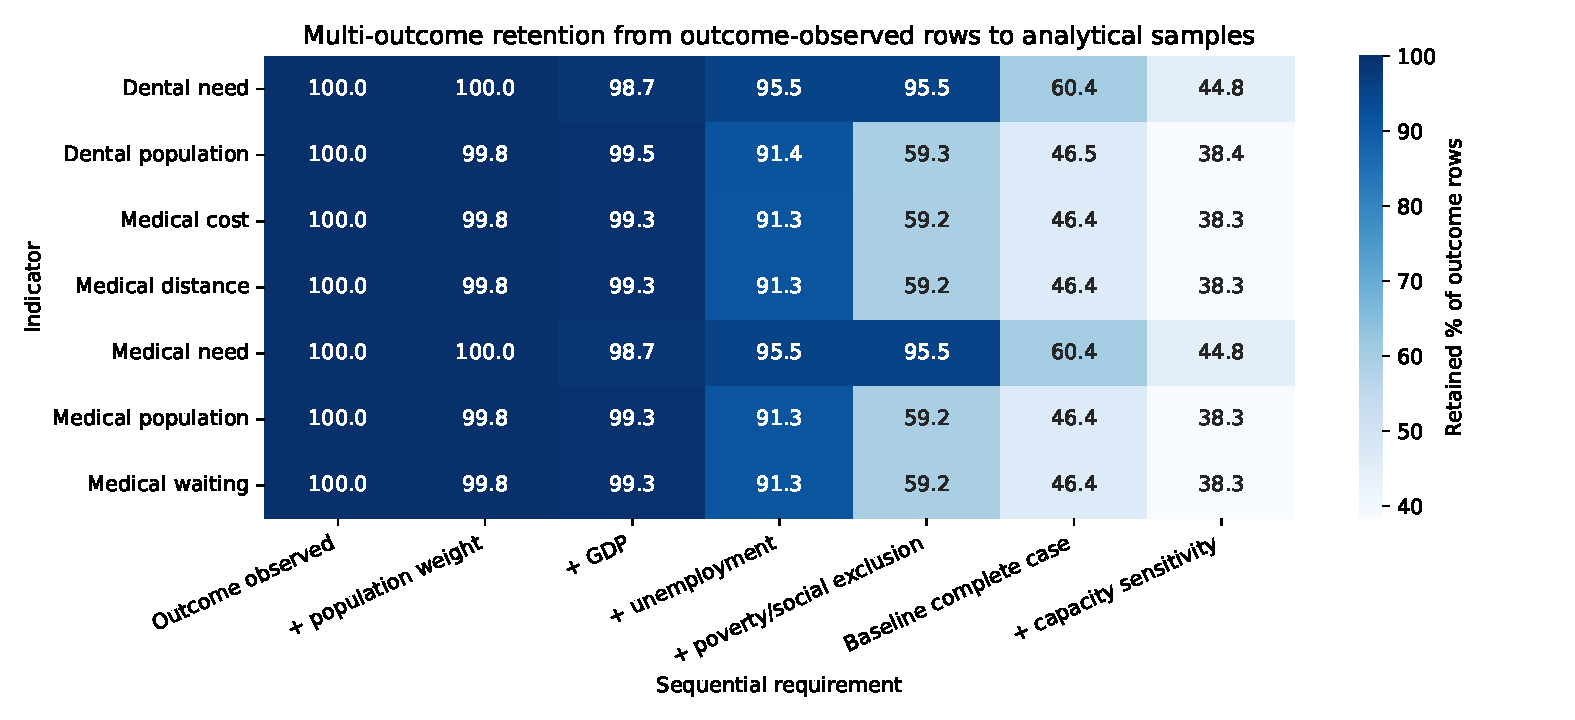
\includegraphics[width=0.95\textwidth]{multi_outcome_retention_heatmap}
\caption{Multi-outcome retention heatmap. Cells report the percentage of each indicator's outcome-observed country-years retained after sequential population-weight and covariate requirements; no regression is estimated in this diagnostic.}
\label{fig:multi_outcome_retention_heatmap}
\vspace{0.25em}

\begin{minipage}{0.94\textwidth}
\scriptsize \textit{Source:} Author's calculations from the multi-outcome Eurostat panel. Retention is measured relative to each indicator's own outcome-observed country-year target.
\end{minipage}
\end{figure}

\begin{table}[H]
\centering
\scriptsize
\caption{Largest included-versus-excluded standardized differences by outcome. Included rows are baseline complete-case rows for each outcome; excluded rows are outcome-observed rows removed by missing baseline covariates. SMDs are descriptive selection diagnostics.}
\label{tab:multi_outcome_included_excluded_smd_top}
\begin{tabular}{p{0.20\linewidth}p{0.21\linewidth}rrrrr}
\toprule
Indicator & Variable & In N & Excl. N & In mean & Excl. mean & SMD \\
\midrule
Dental need & physicians\_per\_100k & 71 & 7 & 413.741 & 326.734 & 1.187 \\
Dental need & poverty\_or\_social\_exclusion\_pc & 93 & 61 & 20.304 & 24.361 & -0.63 \\
Dental population & physicians\_per\_100k & 236 & 195 & 385.83 & 325.958 & 0.907 \\
Dental population & poverty\_or\_social\_exclusion\_pc & 282 & 93 & 21.0 & 28.39 & -0.903 \\
Medical need & physicians\_per\_100k & 71 & 7 & 413.741 & 326.734 & 1.187 \\
Medical need & poverty\_or\_social\_exclusion\_pc & 93 & 61 & 20.304 & 24.361 & -0.63 \\
Medical population & physicians\_per\_100k & 236 & 195 & 385.83 & 325.958 & 0.907 \\
Medical population & poverty\_or\_social\_exclusion\_pc & 282 & 93 & 21.0 & 28.39 & -0.903 \\
Medical cost & physicians\_per\_100k & 236 & 195 & 385.83 & 325.958 & 0.907 \\
Medical cost & poverty\_or\_social\_exclusion\_pc & 282 & 93 & 21.0 & 28.39 & -0.903 \\
Medical distance & physicians\_per\_100k & 236 & 195 & 385.83 & 325.958 & 0.907 \\
Medical distance & poverty\_or\_social\_exclusion\_pc & 282 & 93 & 21.0 & 28.39 & -0.903 \\
Medical waiting & physicians\_per\_100k & 236 & 195 & 385.83 & 325.958 & 0.907 \\
Medical waiting & poverty\_or\_social\_exclusion\_pc & 282 & 93 & 21.0 & 28.39 & -0.903 \\
\bottomrule
\end{tabular}

\vspace{0.25em}

\begin{minipage}{0.96\textwidth}
\scriptsize \textit{Source:} Author's calculations from feasible Eurostat unmet-care indicators and baseline covariates. SMDs diagnose selection distortion; they are not regression coefficients.
\end{minipage}
\end{table}

\FloatBarrier

\section{Outcome-by-Estimand Coefficient Matrix}

Table~\ref{tab:outcome_estimand_coefficient_matrix} replaces a long list of separate robustness rows with a single outcome-by-estimand audit. For each feasible outcome, the table follows the poverty/social-exclusion coefficient across five estimand families: unweighted complete-case FE, population-weighted complete-case FE, balanced-outcome FE, IPW complete-case FE, and MAR MI full-target FE. Rows that do not meet the minimum support rule are reported as infeasible rather than forced.

The matrix changes the interpretation of the empirical evidence. Long population-denominator indicators can support several observed-data estimands. Need-denominator indicators are useful for monitoring, but their observed complete-case FE rows are too short for the deterministic support rule and are therefore non-identifiable as complete-case regression targets. MAR MI can still be estimated for those shorter targets, but one imputed estimand family is not enough to support a stable coefficient interpretation.

Figure~\ref{fig:outcome_estimand_coefficient_stability} shows the core empirical contribution of the chapter. Observed complete-case estimands often remain positive, while MAR MI full-target estimates can move toward zero or change sign. The result is a coefficient-stability audit: the same poverty/social-exclusion stress-test variable has different interpretations under different target populations and missing-data assumptions.

Table~\ref{tab:drift_stability_summary} translates the coefficient matrix into the framework metrics defined in Chapter~\ref{ch:framework}. The poverty/social-exclusion coefficient remains a stress-test coefficient, not the thesis contribution. The standardized coefficient \(\theta\) puts coefficients on a comparable IQR scale across outcomes; \(\theta\) IQR summarizes dispersion across feasible estimand families; directional agreement records whether signs agree with the observed-data reference direction; and CSI applies the declared \(\delta=0.10\) tolerance rule. The final labels are deterministic diagnostic labels, not causal claims and not evidence of individual-level mechanisms.

\begin{table}[H]
\centering
\scriptsize
\caption{Outcome-by-estimand coefficient matrix for the poverty/social-exclusion coefficient. Each row defines a distinct target population and missing-data assumption; infeasible rows are retained with the reason. MAR MI is interpreted as model-based sensitivity, not as correction.}
\label{tab:outcome_estimand_coefficient_matrix}
\begingroup
\scriptsize
\setlength{\tabcolsep}{2pt}
\renewcommand{\arraystretch}{0.92}
\begin{longtable}{@{}p{0.13\linewidth}p{0.16\linewidth}rrrp{0.055\linewidth}p{0.135\linewidth}p{0.055\linewidth}p{0.15\linewidth}@{}}
\caption{Outcome-by-estimand coefficient matrix for the poverty/social-exclusion coefficient. Each row defines a distinct target population and missing-data assumption; infeasible rows are retained with the reason. MAR MI is interpreted as model-based sensitivity, not as correction.}\label{tab:outcome_estimand_coefficient_matrix}\\
\toprule
Indicator & Estimand & Rows & Ctries & Years & Coef. & 95\% CI & p & Status \\
\midrule
\endfirsthead
\caption[]{Outcome-by-estimand coefficient matrix for the poverty/social-exclusion coefficient. Each row defines a distinct target population and missing-data assumption; infeasible rows are retained with the reason. MAR MI is interpreted as model-based sensitivity, not as correction. (continued)}\\
\toprule
Indicator & Estimand & Rows & Ctries & Years & Coef. & 95\% CI & p & Status \\
\midrule
\endhead
\midrule
\multicolumn{9}{r}{\scriptsize Continued on next page}\\
\endfoot
\bottomrule
\endlastfoot
Dental need & Unweighted CC FE & 93 & 28 & 4 &  &  &  & infeas.: rows<100 \\
Dental need & Pop.-weighted CC FE & 93 & 28 & 4 &  &  &  & infeas.: rows<100 \\
Dental need & Balanced FE & 86 & 24 & 4 &  &  &  & infeas.: rows<100 \\
Dental need & IPW CC FE & 93 & 28 & 4 &  &  &  & infeas.: rows<100 \\
Dental need & MAR MI full target & 154 & 34 & 5 & -0.232 & [-0.929, 0.465] & 0.514 & est. \\
Dental population & Unweighted CC FE & 282 & 30 & 10 & 0.203 & [-0.066, 0.471] & 0.139 & est. \\
Dental population & Pop.-weighted CC FE & 282 & 30 & 10 & 0.491 & [0.029, 0.953] & 0.037 & est. \\
Dental population & Balanced FE & 238 & 25 & 10 & 0.226 & [0.068, 0.383] & 0.005 & est. \\
Dental population & IPW CC FE & 282 & 30 & 10 & 0.220 & [-0.103, 0.544] & 0.182 & est. \\
Dental population & MAR MI full target & 607 & 37 & 18 & -0.009 & [-0.096, 0.079] & 0.848 & est. \\
Medical need & Unweighted CC FE & 93 & 28 & 4 &  &  &  & infeas.: rows<100 \\
Medical need & Pop.-weighted CC FE & 93 & 28 & 4 &  &  &  & infeas.: rows<100 \\
Medical need & Balanced FE & 86 & 24 & 4 &  &  &  & infeas.: rows<100 \\
Medical need & IPW CC FE & 93 & 28 & 4 &  &  &  & infeas.: rows<100 \\
Medical need & MAR MI full target & 154 & 34 & 5 & 0.094 & [-0.132, 0.320] & 0.414 & est. \\
Medical population & Unweighted CC FE & 282 & 30 & 10 & 0.178 & [0.046, 0.309] & 0.008 & est. \\
Medical population & Pop.-weighted CC FE & 282 & 30 & 10 & 0.304 & [-0.007, 0.615] & 0.055 & est. \\
Medical population & Balanced FE & 238 & 25 & 10 & 0.154 & [0.060, 0.248] & 0.001 & est. \\
Medical population & IPW CC FE & 282 & 30 & 10 & 0.214 & [0.060, 0.367] & 0.006 & est. \\
Medical population & MAR MI full target & 608 & 37 & 18 & -0.012 & [-0.098, 0.074] & 0.789 & est. \\
Medical cost & Unweighted CC FE & 282 & 30 & 10 & 0.183 & [0.088, 0.277] & <.001 & est. \\
Medical cost & Pop.-weighted CC FE & 282 & 30 & 10 & 0.299 & [0.066, 0.533] & 0.012 & est. \\
Medical cost & Balanced FE & 238 & 25 & 10 & 0.146 & [0.083, 0.208] & <.001 & est. \\
Medical cost & IPW CC FE & 282 & 30 & 10 & 0.230 & [0.099, 0.362] & <.001 & est. \\
Medical cost & MAR MI full target & 608 & 37 & 18 & 0.019 & [-0.061, 0.100] & 0.640 & est. \\
Medical distance & Unweighted CC FE & 282 & 30 & 10 & 0.008 & [-0.002, 0.018] & 0.097 & est. \\
Medical distance & Pop.-weighted CC FE & 282 & 30 & 10 & 0.018 & [0.000, 0.036] & 0.048 & est. \\
Medical distance & Balanced FE & 238 & 25 & 10 & 0.011 & [0.003, 0.020] & 0.007 & est. \\
Medical distance & IPW CC FE & 282 & 30 & 10 & 0.007 & [-0.002, 0.016] & 0.148 & est. \\
Medical distance & MAR MI full target & 608 & 37 & 18 & 0.002 & [-0.004, 0.007] & 0.524 & est. \\
Medical waiting & Unweighted CC FE & 282 & 30 & 10 & -0.010 & [-0.055, 0.035] & 0.671 & est. \\
Medical waiting & Pop.-weighted CC FE & 282 & 30 & 10 & -0.004 & [-0.079, 0.072] & 0.927 & est. \\
Medical waiting & Balanced FE & 238 & 25 & 10 & -0.001 & [-0.045, 0.043] & 0.973 & est. \\
Medical waiting & IPW CC FE & 282 & 30 & 10 & -0.009 & [-0.056, 0.038] & 0.704 & est. \\
Medical waiting & MAR MI full target & 608 & 37 & 18 & -0.001 & [-0.041, 0.039] & 0.966 & est. \\
\end{longtable}
\endgroup

\vspace{0.25em}

\begin{minipage}{0.96\textwidth}
\scriptsize \textit{Source:} Author's estimates from the thesis regression and imputation pipeline. Observed-data cells use country-and-year FE where feasible; MAR MI cells pool imputed outcome-observed panels using Rubin's rules \citep{rubin_1987,little_rubin_2019}.
\end{minipage}
\end{table}

\begin{figure}[H]
\centering
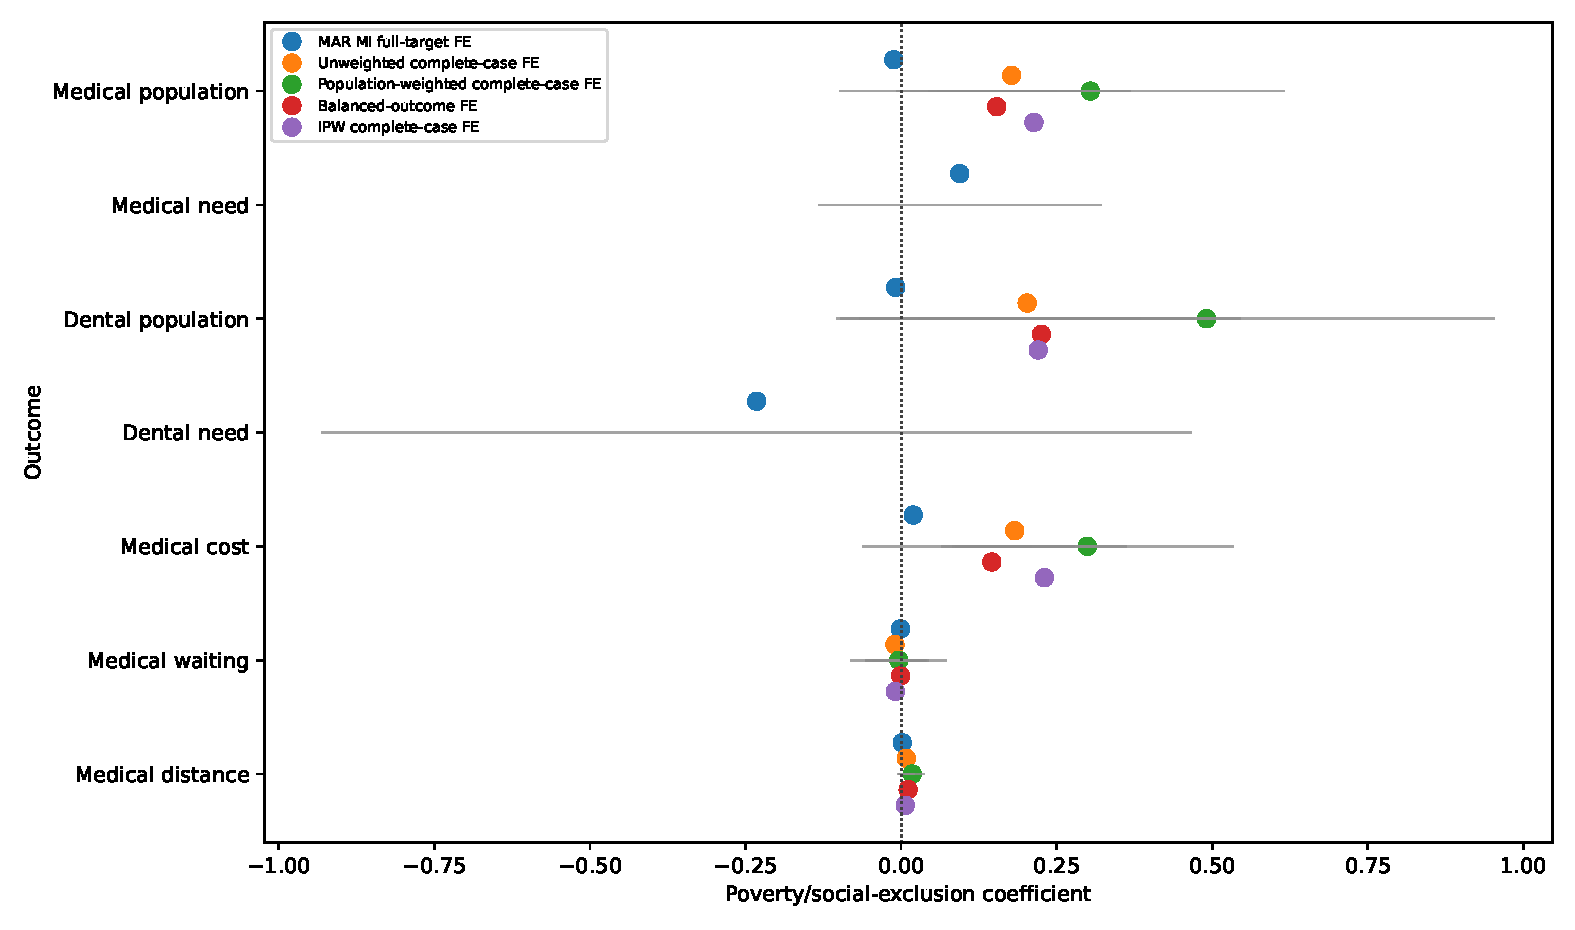
\includegraphics[width=0.94\textwidth]{outcome_estimand_coefficient_stability}
\caption{Coefficient stability across outcomes and estimands. Points show estimated poverty/social-exclusion coefficients for rows that meet the feasibility rule; horizontal intervals show 95\% confidence intervals. Infeasible estimands are omitted from the plot but retained in Table~\ref{tab:outcome_estimand_coefficient_matrix}.}
\label{fig:outcome_estimand_coefficient_stability}
\vspace{0.25em}

\begin{minipage}{0.94\textwidth}
\scriptsize \textit{Source:} Author's estimates from the outcome-by-estimand matrix. The figure is a stability diagnostic for aggregate coefficients, not evidence of individual-level effects.
\end{minipage}
\end{figure}

\begin{table}[H]
\centering
\caption{Drift-stability summary for the poverty/social-exclusion stress-test coefficient. The table reports framework metrics generated from the outcome-by-estimand matrix; TDI summarizes target movement and CSI summarizes conclusion agreement under the declared tolerance rule.}
\label{tab:drift_stability_summary}
\begingroup
\scriptsize
\setlength{\tabcolsep}{3pt}
\begin{tabularx}{\linewidth}{@{}p{0.15\linewidth}p{0.08\linewidth}rrrrrp{0.08\linewidth}p{0.16\linewidth}p{0.14\linewidth}@{}}
\toprule
Outcome & Denom. & Families & Median $\theta$ & $\theta$ IQR & Dir. agree & CSI & Median TDI & Label & Rule reason \\
\midrule
Dental population & population & 5 & 0.377 & 0.077 & 0.800 & 0.231 & 0.342 & missingness-dependent & CC--MI gap=0.365 \\
Medical cost & population & 5 & 1.133 & 0.466 & 1.000 & 0.000 & 0.343 & missingness-dependent & CC--MI gap=1.037 \\
Medical distance & population & 5 & 0.281 & 0.187 & 1.000 & 0.000 & 0.343 & missingness-dependent & CC--MI gap=0.225 \\
Medical population & population & 5 & 0.479 & 0.105 & 0.800 & 0.000 & 0.343 & missingness-dependent & CC--MI gap=0.512 \\
Medical waiting & population & 5 & -0.019 & 0.041 & 1.000 & 0.590 & 0.342 & target-dependent & CSI=0.590 and dir. agree=1.000 \\
Dental need & same\_needs & 1 & -0.309 & NA & NA & NA & 0.000 & non-identifiable & <2 estimand families \\
Medical need & same\_needs & 1 & 0.229 & NA & NA & NA & 0.000 & non-identifiable & <2 estimand families \\
\bottomrule
\end{tabularx}
\endgroup

\vspace{0.25em}

\begin{minipage}{0.96\textwidth}
\scriptsize \textit{Source:} Author's calculations from \texttt{target\_drift\_components.csv}, \texttt{drift\_stability\_theta.csv}, and \texttt{conclusion\_stability.csv}. Labels are deterministic diagnostics from the generated framework metrics; they are not causal or policy-effect classifications.
\end{minipage}
\end{table}

\section{Framework-Parameter Sensitivity}

The drift-stability labels depend on declared diagnostic choices, especially the CSI tolerance \(\delta\). Table~\ref{tab:framework_parameter_sensitivity_summary} varies \(\delta\) from 0.05 to 0.20 and recomputes the labels. It also recomputes TDI under equal, support-focused, and balance-focused component weights. These checks do not prove that the thresholds are optimal. They show whether the reported audit labels are fragile to declared diagnostic choices. Only medical waiting changes at the loosest \(\delta=0.20\); TDI weighting does not change labels because classification uses coefficient stability, complete-case--MI gaps, observed-estimand movement, and feasibility rules rather than a TDI cutoff.

\begin{table}[H]
\centering
\caption{Framework-parameter sensitivity of final labels. CSI columns vary the tolerance parameter \(\delta\); the TDI column reports whether equal, support-focused, or balance-focused TDI weights alter any target-dependent label.}
\label{tab:framework_parameter_sensitivity_summary}
\begingroup
\scriptsize
\setlength{\tabcolsep}{3pt}
\begin{tabularx}{\linewidth}{@{}p{0.12\linewidth}p{0.06\linewidth}p{0.14\linewidth}p{0.11\linewidth}p{0.11\linewidth}p{0.11\linewidth}p{0.11\linewidth}p{0.08\linewidth}p{0.08\linewidth}@{}}
\toprule
Outcome & Denom. & Baseline & $\delta=.05$ & $\delta=.10$ & $\delta=.15$ & $\delta=.20$ & CSI change? & TDI change? \\
\midrule
Dental pop. & pop. & miss.-dep. & miss.-dep. & miss.-dep. & miss.-dep. & miss.-dep. & No & No \\
Med. cost & pop. & miss.-dep. & miss.-dep. & miss.-dep. & miss.-dep. & miss.-dep. & No & No \\
Med. dist. & pop. & miss.-dep. & miss.-dep. & miss.-dep. & miss.-dep. & miss.-dep. & No & No \\
Med. pop. & pop. & miss.-dep. & miss.-dep. & miss.-dep. & miss.-dep. & miss.-dep. & No & No \\
Med. wait & pop. & target-dep. & target-dep. & target-dep. & target-dep. & stable & Yes & No \\
Dental need & need & non-ident. & non-ident. & non-ident. & non-ident. & non-ident. & No & No \\
Med. need & need & non-ident. & non-ident. & non-ident. & non-ident. & non-ident. & No & No \\
\bottomrule
\end{tabularx}
\endgroup

\vspace{0.25em}

\begin{minipage}{0.96\textwidth}
\scriptsize \textit{Source:} Author's calculations from the generated drift-stability matrix. Detailed CSI values and TDI-weighted summaries are stored in \texttt{outputs/framework\_parameter\_sensitivity.csv}.
\end{minipage}
\end{table}

\FloatBarrier

\section{Semi-Synthetic Missingness Simulation}

The simulation starts from the 282-row complete primary-outcome reference panel and estimates the poverty/social-exclusion reference estimand before imposing MCAR, early-year, country-group, financing-block, MAR-style, MNAR high-poverty/high-unmet, and Eurostat-realistic missingness. It then compares complete-case FE, population-weighted FE, IPW FE, PMM MI, and MNAR-shift MI. The exercise does not claim a definitive European coefficient; it tests how estimators behave when the complete artificial panel is known before deletion. Each draw also records the TDI components, coefficient error, sign reversal, interval coverage, wrong-conclusion rate, and failed replicates.

\begin{table}[H]
\centering
\scriptsize
\caption{Semi-synthetic missingness simulation summary. The reference estimand is the poverty/social-exclusion coefficient from the complete 282-row primary panel. Each mechanism uses 100 replicates; the table reports selected estimators to show bias, sign reversal, interval coverage of the reference estimand, and wrong-conclusion rates.}
\label{tab:simulation_main_summary}
\begin{tabular}{p{0.19\linewidth}p{0.18\linewidth}rrrrr}
\toprule
Mechanism & Estimator & Mean bias & Med. abs. error & Sign rev. & CI cov. & Wrong concl. \\
\midrule
Country group & CC FE & 0.0072 & 0.0271 & 0.0 & 1.0 & 0.0 \\
Country group & MNAR-shift MI & -0.1497 & 0.1476 & 0.15 & 0.01 & 0.15 \\
Country group & PMM MI & -0.1458 & 0.1466 & 0.12 & 0.02 & 0.12 \\
Covariate block & CC FE & -0.0048 & 0.0342 & 0.0 & 1.0 & 0.0 \\
Covariate block & MNAR-shift MI & -0.0028 & 0.0026 & 0.0 & 1.0 & 0.0 \\
Covariate block & PMM MI & -0.0026 & 0.0025 & 0.0 & 1.0 & 0.0 \\
Early-year & CC FE & -0.0773 & 0.0773 & 0.0 & 1.0 & 0.0 \\
Early-year & MNAR-shift MI & -0.2299 & 0.2303 & 1.0 & 0.0 & 1.0 \\
Early-year & PMM MI & -0.2304 & 0.2316 & 1.0 & 0.0 & 1.0 \\
Eurostat-realistic & CC FE & -0.0156 & 0.0439 & 0.0 & 0.94 & 0.0 \\
Eurostat-realistic & MNAR-shift MI & -0.0857 & 0.0879 & 0.0 & 0.46 & 0.0 \\
Eurostat-realistic & PMM MI & -0.0603 & 0.0612 & 0.0 & 0.79 & 0.0 \\
MAR observed & CC FE & -0.0019 & 0.0274 & 0.0 & 1.0 & 0.0 \\
MAR observed & MNAR-shift MI & -0.1471 & 0.1464 & 0.07 & 0.01 & 0.07 \\
MAR observed & PMM MI & -0.1419 & 0.1422 & 0.06 & 0.02 & 0.06 \\
MCAR & CC FE & 0.0028 & 0.1212 & 0.15 & 0.89 & 0.15 \\
MCAR & MNAR-shift MI & -0.1448 & 0.1434 & 0.05 & 0.0 & 0.05 \\
MCAR & PMM MI & -0.1315 & 0.1337 & 0.0 & 0.01 & 0.0 \\
MNAR high-pov./unmet & CC FE & -0.0164 & 0.0329 & 0.0 & 0.95 & 0.0 \\
MNAR high-pov./unmet & MNAR-shift MI & -0.1427 & 0.14 & 0.07 & 0.0 & 0.07 \\
MNAR high-pov./unmet & PMM MI & -0.1483 & 0.1484 & 0.12 & 0.01 & 0.12 \\
\bottomrule
\end{tabular}

\vspace{0.25em}

\begin{minipage}{0.96\textwidth}
\scriptsize \textit{Source:} Author's semi-synthetic simulation based on the complete-case Eurostat primary panel. The full validation output is generated in \texttt{outputs/simulation\_validation\_summary.csv}; the reference estimand is defined inside the simulation and is not a claim about a true European causal coefficient.
\end{minipage}
\end{table}

Table~\ref{tab:simulation_main_summary} shows that the direction of failure depends on the missingness mechanism. Complete-case FE is relatively stable under country-group, covariate-block, MAR-style, and Eurostat-realistic deletion in this reference panel, but MCAR deletion can create sign reversals because retained rows become small and noisy. PMM MI and MNAR-shift MI are not uniformly better. Figure~\ref{fig:simulation_tdi_validation_combined} links the simulation back to the framework: larger diagnostic drift is not a theorem of bias, but the generated draws show why target definition, row loss, estimator sensitivity, and non-identifiability should be reported before interpreting substantive coefficients.

\begin{figure}[H]
\centering
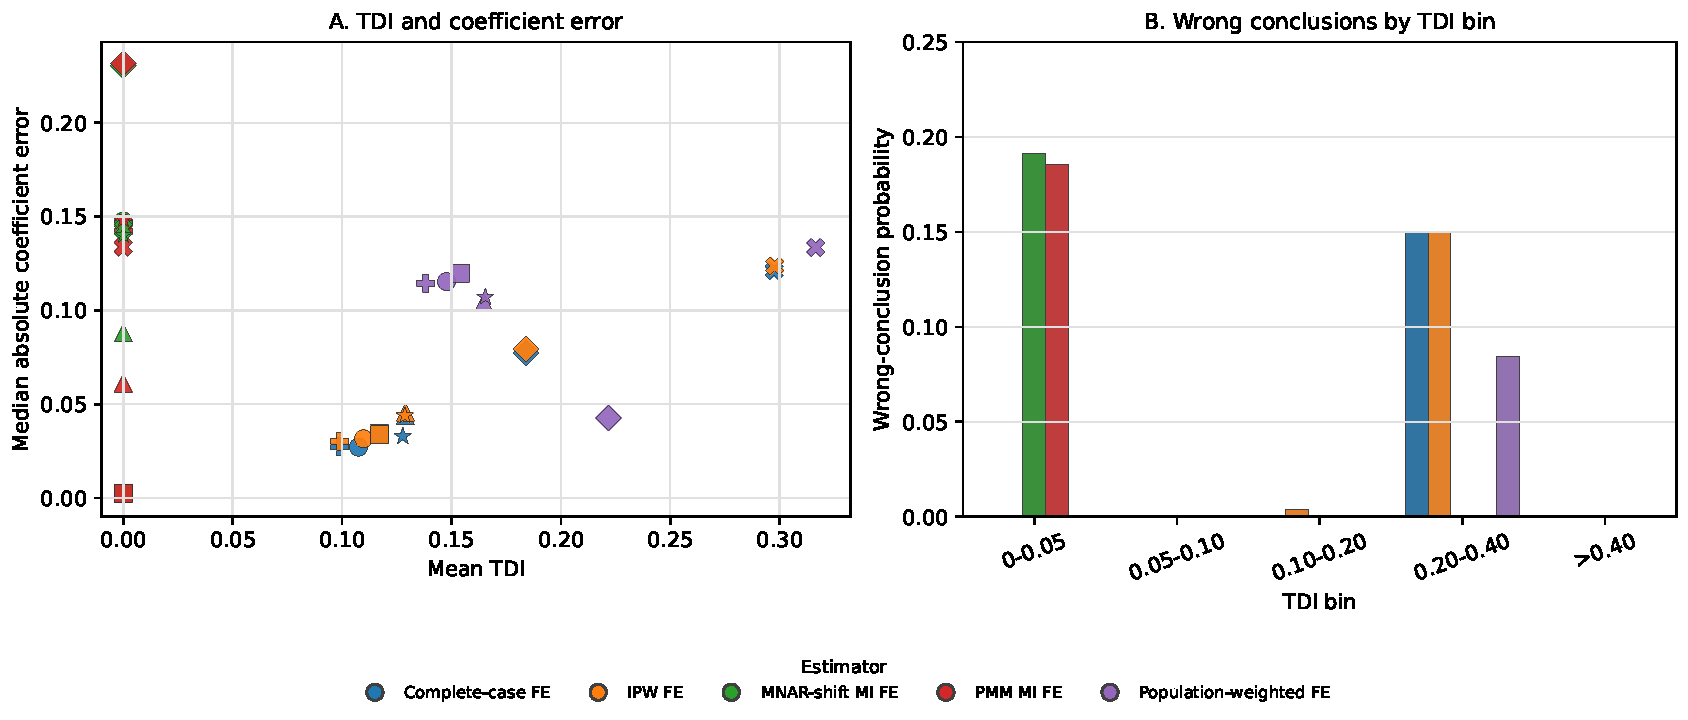
\includegraphics[width=0.98\textwidth]{simulation_tdi_validation_combined}
\caption{TDI validation diagnostics in the semi-synthetic simulation. Panel A compares mean TDI with median absolute coefficient error by mechanism--estimator cell. Panel B compares wrong-conclusion probability across TDI bins.}
\label{fig:simulation_tdi_validation_combined}
\vspace{0.25em}

\begin{minipage}{0.94\textwidth}
\scriptsize \textit{Source:} Author's semi-synthetic missingness simulation. TDI is used as an audit diagnostic; the figure does not claim that TDI proves bias.
\end{minipage}
\end{figure}

\begin{table}[htbp]
\centering
\small
\caption{Conceptual role of variable blocks in the aggregate panel. The table organizes interpretation for country-year associations and does not identify intervention effects.}
\label{tab:conceptual_variable_roles}
\begin{tabular}{@{}p{0.24\textwidth}p{0.30\textwidth}p{0.36\textwidth}@{}}
\toprule
Block & Variables & Role in interpretation \\
\midrule
Social vulnerability & Poverty or social exclusion, unemployment, inequality & Main associational exposure block; not individual-level risk. \\
Macroeconomic context & GDP per capita, GDP growth & Country-year resource context and confounding proxy. \\
Health-system financing & Government expenditure, compulsory financing, OOP share & Affordability and institutional proxies; not direct intervention estimates. \\
Capacity & Physicians and hospital beds & Availability proxies, mostly for prediction and sensitivity. \\
Country and year structure & Country indicators, year indicators & Persistent national differences and common period shocks. \\
Missingness selection & Inclusion probability, coverage flags, imputation predictors & Data-availability process that changes the analytical target. \\
\bottomrule
\end{tabular}
\vspace{0.25em}

\begin{minipage}{0.94\textwidth}
\scriptsize \textit{Source:} Author's synthesis from Chapter~\ref{ch:background_literature} and the variables in Table~\ref{tab:variable_summary}. The table defines interpretation roles for the aggregate model.
\end{minipage}
\end{table}

This conceptual table is not a causal identification graph. It clarifies why the same coefficient can change when the row set, adjustment block, or missing-data assumption changes; ecological aggregation still prevents individual-level interpretation \citep{robinson_1950,greenland_morgenstern_1989}.

\section{Complete-Case Selection}

The intended monitoring target contains 608 country-years with observed unmet medical care need. The selected fixed-effects regression sample contains 282 country-years complete for the baseline covariates. Table~\ref{tab:complete_case_selection_model} therefore comes before the baseline regression: it diagnoses how the analytical row set is formed.

The selection model is not causal. It asks whether inclusion in the complete-case regression is related to observed unmet need and observed macro conditions. Country-group terms are included in the diagnostic model but omitted from the compact displayed table. Predictable inclusion means the complete-case coefficient should be read as a selected-panel estimand, not as the coefficient for the full outcome-observed monitoring target.

\begin{table}[H]
\centering
\small
\caption{Complete-case inclusion model. The diagnostic uses all 608 outcome-observed country-years to model inclusion in the 282-row baseline complete-case regression sample; it is unweighted and country-clustered.}
\label{tab:complete_case_selection_model}
\begin{tabular}{@{}lrrr@{}}
\toprule
Predictor & Coef. & SE & p-value \\
\midrule
Unmet need & -0.000 & 0.007 & 0.951 \\
Log GDP & 0.145 & 0.070 & 0.038 \\
Unemployment & -0.016 & 0.006 & 0.009 \\
GDP missing & -0.524 & 0.135 & <0.001 \\
Unemployment missing & -0.279 & 0.049 & <0.001 \\
Year & 0.036 & 0.005 & <0.001 \\
\bottomrule
\end{tabular}

\vspace{0.2em}
\begin{minipage}{0.92\textwidth}\scriptsize Notes: Linear probability model for inclusion in the baseline complete-case regression sample among the 608 outcome-observed rows, with country-clustered standard errors. GDP and unemployment are median-imputed for this diagnostic and accompanied by missingness indicators.\end{minipage}

\vspace{0.25em}

\begin{minipage}{0.92\textwidth}
\scriptsize \textit{Source:} Author's calculations from the outcome-observed Eurostat primary panel. The model is a selection diagnostic following missing-data reporting logic \citep{little_rubin_2019,seaman_white_2013}.
\end{minipage}
\end{table}

\begin{figure}[H]
\centering
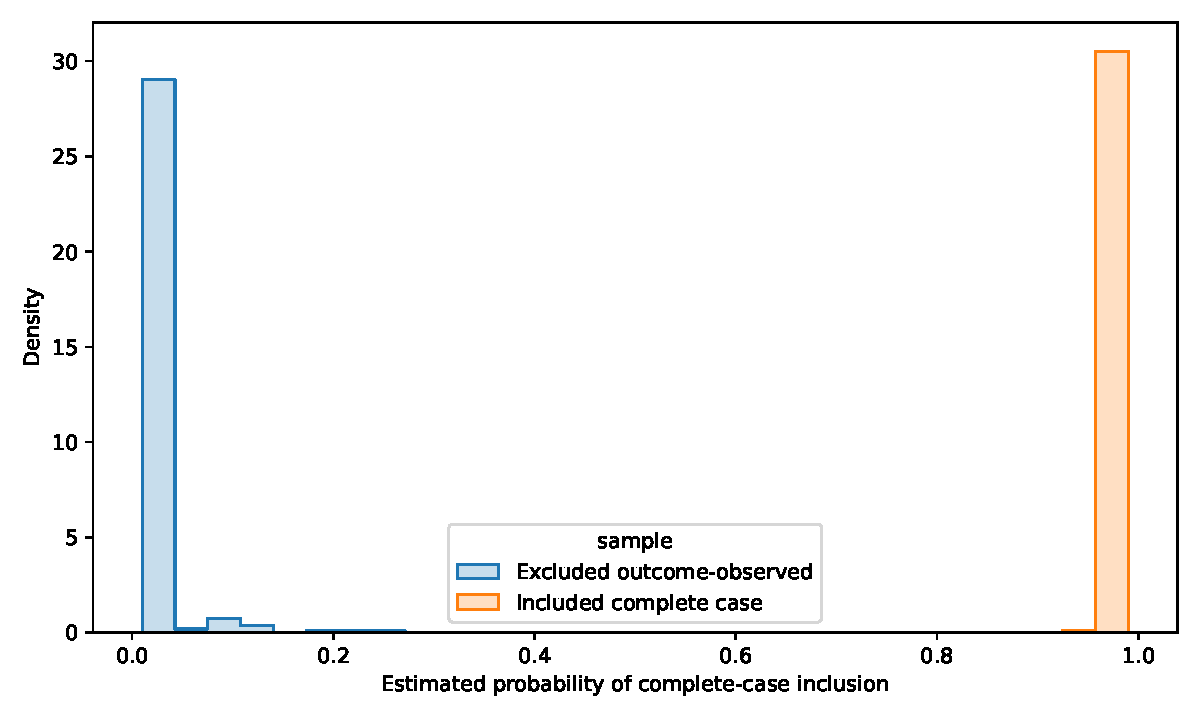
\includegraphics[width=0.82\textwidth]{missingness_inclusion_probability}
\caption{Estimated probability of complete-case inclusion among the 608 outcome-observed country-years. The figure compares rows included in the 282-row baseline complete-case FE model with outcome-observed rows excluded because covariates are missing.}
\label{fig:missingness_inclusion_probability}
\vspace{0.25em}

\begin{minipage}{0.9\textwidth}
\scriptsize \textit{Source:} Author's predictions from the complete-case inclusion model in Table~\ref{tab:complete_case_selection_model}.
\end{minipage}
\end{figure}

\FloatBarrier

\section{Selected Complete-Case Baseline}

The pooled specification relates unmet medical care need in country \(i\) and year \(t\) to country-year covariates and year indicators:
\[
y_{it} = \alpha + X_{it}\beta + \lambda_t + \varepsilon_{it}.
\]
The main fixed-effects specification adds country indicators:
\[
y_{it} = \alpha_i + X_{it}\beta + \lambda_t + \varepsilon_{it}.
\]
Both pooled and two-way fixed-effects models report country-clustered standard errors with a finite-sample correction, reflecting repeated observations within countries \citep{arellano_1987,bertrand_duflo_mullainathan_2004}.

\begin{table}[htbp]
\centering
\small
\caption{Baseline regression estimates for unmet medical care need. The FE column is the selected 282-row complete-case country-year sample over 2015--2024 with country and year fixed effects and country-clustered standard errors.}
\label{tab:regression_main_results}
\begin{tabular}{lcc}
\toprule
Variable & Pooled + year & Country + year \\
\midrule
Log GDP per capita & -0.546 (0.593) & -1.041 (2.201) \\
Unemployment rate & 0.160 (0.186) & -0.034 (0.087) \\
Poverty or social exclusion & 0.062 (0.065) & 0.177 (0.067) \\
Government health expenditure & 0.159 (0.190) & -0.229 (0.446) \\
Compulsory health financing & -0.401 (0.243) & 0.097 (0.444) \\
\midrule
Observations & 282 & 282 \\
Countries & 30 & 30 \\
Year indicators & Yes & Yes \\
Country indicators & No & Yes \\
$R^2$ & 0.221 & 0.895 \\
\bottomrule
\end{tabular}

\vspace{0.2em}
\begin{minipage}{0.92\textwidth}
\scriptsize Notes: Cells report coefficient estimates with standard errors in parentheses. Both the pooled model and the country-and-year fixed-effects model use country-clustered standard errors with finite-sample correction. No star thresholds are used because the thesis emphasizes coefficient stability across estimands.
\end{minipage}

\vspace{0.25em}

\begin{minipage}{0.92\textwidth}
\scriptsize \textit{Source:} Author's estimates from the 282-row complete-case Eurostat panel. The table is the selected-panel baseline used for later sensitivity comparisons.
\end{minipage}
\end{table}

The baseline country-and-year fixed-effects model gives a positive poverty/social-exclusion coefficient in the selected complete-case panel. This is the starting point, not the thesis conclusion. It uses 282 rows from 30 countries, while the outcome-observed monitoring target has 608 rows from 37 countries.

\section{Reduced-Covariate Model Ladder}

Before moving to IPW and imputation, Table~\ref{tab:model_ladder_results} asks whether the poverty/social-exclusion coefficient changes because of adjustment choices, country-universe restriction, population weighting, or balanced-outcome coverage. Models A--F are estimated with country and year fixed effects where feasible. The ladder starts with poverty only, then adds macroeconomic context, health financing, capacity, and broader theory-driven controls. The final reduced high-coverage model keeps the social-vulnerability and macro-labour structure while avoiding the larger coverage cost of system-expanded covariates.

\begin{table}[htbp]
\centering
\caption{Reduced-covariate model ladder for the poverty/social-exclusion coefficient. Rows report country-and-year FE estimates where feasible; infeasible rows are retained rather than forced.}
\label{tab:model_ladder_results}
\begingroup
\scriptsize
\setlength{\tabcolsep}{3pt}
\renewcommand{\arraystretch}{1.12}
\begin{tabularx}{\textwidth}{@{}p{0.26\textwidth}Yrrrp{0.20\textwidth}l@{}}
\toprule
Spec. & Target/weighting & Rows & Countries & Years & Coef. [95\% CI] & p-value \\
\midrule
A: Poverty only & Full available; unweighted & 375 & 36 & 11 & 0.157 [0.050, 0.264] & 0.004 \\
B: Poverty + GDP + unemployment & Full available; unweighted & 360 & 34 & 11 & 0.127 [0.009, 0.244] & 0.035 \\
C: B + health financing & Full available; unweighted & 282 & 30 & 10 & 0.178 [0.046, 0.309] & 0.008 \\
D: C + capacity & Full available; unweighted & 233 & 27 & 9 & 0.112 [-0.048, 0.272] & 0.171 \\
E: Full theory model & Full available; unweighted & 231 & 27 & 9 & 0.108 [-0.053, 0.268] & 0.189 \\
F: Reduced high-coverage model & Full available; unweighted & 358 & 34 & 11 & 0.132 [0.014, 0.249] & 0.028 \\
C-EU27: EU-27 baseline & EU-27; unweighted & 258 & 27 & 10 & 0.179 [0.034, 0.324] & 0.015 \\
C-PW: Population-weighted baseline & Full available; population-weighted & 282 & 30 & 10 & 0.304 [-0.007, 0.615] & 0.055 \\
C-BO: Balanced-outcome baseline & Balanced outcome; unweighted & 238 & 25 & 10 & 0.154 [0.060, 0.248] & 0.001 \\
C-BO-PW: Balanced-outcome weighted & Balanced outcome; population-weighted & 238 & 25 & 10 & 0.147 [-0.026, 0.320] & 0.096 \\
\bottomrule
\end{tabularx}

\vspace{0.2em}
\begin{minipage}{0.94\textwidth}\scriptsize Notes: All rows use country-and-year fixed effects and country-clustered standard errors. The ladder separates covariate adjustment from sample loss: A--F add or remove covariate blocks, C-EU27 changes country universe, C-PW changes weighting, and C-BO rows restrict to the balanced-outcome country set. Population weights are year-normalized country populations.\end{minipage}
\endgroup

\vspace{0.25em}

\begin{minipage}{0.96\textwidth}
\scriptsize \textit{Source:} Author's estimates from the Eurostat panel. Each row changes covariate set, weighting, country universe, or coverage restriction, so the table diagnoses coefficient stability across estimands.
\end{minipage}
\end{table}

\begin{figure}[htbp]
\centering
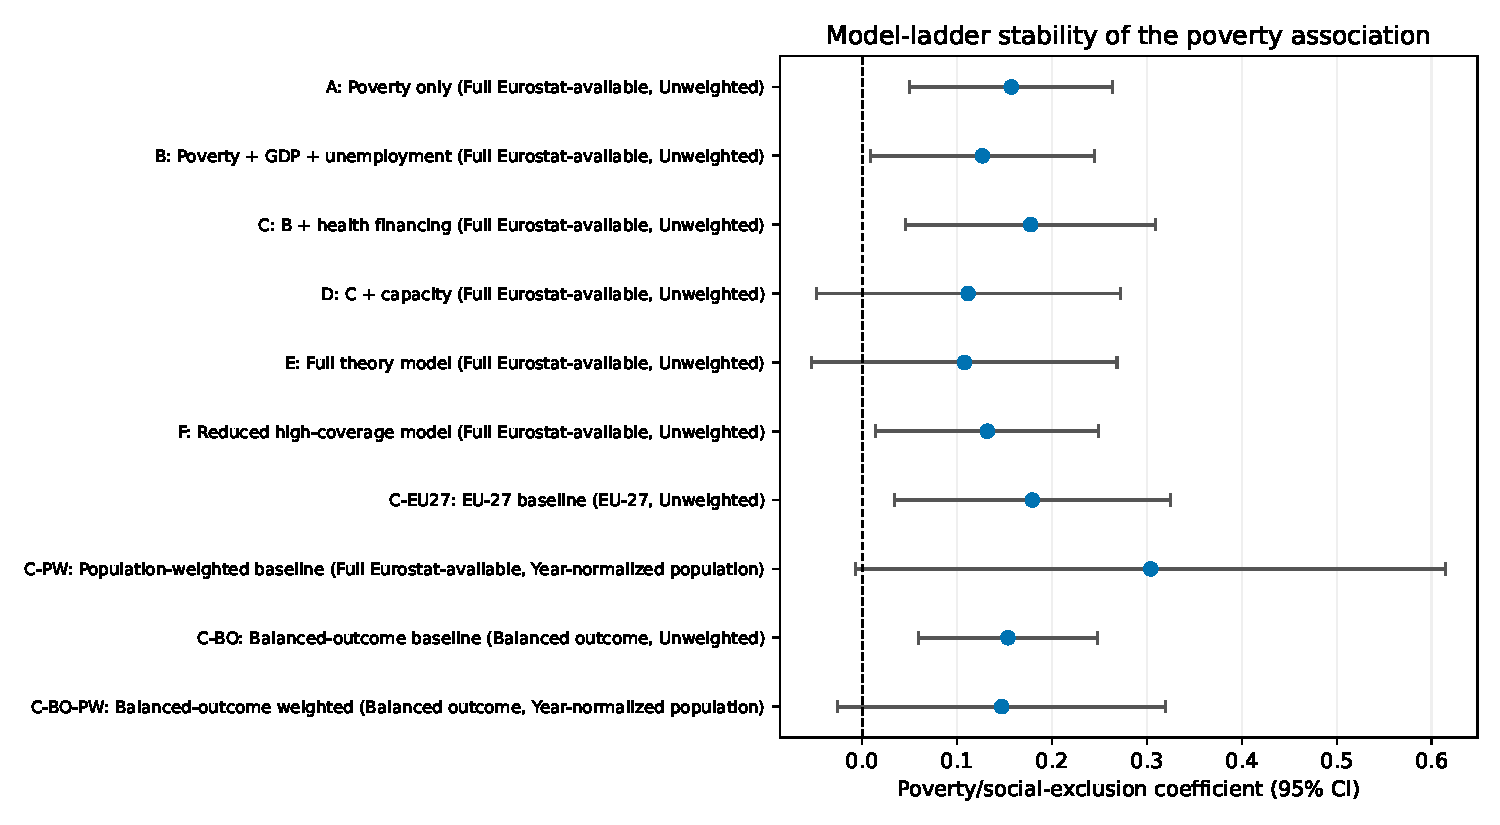
\includegraphics[width=0.92\textwidth]{model_ladder_coefficient_forest}
\caption{Coefficient stability across the model ladder. Points show the poverty/social-exclusion coefficient and 95\% confidence interval for feasible country-and-year FE specifications; rows differ by covariate set, weighting, country universe, or balanced-outcome restriction.}
\label{fig:model_ladder_coefficient_forest}
\vspace{0.25em}

\begin{minipage}{0.94\textwidth}
\scriptsize \textit{Source:} Author's estimates from Table~\ref{tab:model_ladder_results}. The plot visualizes how the same stress-test coefficient moves across model and target definitions.
\end{minipage}
\end{figure}

The model ladder separates three sources of movement. First, adding macroeconomic and financing variables changes the coefficient while also changing the retained country-year sample. Second, population weighting changes the monitoring question from equal-country to resident-weighted interpretation. Third, the EU-27 row tests whether the main selected-panel association is specific to the broader Eurostat-available country universe. These are estimand changes, not minor technical variants.

\section{Sensitivity Ladder}

Table~\ref{tab:main_sensitivity_ladder} is the main result table. It follows the poverty/social-exclusion coefficient across the model hierarchy, population weighting, balanced-outcome restriction, country-universe restrictions, lagged covariates, measurement-period checks, crisis-period exclusion, conservative country trends, IPW, MAR MI, and MNAR delta-shift sensitivity. Specifications with too few rows, countries, or years are reported as infeasible instead of forced.

The ladder shows the central empirical pattern. Observed covariate-complete specifications often remain positive, especially the country-and-year FE, balanced-outcome, EU-27, and IPW rows. The lagged-covariate, 2015-exclusion, and country-trend rows weaken precision. The MAR and MNAR imputation rows move the estimand to the full outcome-observed target and attenuate the poverty coefficient toward zero. The coefficient is therefore not a property of ``Europe'' in general; it is a property of a defined estimand.

The EU-27 row is close to the full Eurostat-available complete-case estimate, while smaller EEA and candidate-country universes are not large enough for stable fixed-effects inference. This supports the interpretation that the main difference is not EU-27 versus full operational Europe, but selected complete cases versus broader outcome-observed targets.

\begin{table}[H]
\centering
\scriptsize
\caption{Main sensitivity ladder for the poverty/social-exclusion coefficient. Rows use the generated thesis pipeline and distinguish model hierarchy, target population, universe, weighting, selection adjustment, and imputation assumptions.}
\label{tab:main_sensitivity_ladder}
\resizebox{\textwidth}{!}{%
\begin{tabular}{@{}p{0.18\textwidth}p{0.23\textwidth}rrp{0.16\textwidth}p{0.22\textwidth}@{}}
\toprule
Step & Target & Countries & Rows & Coef. [95\% CI] & Interpretation \\
\midrule
Pooled complete-case & selected complete-case rows & 30 & 282 & 0.062 [-0.065, 0.189] & associational baseline before country FE \\
Country FE & selected complete-case rows & 30 & 282 & 0.234 [0.118, 0.351] & absorbs persistent country differences \\
Country + year FE & selected complete-case rows & 30 & 282 & 0.178 [0.046, 0.309] & selected-panel primary FE estimate \\
Population-weighted FE & selected complete-case rows & 30 & 282 & 0.304 [-0.007, 0.615] & resident-weighted selected-panel estimand \\
Balanced-outcome FE & balanced outcome/population country set & 25 & 238 & 0.154 [0.060, 0.248] & coverage-restricted monitoring target \\
Full Eurostat-available FE & full Eurostat-available complete-case rows & 30 & 282 & 0.178 [0.046, 0.309] & full operational Europe universe \\
EU-27 FE & EU-27 complete-case rows & 27 & 258 & 0.179 [0.034, 0.324] & EU institutional universe sensitivity \\
Extended Europe FE & extended europe complete-case rows & 30 & 282 & 0.178 [0.046, 0.309] & additional country-universe sensitivity \\
EEA-country FE & eea-country complete-case rows & 2 & 14 & not estimated & additional country-universe sensitivity \\
Candidate FE & candidate complete-case rows & 0 & 0 & not estimated & additional country-universe sensitivity \\
Lagged covariates & outcome-observed rows with lag-complete covariates & 30 & 280 & 0.074 [-0.035, 0.182] & temporal-ordering check \\
Excluding 2015 & selected complete-case rows excluding 2015 & 30 & 252 & 0.099 [-0.018, 0.216] & measurement-break diagnostic \\
Excluding COVID years & selected complete-case rows excluding 2020--2022 & 30 & 195 & 0.230 [0.064, 0.396] & crisis-period sensitivity \\
Country trends & selected complete-case rows & 30 & 282 & 0.125 [-0.027, 0.278] & conservative over-control sensitivity \\
IPW & selected complete-case rows & 30 & 282 & 0.178 [0.046, 0.310] & selection diagnostic, not structural correction \\
MAR MI & 608 outcome-observed rows & 37 & 608 & 0.014 [-0.071, 0.099] & model-based broader target \\
MNAR pessimistic & 608 outcome-observed rows & 37 & 608 & 0.010 [-0.086, 0.107] & missing rows shifted toward worse macro-social conditions \\
MNAR optimistic & 608 outcome-observed rows & 37 & 608 & 0.010 [-0.086, 0.106] & missing rows shifted toward less severe macro-social conditions \\
\bottomrule
\end{tabular}%
}

\vspace{0.2em}
\begin{minipage}{0.96\textwidth}\scriptsize Notes: The ladder follows the poverty/social-exclusion coefficient as the model, country universe, weighting rule, selection adjustment, and imputation assumption change. Infeasible rows are retained when fixed-effects estimation has too few rows, countries, or years. MAR and MNAR rows are model-based sensitivity estimands, not corrected truth.\end{minipage}

\vspace{0.25em}

\begin{minipage}{0.96\textwidth}
\scriptsize \textit{Source:} Author's estimates from the thesis regression, IPW, MAR MI, and MNAR sensitivity pipeline. Observed-data FE rows use country-clustered uncertainty; imputed rows are pooled sensitivity estimands.
\end{minipage}
\end{table}

\begin{table}[H]
\centering
\small
\caption{Country-universe sensitivity for the poverty association. Rows use unweighted country-and-year fixed-effects models on available covariate-complete rows within each country universe; infeasible rows are reported rather than forced.}
\label{tab:universe_sensitivity_results}
\begingroup
\small
\begin{tabular}{@{}lrrll@{}}
\toprule
Universe & Countries & Rows & Coef. [95\% CI] & Status \\
\midrule
Full & 30 & 282 & 0.178 [0.046, 0.309] & estimated \\
EU-27 & 27 & 258 & 0.179 [0.034, 0.324] & estimated \\
EEA countries & 2 & 14 &  & infeasible (<50 rows) \\
Extended & 30 & 282 & 0.178 [0.046, 0.309] & estimated \\
Candidates & 0 & 0 &  & infeasible (<50 rows) \\
\bottomrule
\end{tabular}

\vspace{0.2em}
\begin{minipage}{0.92\textwidth}\scriptsize Notes: Rows report the poverty/social-exclusion coefficient from unweighted country-and-year fixed-effects models estimated on available covariate-complete rows within each country universe. Infeasible rows are not forced when the universe has too few complete-case countries, years, or rows.\end{minipage}
\endgroup

\vspace{0.25em}

\begin{minipage}{0.92\textwidth}
\scriptsize \textit{Source:} Author's estimates from country-universe filters defined in Chapter~\ref{ch:data_indicators}. Infeasible rows are retained to show support limits.
\end{minipage}
\end{table}

\FloatBarrier

\section{Inference Diagnostics}

The selected complete-case coefficient is also checked against alternative inference treatments. Table~\ref{tab:fe_inference_comparison} compares country-clustered, Driscoll--Kraay, and wild-cluster bootstrap inference for the same 282-row country-and-year FE estimand.

\begin{table}[htbp]
\centering
\small
\caption{Inference diagnostics for the selected complete-case poverty coefficient. The table compares country-clustered, Driscoll--Kraay, and wild-cluster bootstrap inference for the same 282-row country-and-year FE estimand.}
\label{tab:fe_inference_comparison}
\begin{tabular}{@{}lrrrrr@{}}
\toprule
Term & Coef. & Cluster SE & DK SE & Wild \(p\) & Wild 95\% CI \\
\midrule
Poverty/social exclusion & 0.178 & 0.067 & 0.076 & 0.004 & [0.058, 0.297] \\
\bottomrule
\end{tabular}

\vspace{0.2em}
\begin{minipage}{0.94\textwidth}\scriptsize Notes: The coefficient is from the selected complete-case country-and-year fixed-effects model. Cluster SE uses country clusters with finite-sample correction; DK is Driscoll--Kraay with one lag; the wild-cluster bootstrap uses country-level Rademacher weights and reports the bootstrap \(p\)-value and percentile interval.\end{minipage}

\vspace{0.25em}

\begin{minipage}{0.94\textwidth}
\scriptsize \textit{Source:} Author's inference diagnostics for the selected complete-case FE model. The comparison addresses dependence and small-cluster sensitivity but does not alter the target population.
\end{minipage}
\end{table}

\begin{table}[htbp]
\centering
\small
\caption{Fit diagnostics for the selected complete-case FE model. The table foregrounds within-\(R^2\), country count, year coverage, and years per country so the absorbed country/year structure is not mistaken for explanatory power of the time-varying covariates.}
\label{tab:fe_fit_diagnostics}
\resizebox{\textwidth}{!}{%
\begin{tabular}{@{}lrrrrrrrrr@{}}
\toprule
Model & \(N\) & Countries & Years & Avg. years & Min years & Max years & Within \(R^2\) & Between \(R^2\) & Overall \(R^2\) \\
\midrule
Baseline FE & 282 & 30 & 10 & 9.4 & 6 & 10 & 0.098 & 0.229 & 0.895 \\
\bottomrule
\end{tabular}%
}

\vspace{0.2em}
\begin{minipage}{0.94\textwidth}\scriptsize Notes: The baseline fixed-effects sample is the complete-case panel used for the selected poverty coefficient. The within \(R^2\) is emphasized because country and year effects absorb much of the overall variation.\end{minipage}

\vspace{0.25em}

\begin{minipage}{0.94\textwidth}
\scriptsize \textit{Source:} Author's diagnostics from the baseline complete-case FE fit.
\end{minipage}
\end{table}

These diagnostics strengthen the presentation of the selected-panel estimate without changing its interpretation. The high overall \(R^2\) mostly reflects country and year indicators; within-\(R^2\) is much smaller. Robust inference diagnostics address serial dependence and the small number of country clusters, but they do not solve target-population drift.

\section{IPW Diagnostic}

IPW is retained as a diagnostic, not as a fix for structural Eurostat non-coverage \citep{seaman_white_2013}. The weights are estimated from observed unmet need, year, country group, macro conditions, missingness indicators, and coverage flags, then stabilized and truncated. In this dataset IPW changes little because the complete-case sample is selected mainly through structural covariate availability. Reweighting observed complete cases cannot recover rows where required covariates are absent.

\begin{table}[H]
\centering
\small
\caption{Missingness-aware comparison of the poverty association. Complete-case and IPW rows use the selected FE sample with country-clustered SE; MI rows pool estimates over imputed outcome-observed panels.}
\label{tab:missingness_robustness_results}
\begin{tabular}{@{}lrrrr@{}}
\toprule
Specification & Coef. & SE & p-value & \(N\) \\
\midrule
Complete-case two-way FE & 0.1775 & 0.0672 & 0.008 & 282 \\
Population-weighted complete-case FE & 0.3041 & 0.1585 & 0.055 & 282 \\
Earlier MI sensitivity & 0.0001 & 0.0012 & 0.899 & 422 \\
IPW two-way FE & 0.1782 & 0.0674 & 0.008 & 282 \\
PMM MI full target & 0.0139 & 0.0434 & 0.748 & 608 \\
\bottomrule
\end{tabular}

\vspace{0.2em}
\begin{minipage}{0.92\textwidth}
\scriptsize Notes: All rows report the poverty or social exclusion coefficient from country-and-year fixed-effects models. Complete-case and IPW rows use country-clustered standard errors. IPW weights are stabilized and truncated at the 1st and 99th percentiles. The improved multiple-imputation row pools 30 imputed full outcome-observed panels using Rubin's rules.
\end{minipage}

\vspace{0.25em}

\begin{minipage}{0.92\textwidth}
\scriptsize \textit{Source:} Author's estimates from the missingness-robustness pipeline. The table contrasts selected complete cases, IPW diagnostics, and MI sensitivity targets.
\end{minipage}
\end{table}

Population-weighted estimates use country-year total population from Eurostat \texttt{demo\_pjan}, normalized within year. They answer a resident-weighted monitoring question, not a universally more correct version of the country-weighted question.

\clearpage

\begin{table}[H]
\centering
\scriptsize
\caption{Target-population sensitivity of the poverty association. Rows compare unweighted, year-normalized population-weighted, balanced-outcome, and MI full-target estimands; complete-case rows use country-clustered FE estimates.}
\label{tab:target_population_sensitivity_results}
\resizebox{\textwidth}{!}{%
\begin{tabular}{@{}lllcrrp{0.22\textwidth}lp{0.17\textwidth}@{}}
\toprule
Spec. & Universe & Target & Weight & Countries & Rows & Coef. [95\% CI] & p-value & Reading \\
\midrule
CC & Full available & Selected CC & Unweighted & 30 & 282 & 0.178 [0.046, 0.309] & 0.008 & selected panel \\
EU-27 CC & EU-27 & Selected CC & Unweighted & 27 & 258 & 0.179 [0.034, 0.324] & 0.015 & EU-27 selected panel \\
CC pop. & Full available & Selected CC & Population & 30 & 282 & 0.304 [-0.007, 0.615] & 0.055 & selected resident-weighted \\
Balanced & Full available & Balanced outcome & Unweighted & 25 & 238 & 0.154 [0.060, 0.248] & 0.001 & observed-panel restriction \\
Balanced pop. & Full available & Balanced outcome & Population & 25 & 238 & 0.147 [-0.026, 0.320] & 0.096 & weighted restriction \\
MI full & Full available & Full observed & Unweighted & 37 & 608 & 0.014 [-0.071, 0.099] & 0.748 & model-based sensitivity \\
\bottomrule
\end{tabular}%
}

\vspace{0.2em}
\begin{minipage}{0.96\textwidth}\scriptsize Notes: The coefficient is for poverty or social exclusion in country-and-year fixed-effects models with country-clustered standard errors, except the MI row, which pools fixed-effects estimates using Rubin's rules. Full available means all Eurostat-available national units in the outcome-observed panel; EU-27 restricts to current EU member states. Population weights are country-year total population from \texttt{demo\_pjan}, normalized within year.\end{minipage}

\vspace{0.25em}

\begin{minipage}{0.96\textwidth}
\scriptsize \textit{Source:} Author's estimates from the Eurostat panel and \texttt{demo\_pjan}. The rows change the target population or weighting rule and therefore change the estimand being interpreted.
\end{minipage}
\end{table}

\clearpage

\section{MAR Multiple Imputation}

The MAR MI analysis asks whether the selected complete-case poverty coefficient survives when the target is broadened to the 608 outcome-observed rows under a bounded imputation design \citep{rubin_1987,little_rubin_2019}. The implementation uses predictive mean matching: missing covariate values are filled by donor values selected from observed cases with similar model-predicted values. Raw GDP and log GDP are not imputed independently; GDP per capita is derived from imputed log GDP when the raw value is missing.

\begin{table}[htbp]
\centering
\scriptsize
\caption{Baseline PMM diagnostics for imputed covariates. Diagnostics refer to the 608-row outcome-observed target, the 30-imputation baseline PMM model, and bounded plausible ranges for imputed covariates.}
\label{tab:mi_diagnostics_summary}
\resizebox{\textwidth}{!}{%
\begin{tabular}{@{}lrrrrr@{}}
\toprule
Variable & Missing & Bounds & Viol. & Obs. mean & Imp. mean \\
\midrule
Log GDP & 0.7\% & [7.0, 12.3] & 0 & 10.07 & 9.67 \\
Unemployment & 8.6\% & [0.0, 40.0] & 0 & 8.65 & 7.53 \\
Poverty/social exclusion & 38.3\% & [0.0, 60.0] & 0 & 22.83 & 24.81 \\
Government health expenditure & 17.4\% & [0.0, 15.0] & 0 & 6.28 & 5.58 \\
Compulsory financing & 27.0\% & [0.0, 15.0] & 0 & 6.52 & 5.55 \\
Gini & 32.7\% & [0.0, 60.0] & 0 & 30.26 & 30.29 \\
Physicians & 29.1\% & [0.0, 1000.0] & 0 & 358.74 & 355.50 \\
Hospital beds & 14.1\% & [0.0, 1500.0] & 0 & 488.33 & 480.61 \\
OOP share & 27.0\% & [0.0, 60.0] & 0 & 20.65 & 25.87 \\
Long-term unemployment & 8.9\% & [0.0, 30.0] & 0 & 3.85 & 3.33 \\
\bottomrule
\end{tabular}%
}

\vspace{0.2em}
\begin{minipage}{0.96\textwidth}\scriptsize Notes: Diagnostics refer to the baseline 30-imputation model over the 608 outcome-observed country-years. Bounds are the plausible ranges imposed before fitting the fixed-effects model. Viol. counts imputed values outside those bounds after clipping and should be zero.\end{minipage}

\vspace{0.25em}

\begin{minipage}{0.96\textwidth}
\scriptsize \textit{Source:} Author's MI diagnostics from the 608-row outcome-observed Eurostat target. The table reports plausibility checks for the imputation design, not substantive effects.
\end{minipage}
\end{table}

\begin{table}[htbp]
\centering
\small
\caption{Multiple-imputation sensitivity variants. Rows compare PMM variants with outcome inclusion, no-outcome specification, country indicators, lagged predictors, and a 50-imputation check for the poverty coefficient in the outcome-observed target.}
\label{tab:mi_variant_summary}
\begin{tabular}{@{}lrrrr@{}}
\toprule
Variant & Coef. & SE & p-value & \(M\) \\
\midrule
Baseline PMM MI & 0.0139 & 0.0434 & 0.748 & 30 \\
No-outcome PMM MI & -0.0308 & 0.0492 & 0.532 & 30 \\
Country-FE PMM MI & 0.2516 & 0.0896 & 0.005 & 30 \\
Lagged-predictor PMM MI & -0.0472 & 0.0566 & 0.405 & 30 \\
50-imputation PMM check & 0.0122 & 0.0432 & 0.778 & 50 \\
\bottomrule
\end{tabular}

\vspace{0.25em}

\begin{minipage}{0.92\textwidth}
\scriptsize \textit{Source:} Author's MI sensitivity estimates pooled over imputed outcome-observed panels. Disagreement across rows is interpreted as imputation-model dependence.
\end{minipage}
\end{table}

\begin{table}[htbp]
\centering
\small
\caption{PMM donor diagnostics for the baseline imputation matrix. The table reports observed and missing values available to the donor-matching step; warnings identify matrix columns with fewer than 20 possible donors.}
\label{tab:mi_pmm_donor_diagnostics}
\begin{tabular}{@{}lrrrr@{}}
\toprule
Matrix column & Observed & Missing & Donor pool & Warning \\
\midrule
log\_gdp\_per\_capita & 604 & 4 & 20 & no \\
unemployment\_rate\_pc & 556 & 52 & 20 & no \\
poverty\_or\_social\_exclusion\_pc & 375 & 233 & 20 & no \\
government\_health\_expenditure\_gdp\_pc & 502 & 106 & 20 & no \\
compulsory\_health\_financing\_gdp\_pc & 444 & 164 & 20 & no \\
gini\_income & 409 & 199 & 20 & no \\
physicians\_per\_100k & 431 & 177 & 20 & no \\
hospital\_beds\_per\_100k & 522 & 86 & 20 & no \\
oop\_health\_expenditure\_share\_pc & 444 & 164 & 20 & no \\
long\_term\_unemployment\_rate\_pc & 554 & 54 & 20 & no \\
\bottomrule
\end{tabular}

\vspace{0.2em}
\begin{minipage}{0.92\textwidth}\scriptsize Notes: Donor diagnostics describe the baseline PMM matrix before imputation. The effective donor pool is the smaller of \(k=20\) and the number of observed values for a matrix column. Warnings indicate columns where fewer than 20 observed donor values were available.\end{minipage}

\vspace{0.25em}

\begin{minipage}{0.92\textwidth}
\scriptsize \textit{Source:} Author's diagnostics from the PMM imputation matrix. Donor counts document whether each variable has enough observed values to support donor matching.
\end{minipage}
\end{table}

\begin{figure}[htbp]
\centering
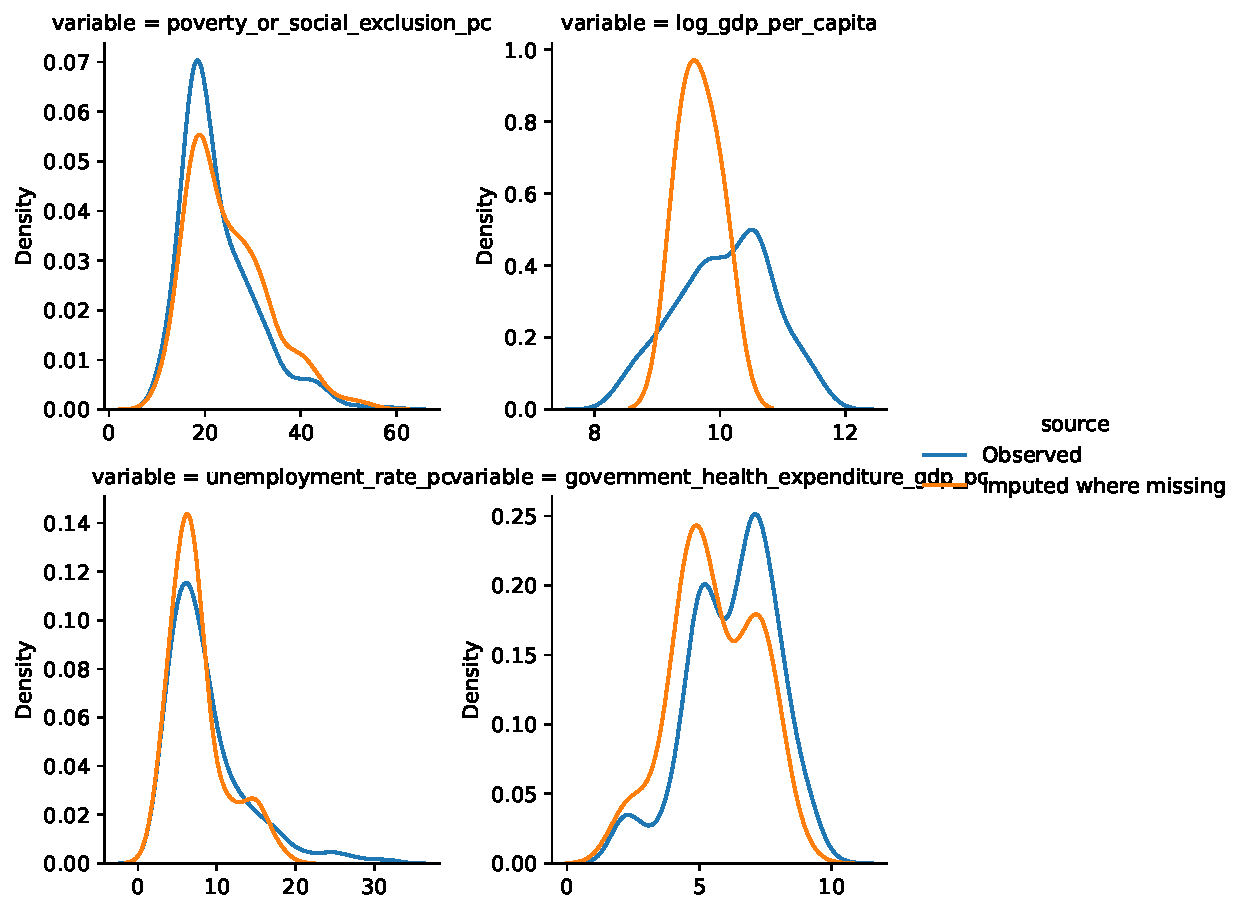
\includegraphics[width=0.86\textwidth]{mi_observed_vs_imputed_baseline}
\caption{Observed and imputed distributions in the baseline MI diagnostic. The sample is the 608-row outcome-observed target; imputed values are shown only where baseline covariates are missing.}
\label{fig:mi_observed_vs_imputed_baseline}
\vspace{0.25em}

\begin{minipage}{0.9\textwidth}
\scriptsize \textit{Source:} Author's baseline PMM imputation diagnostics. The figure checks distributional plausibility of imputed covariates.
\end{minipage}
\end{figure}

\begin{figure}[htbp]
\centering
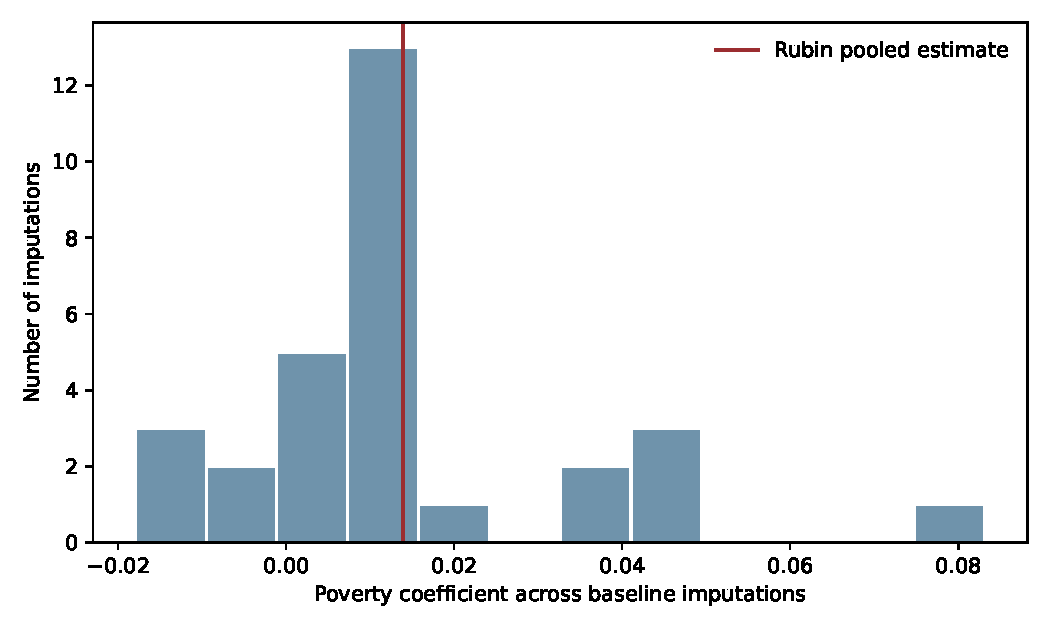
\includegraphics[width=0.72\textwidth]{mi_coefficient_distribution}
\caption{Distribution of the poverty/social-exclusion coefficient across the 30 baseline PMM imputations. The pooled estimate attenuates toward zero, but the distribution is interpreted as model-based sensitivity rather than as proof of a target-invariant coefficient.}
\label{fig:mi_coefficient_distribution}
\vspace{0.25em}

\begin{minipage}{0.86\textwidth}
\scriptsize \textit{Source:} Author's baseline PMM MI estimates. The figure shows between-imputation coefficient variation before Rubin pooling.
\end{minipage}
\end{figure}

The PMM variants expose model dependence. Baseline, no-outcome, and lagged-predictor variants attenuate the poverty coefficient toward zero, while the country-indicator variant is more positive. That pattern is not hidden: it is evidence that the imputed estimand depends on the imputation structure.

\section{MNAR Multiple Imputation}

MAR assumptions cannot be verified in Eurostat covariate coverage. Table~\ref{tab:mnar_sensitivity_results} therefore applies MNAR delta shifts only to originally missing values after the baseline PMM imputation. Poverty, GDP, and unemployment shifts are not corrected estimates. They are stress tests for whether the MAR attenuation is mechanically dependent on one favorable imputation model.

The MI attenuation is interpreted as model-based instability under a broader target population. It may reflect target-population sensitivity, imputation-model dependence, MAR violations, or structural Eurostat non-coverage. The imputation model itself is part of the sensitivity design. The MI estimates are not treated as corrected estimates. They test whether the complete-case poverty coefficient is stable under broader model-based targets; it is not.

\begin{table}[H]
\centering
\scriptsize
\caption{MNAR delta-shift sensitivity for the poverty coefficient. Scenarios shift only originally missing values after PMM imputation and are stress tests for MAR departures, not corrected estimates.}
\label{tab:mnar_sensitivity_results}
\resizebox{\textwidth}{!}{%
\begin{tabular}{@{}lrrrl@{}}
\toprule
Scenario & Coef. [95\% CI] & p-value & \(M\) & Interpretation \\
\midrule
GDP -10\% & 0.011 [-0.085, 0.107] & 0.823 & 30 & MNAR stress test \\
GDP -20\% & 0.012 [-0.085, 0.108] & 0.811 & 30 & MNAR stress test \\
GDP -5\% & 0.011 [-0.086, 0.107] & 0.828 & 30 & MNAR stress test \\
Optimistic combo & 0.010 [-0.086, 0.106] & 0.837 & 30 & MNAR stress test \\
Pessimistic combo & 0.010 [-0.086, 0.107] & 0.831 & 30 & MNAR stress test \\
Poverty +10 pp & 0.007 [-0.089, 0.103] & 0.890 & 30 & MNAR stress test \\
Poverty +2 pp & 0.010 [-0.086, 0.107] & 0.834 & 30 & MNAR stress test \\
Poverty +5 pp & 0.010 [-0.086, 0.106] & 0.845 & 30 & MNAR stress test \\
Unemployment +2 pp & 0.011 [-0.085, 0.107] & 0.827 & 30 & MNAR stress test \\
Unemployment +5 pp & 0.011 [-0.084, 0.107] & 0.817 & 30 & MNAR stress test \\
\bottomrule
\end{tabular}%
}

\vspace{0.2em}
\begin{minipage}{0.96\textwidth}\scriptsize Notes: MNAR scenarios apply documented shifts only to originally missing values after the PMM MAR imputation. They are stress tests for model dependence and should not be read as corrected estimates.\end{minipage}

\vspace{0.25em}

\begin{minipage}{0.96\textwidth}
\scriptsize \textit{Source:} Author's MNAR delta-shift sensitivity analysis. Shifts are applied only to cells originally missing before imputation.
\end{minipage}
\end{table}

\begin{table}[H]
\centering
\small
\caption{MNAR tipping-point grid for the poverty/social-exclusion coefficient. Shifts are applied only to originally missing poverty/social-exclusion values after PMM imputation and are compared with the selected complete-case FE coefficient.}
\label{tab:mnar_tipping_point_results}
\begin{tabular}{@{}lrrrl@{}}
\toprule
Poverty shift & Coef. [95\% CI] & Distance & p-value & Status \\
\midrule
-10 pp & 0.019 [-0.077, 0.116] & 0.158 & 0.697 & grid point \\
-5 pp & 0.019 [-0.077, 0.116] & 0.158 & 0.697 & grid point \\
0 pp & 0.019 [-0.077, 0.116] & 0.158 & 0.697 & grid point \\
2 pp & 0.019 [-0.077, 0.115] & 0.158 & 0.699 & grid point \\
5 pp & 0.018 [-0.078, 0.114] & 0.159 & 0.712 & grid point \\
10 pp & 0.015 [-0.080, 0.110] & 0.162 & 0.756 & grid point \\
15 pp & 0.008 [-0.085, 0.102] & 0.169 & 0.865 & grid point \\
20 pp & -0.014 [-0.108, 0.081] & 0.191 & 0.779 & grid point \\
25 pp & -0.061 [-0.165, 0.042] & 0.239 & 0.246 & grid point \\
30 pp & -0.126 [-0.239, -0.013] & 0.303 & 0.029 & grid point \\
40 pp & -0.206 [-0.325, -0.087] & 0.384 & <0.001 & grid point \\
\bottomrule
\end{tabular}

\vspace{0.2em}
\begin{minipage}{0.92\textwidth}\scriptsize Notes: Shifts are applied only to originally missing poverty/social-exclusion cells after PMM imputation. The complete-case target coefficient is 0.178. Tipping-point status: not reached within grid; estimated shift: not reached within the grid.\end{minipage}

\vspace{0.25em}

\begin{minipage}{0.92\textwidth}
\scriptsize \textit{Source:} Author's MNAR tipping-point analysis. The table asks how far missing poverty/social-exclusion values would need to be shifted to approach the selected complete-case coefficient.
\end{minipage}
\end{table}

\begin{figure}[H]
\centering
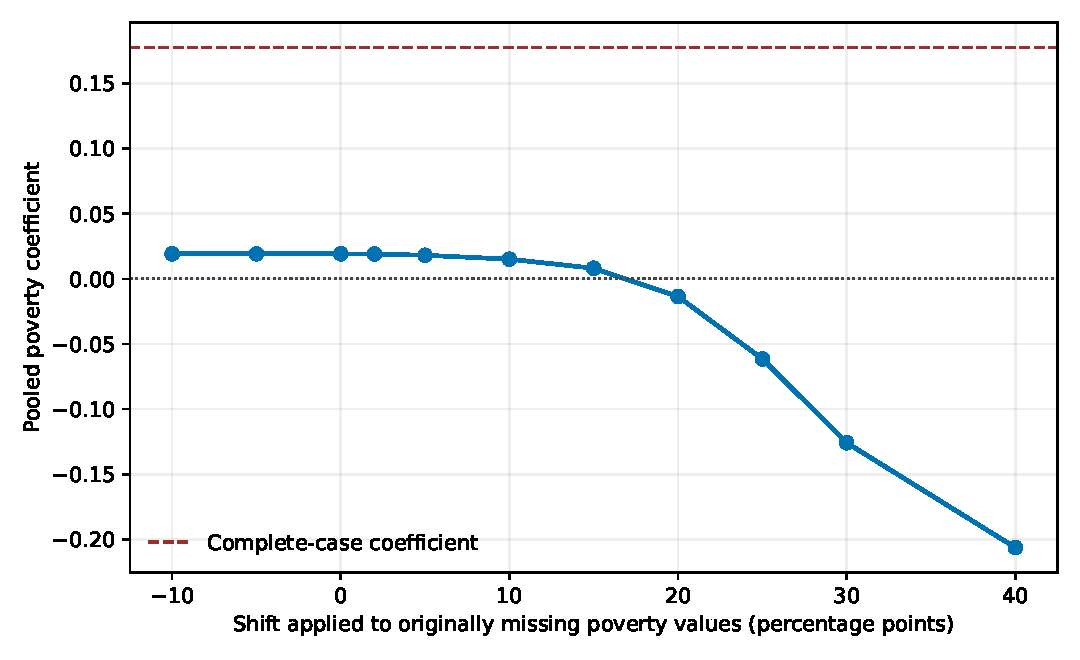
\includegraphics[width=0.78\textwidth]{mnar_tipping_point_curve}
\caption{MNAR tipping-point curve for the poverty/social-exclusion coefficient. The horizontal dashed line is the selected complete-case FE coefficient; the curve shows pooled MI coefficients after shifting originally missing poverty/social-exclusion values.}
\label{fig:mnar_tipping_point_curve}
\vspace{0.25em}

\begin{minipage}{0.86\textwidth}
\scriptsize \textit{Source:} Author's MNAR tipping-point analysis. The curve visualizes imputation-model dependence under explicit departures from MAR.
\end{minipage}
\end{figure}

\FloatBarrier

\section{Interpretation}

The regression conclusion is estimand dependence, not a stable poverty effect. The selected complete-case model gives a substantively plausible positive association, and several observed covariate-complete perturbations point in the same direction. But the coefficient changes with model structure, weighting, measurement-period restrictions, country trends, and especially the move from selected complete cases to model-based outcome-observed targets.

This is the thesis spine. Complete-case modelling in open Eurostat health-monitoring panels can silently move the analyst from an intended European monitoring population to a selected covariate-complete panel. The poverty coefficient is useful because it reveals that drift; it is not presented as a durable causal, policy, or individual-level finding.

\chapter{Target-Population Drift Reporting Protocol and Conclusion}
\label{ch:discussion_conclusion}

\section{Main Finding}

The thesis is a reproducible audit of target-population drift in public Eurostat unmet-care panels. Its central finding is not a single poverty/social-exclusion coefficient. The central finding is that aggregate monitoring and modelling conclusions change when the analyst changes indicator definition, denominator, country universe, population weighting, covariate-completeness rules, and missing-data assumptions.

The primary case remains informative because it is concrete: the observed \texttt{hlth\_silc\_08} monitoring panel has 608 country-years, while the baseline complete-case fixed-effects stress-test sample has 282 rows. The multi-outcome benchmark shows that this is part of a broader public-data problem. Population-denominator indicators, need-denominator indicators, medical care, dental care, and barrier-specific indicators do not all support the same analytical target.

\section{Reporting Protocol}

The protocol developed in the thesis is not a new estimator. It is a reporting discipline for aggregate public panels. Before interpreting a coefficient, the analyst should define the monitoring target, measure coverage drift, diagnose included-versus-excluded imbalance, compare estimands, stress-test missingness assumptions, and classify the evidence.

\begin{table}[H]
\centering
\scriptsize
\caption{Target-population drift reporting checklist. The protocol is a structured audit for public aggregate health-monitoring panels and does not introduce a new estimator.}
\label{tab:target_population_drift_reporting_checklist}
\begin{tabular}{p{0.18\linewidth}p{0.39\linewidth}p{0.33\linewidth}}
\toprule
Protocol item & Required report & Thesis output \\
\midrule
Target definition & Unit, indicator, denominator, country universe, time window, and weighting rule. & Public-data estimand registry and country-universe table. \\
Monitoring benchmark & Unweighted and population-weighted trends by indicator and universe before modelling. & Multi-outcome monitoring benchmark and coverage tables. \\
Coverage drift & Rows, countries, and years retained after each covariate or weight requirement. & Attrition matrix, retention heatmap, and primary waterfall. \\
Selection distortion & Included-versus-excluded differences in outcome, covariates, country groups, and time periods. & SMD tables, selection model, and inclusion-probability figure. \\
Estimand stability & Coefficient across complete-case, weighted, balanced, IPW, MAR MI, and MNAR sensitivity targets. & Outcome-by-estimand matrix and main sensitivity ladder. \\
Simulation stress test & Bias, sign reversal, interval coverage, and wrong-conclusion rates under controlled missingness. & Semi-synthetic missingness simulation. \\
Final label & Stable, target-dependent, denominator-dependent, missingness-dependent, imputation-model-dependent, or non-identifiable. & Final classification table. \\
\bottomrule
\end{tabular}

\end{table}

Table~\ref{tab:target_population_drift_reporting_checklist} is the reusable output of the thesis. It turns the empirical work into a sequence that another Eurostat aggregate-panel study can apply. The order matters: target definition and monitoring coverage come before regression, while coefficient interpretation comes only after the estimand matrix and simulation stress test.

\section{Failure Modes}

The thesis uses deterministic labels to avoid narrative interpretation of unstable coefficients. A result is not called stable because one table has a favourable sign. It is stable only when the main estimand families agree sufficiently on the IQR-effect scale and have enough empirical support. If the available data cannot support that standard, the result is labelled target-dependent, missingness-dependent, imputation-model-dependent, denominator-dependent, or non-identifiable.

\begin{table}[H]
\centering
\scriptsize
\caption{Failure modes in public aggregate panels. The labels classify interpretation risk after target definition, attrition, coefficient stability, and simulation diagnostics have been reported.}
\label{tab:failure_modes_public_aggregate_panels}
\begin{tabular}{p{0.19\linewidth}p{0.39\linewidth}p{0.32\linewidth}}
\toprule
Mode & Definition & Interpretation \\
\midrule
Stable & Core estimand families agree in direction and IQR-scale magnitude. & A cautious aggregate coefficient interpretation is supportable. \\
Target-dependent & Observed-data estimates change materially under weighting, balanced coverage, or country-universe restriction. & The coefficient is a property of a defined target, not of Europe in general. \\
Denominator-dependent & Population-denominator and need-denominator indicators support different interpretations. & The monitoring question must be restated before comparing coefficients. \\
Missingness-dependent & Complete-case, IPW, MAR MI, or MNAR targets materially disagree. & Covariate coverage and missing-data assumptions carry the empirical conclusion. \\
Imputation-model-dependent & MI variants disagree strongly with each other. & The imputed estimate is a model-dependent sensitivity result. \\
Non-identifiable & Too few reliable estimand families are feasible, or estimands conflict too strongly. & The public aggregate data do not support a coefficient interpretation. \\
\bottomrule
\end{tabular}

\end{table}

These labels are conservative by design. They protect the thesis from treating a selected complete-case coefficient as a general statement about European access barriers. They also prevent imputation from being misread as correction: MI and MNAR analyses are sensitivity designs, and their results remain model-dependent.

\section{Final Classification of Findings}

\begin{table}[H]
\centering
\scriptsize
\caption{Final classification of Eurostat unmet-care findings. Labels are generated from the outcome-by-estimand matrix and deterministic rules; they summarize whether a poverty/social-exclusion coefficient can be interpreted for each outcome target.}
\label{tab:final_classification_eurostat_findings}
\begin{tabular}{p{0.22\linewidth}p{0.18\linewidth}p{0.20\linewidth}p{0.30\linewidth}}
\toprule
Finding & Final label & Evidence basis & Interpretation \\
\midrule
Dental need & non-identifiable & 1 estimand families estimated & Available public aggregate data do not support a coefficient interpretation. \\
Dental population & target-dependent & 5 estimand families estimated & Interpretation changes with target population, weighting, or missing-data assumptions. \\
Medical need & non-identifiable & 1 estimand families estimated & Available public aggregate data do not support a coefficient interpretation. \\
Medical population & target-dependent & 5 estimand families estimated & Interpretation changes with target population, weighting, or missing-data assumptions. \\
Medical cost & target-dependent & 5 estimand families estimated & Interpretation changes with target population, weighting, or missing-data assumptions. \\
Medical distance & target-dependent & 5 estimand families estimated & Interpretation changes with target population, weighting, or missing-data assumptions. \\
Medical waiting & stable & 5 estimand families estimated & Observed estimands are sufficiently aligned for cautious aggregate interpretation. \\
\bottomrule
\end{tabular}

\end{table}

Table~\ref{tab:final_classification_eurostat_findings} summarizes the empirical conclusion. Several population-denominator outcomes are target-dependent: the coefficient changes when the target population, weighting rule, or missing-data assumption changes. Need-denominator outcomes are non-identifiable as coefficient targets in this public aggregate setup because too few reliable observed-data estimand families are feasible. The waiting-list population indicator is the most stable in this audit, but it remains an aggregate monitoring result, not an individual-level mechanism.

\section{What the Simulation Adds}

The semi-synthetic simulation strengthens the audit logic because it creates a reference estimand before deleting covariates. It does not claim to know the coefficient for Europe. It asks a narrower question: when a complete artificial panel is available and Eurostat-style missingness is imposed, how often do complete-case FE, population-weighted FE, IPW, PMM MI, and MNAR-shift MI recover the reference estimand?

The answer is mechanism-dependent. Some missingness patterns leave complete-case FE close to the reference estimand in this panel; other patterns create sign instability, undercoverage, or large model-based imputation movement. The simulation therefore supports the reporting protocol: analysts should report not only a coefficient but also the target drift and missingness mechanism that make the coefficient interpretable or non-identifiable.

\section{Secondary Evidence}

Prediction is deliberately appendix-level evidence. The one-year-ahead benchmark shows that previous-year persistence is difficult to beat and that flexible models do not add convincing predictive value in this small aggregate panel. This supports cautious validation practice, but it is not a main thesis contribution.

Citizenship, convergence, bivariate scatterplots, and long model ladders are also supporting material. They may provide useful context, but they do not define the thesis contribution. The thesis is strongest when every result serves the target-population drift audit.

\section{Limits}

The thesis remains aggregate, associational, and public-data-based. Country-year averages cannot identify individual mechanisms, within-country inequalities, or intervention effects. Self-reported unmet care depends on perceived need, expectations, survey wording, and denominator definition. Population weighting changes the estimand from average country to average resident; it does not automatically improve the estimate. Complete-case, IPW, MAR MI, and MNAR analyses each require assumptions that are only partly testable from public aggregate data.

The main limitation is also the reason the thesis is useful: public monitoring panels are incomplete, and incompleteness changes interpretation. The thesis does not remove that problem. It makes the problem visible and reportable.

\section{Conclusion}

This thesis formalizes and applies a reproducible target-population drift audit protocol for public Eurostat unmet-care panels. It builds a public-data estimand registry, compares multiple unmet-care indicators before modelling, measures complete-case drift, classifies coefficient stability across estimands, and stress-tests missingness through semi-synthetic simulation.

The final conclusion is controlled but strong. Eurostat unmet-care indicators are valuable for monitoring European health-access barriers, but aggregate coefficients cannot be interpreted until the analyst defines the target population, denominator, weighting rule, country universe, row-selection process, and missing-data assumption. In this thesis, many poverty/social-exclusion coefficients are target-dependent or non-identifiable rather than stable. That is the substantive result of the audit.


\appendix
\chapter{Predictive Benchmarks}
\label{ch:ml_extension}

\section{Purpose}

This appendix benchmarks one-year-ahead prediction using lagged country-level predictors. The task is intentionally modest because the panel is small and country structure is persistent.

\section{Persistence Baseline}

The decisive benchmark is simple persistence. Table~\ref{tab:ml_naive_baselines} shows that previous-year unmet need has the lowest held-out test MAE among the naive and statistical baselines and beats the flexible models in Table~\ref{tab:ml_model_performance_full}.

\begin{table}[H]
\centering
\small
\caption{Naive and statistical baselines for one-year-ahead prediction. The held-out test set is the time-ordered 2021--2023 complete-case prediction sample; predictors use prior-year country information only.}
\label{tab:ml_naive_baselines}
\begin{tabular}{@{}rrrr@{}}
\toprule
Model & MAE & RMSE & R2 \\
\midrule
Previous-year outcome & 0.587 & 1.006 & 0.850 \\
AR(1) linear & 0.661 & 1.101 & 0.820 \\
Ridge with lagged predictors & 0.695 & 1.115 & 0.816 \\
Last observed country value & 0.718 & 1.187 & 0.791 \\
Rolling country mean & 0.796 & 1.357 & 0.727 \\
Country mean & 0.855 & 1.340 & 0.734 \\
Last training-year mean & 1.815 & 2.613 & -0.013 \\
Global mean & 1.885 & 2.596 & -0.000 \\
\bottomrule
\end{tabular}

\end{table}

\begin{table}[H]
\centering
\small
\caption{Linear and flexible benchmark performance with lagged predictors. Models are trained on the pre-test complete-case prediction panel and evaluated on the same 2021--2023 held-out test years as the naive baselines. Additional model-inspection tools are not used because the chapter is a negative benchmark, not an algorithmic contribution.}
\label{tab:ml_model_performance_full}
\begin{tabular}{@{}rrrrrrr@{}}
\toprule
Model & Family & CV MAE & CV SD & Test MAE & RMSE & R2 \\
\midrule
Lasso & linear & 0.561 & 0.202 & 0.667 & 1.116 & 0.815 \\
Elastic Net & linear & 0.556 & 0.169 & 0.675 & 1.133 & 0.809 \\
Ridge & linear & 0.572 & 0.159 & 0.693 & 1.139 & 0.807 \\
Random Forest & tree & 0.544 & 0.100 & 0.727 & 1.313 & 0.744 \\
XGBoost & tree & 0.624 & 0.180 & 0.769 & 1.350 & 0.730 \\
\bottomrule
\end{tabular}

\end{table}

\section{Validation Checks}

The evaluation uses temporal train/test separation, expanding-window validation, bootstrap intervals for held-out MAE, and blocked country-holdout validation. Country-holdout validation is especially important because aggregate predictors can encode persistent country identity rather than transferable structure.

\begin{table}[H]
\centering
\small
\caption{Blocked country-holdout predictive performance. Folds hold out countries rather than years to test transfer beyond persistent country structure; no population weights are applied.}
\label{tab:ml_country_holdout_summary}
\begin{tabular}{@{}rrrrr@{}}
\toprule
model & mean\_mae & sd\_mae & mean\_rmse & folds \\
\midrule
Lasso & 0.594 & 0.210 & 0.944 & 5 \\
Elastic Net & 0.621 & 0.202 & 0.969 & 5 \\
Ridge & 0.648 & 0.206 & 0.993 & 5 \\
Random Forest & 0.747 & 0.393 & 1.228 & 5 \\
XGBoost & 0.783 & 0.330 & 1.298 & 5 \\
\bottomrule
\end{tabular}

\end{table}

\section{Interpretation}

Open Eurostat indicators contain next-year predictive signal, but simple persistence is the strongest benchmark in the held-out test. Flexible machine learning therefore remains appendix-level validation evidence rather than an independent thesis contribution.

\chapter{Appendix}
\label{ch:appendix}
\raggedbottom

\section{Regression Diagnostics}

This appendix reports only supporting material that is useful for checking the main analysis without repeating the figures already discussed in the thesis chapters. Table~\ref{tab:appendix_full_pooled_regression} gives the full pooled baseline regression, including the year indicators omitted from the compact main table. The omitted year is 2015.

\begin{table}[H]
\centering
\scriptsize
\caption{Full pooled baseline regression with year indicators}
\label{tab:appendix_full_pooled_regression}
\begin{tabular}{@{}lrrrr@{}}
\toprule
Variable & Estimate & Std. error & \(t\) & \(p\) \\
\midrule
Intercept & 7.390 & 6.813 & 1.085 & 0.278 \\
Year 2016 & -0.033 & 0.241 & -0.135 & 0.892 \\
Year 2017 & -0.428 & 0.416 & -1.028 & 0.304 \\
Year 2018 & 0.000 & 0.492 & 0.000 & 1.000 \\
Year 2019 & 0.025 & 0.559 & 0.046 & 0.964 \\
Year 2020 & -0.136 & 0.470 & -0.289 & 0.772 \\
Year 2021 & -0.171 & 0.553 & -0.308 & 0.758 \\
Year 2022 & 0.242 & 0.733 & 0.330 & 0.742 \\
Year 2023 & 0.804 & 0.772 & 1.042 & 0.297 \\
Year 2024 & 0.803 & 0.630 & 1.274 & 0.203 \\
Log GDP per capita & -0.546 & 0.593 & -0.920 & 0.358 \\
Unemployment rate & 0.160 & 0.186 & 0.861 & 0.389 \\
Poverty or social exclusion & 0.062 & 0.065 & 0.955 & 0.340 \\
Government health expenditure & 0.159 & 0.190 & 0.835 & 0.404 \\
Compulsory health financing & -0.401 & 0.243 & -1.652 & 0.099 \\
\bottomrule
\end{tabular}
\par\vspace{0.3em}
\begin{minipage}{0.96\textwidth}
\footnotesize Notes: This is the full pooled baseline specification corresponding to Table~\ref{tab:regression_main_results}, including all year-indicator coefficients. The omitted year is 2015. Standard errors are country-clustered; exact p-values are shown instead of significance stars.
\end{minipage}

\end{table}

Table~\ref{tab:appendix_regression_vif_diagnostics} reports variance inflation factors for the baseline covariates. The diagnostics are included to document the degree of collinearity among the main regressors used in the complete-case model.

\begin{table}[H]
\centering
\small
\caption{Variance inflation factors for baseline covariates}
\label{tab:appendix_regression_vif_diagnostics}
\begin{tabular}{@{}lr@{}}
\toprule
Covariate & VIF \\
\midrule
Log GDP per capita & 1.92 \\
Unemployment rate & 1.28 \\
Poverty or social exclusion & 2.00 \\
Government health expenditure & 2.31 \\
Compulsory health financing & 2.82 \\
\bottomrule
\end{tabular}
\par\vspace{0.3em}
\begin{minipage}{0.86\textwidth}
\footnotesize Notes: VIF is the variance inflation factor calculated for the five baseline covariates in the complete-case pooled regression sample. Values above 10 are commonly treated as indicating serious multicollinearity.
\end{minipage}

\end{table}

\section{Missingness and Prediction Sensitivities}

Table~\ref{tab:appendix_mi_variant_summary} documents the PMM multiple-imputation variants used to assess whether the main attenuation pattern depends on including the outcome, country-structure representation, lagged predictors, or the number of imputations.

\begin{table}[H]
\centering
\small
\caption{Multiple-imputation variants for the poverty coefficient}
\label{tab:appendix_mi_variant_summary}
\begin{tabular}{@{}lrrrr@{}}
\toprule
Variant & Coef. & SE & p-value & \(M\) \\
\midrule
Baseline PMM MI & 0.0139 & 0.0434 & 0.748 & 30 \\
No-outcome PMM MI & -0.0308 & 0.0492 & 0.532 & 30 \\
Country-FE PMM MI & 0.2516 & 0.0896 & 0.005 & 30 \\
Lagged-predictor PMM MI & -0.0472 & 0.0566 & 0.405 & 30 \\
50-imputation PMM check & 0.0122 & 0.0432 & 0.778 & 50 \\
\bottomrule
\end{tabular}

\end{table}

Table~\ref{tab:appendix_mnar_sensitivity_results} documents MNAR delta-shift scenarios. These scenarios shift only originally missing values after PMM imputation and are interpreted as stress tests rather than corrected estimates.

\begin{table}[H]
\centering
\scriptsize
\caption{MNAR delta-shift sensitivity for the poverty coefficient}
\label{tab:appendix_mnar_sensitivity_results}
\resizebox{\textwidth}{!}{%
\begin{tabular}{@{}lrrrl@{}}
\toprule
Scenario & Coef. [95\% CI] & p-value & \(M\) & Interpretation \\
\midrule
GDP -10\% & 0.011 [-0.085, 0.107] & 0.823 & 30 & MNAR stress test \\
GDP -20\% & 0.012 [-0.085, 0.108] & 0.811 & 30 & MNAR stress test \\
GDP -5\% & 0.011 [-0.086, 0.107] & 0.828 & 30 & MNAR stress test \\
Optimistic combo & 0.010 [-0.086, 0.106] & 0.837 & 30 & MNAR stress test \\
Pessimistic combo & 0.010 [-0.086, 0.107] & 0.831 & 30 & MNAR stress test \\
Poverty +10 pp & 0.007 [-0.089, 0.103] & 0.890 & 30 & MNAR stress test \\
Poverty +2 pp & 0.010 [-0.086, 0.107] & 0.834 & 30 & MNAR stress test \\
Poverty +5 pp & 0.010 [-0.086, 0.106] & 0.845 & 30 & MNAR stress test \\
Unemployment +2 pp & 0.011 [-0.085, 0.107] & 0.827 & 30 & MNAR stress test \\
Unemployment +5 pp & 0.011 [-0.084, 0.107] & 0.817 & 30 & MNAR stress test \\
\bottomrule
\end{tabular}%
}

\vspace{0.2em}
\begin{minipage}{0.96\textwidth}\scriptsize Notes: MNAR scenarios apply documented shifts only to originally missing values after the PMM MAR imputation. They are stress tests for model dependence and should not be read as corrected estimates.\end{minipage}

\end{table}

Table~\ref{tab:appendix_ml_naive_baselines} reports the naive prediction baselines used to decide whether flexible models add useful one-year-ahead predictive value.

\begin{table}[H]
\centering
\small
\caption{Naive prediction baselines}
\label{tab:appendix_ml_naive_baselines}
\begin{tabular}{@{}rrrr@{}}
\toprule
Model & MAE & RMSE & R2 \\
\midrule
Previous-year outcome & 0.587 & 1.006 & 0.850 \\
AR(1) linear & 0.661 & 1.101 & 0.820 \\
Ridge with lagged predictors & 0.695 & 1.115 & 0.816 \\
Last observed country value & 0.718 & 1.187 & 0.791 \\
Rolling country mean & 0.796 & 1.357 & 0.727 \\
Country mean & 0.855 & 1.340 & 0.734 \\
Last training-year mean & 1.815 & 2.613 & -0.013 \\
Global mean & 1.885 & 2.596 & -0.000 \\
\bottomrule
\end{tabular}

\end{table}

\section{Data Sources and Reproducibility}

Table~\ref{tab:appendix_eurostat_sources} lists the Eurostat tables and filters used to construct the datasets. The primary outcome is hlth\_silc\_08, while hlth\_silc\_08b is used only as the robustness outcome because its denominator differs from the main population-level indicator.

\begin{table}[H]
\centering
\scriptsize
\caption{Eurostat source tables, filters, and extraction dates}
\label{tab:appendix_eurostat_sources}
\resizebox{\textwidth}{!}{%
\begin{tabular}{@{}>{\raggedright\arraybackslash}p{0.15\textwidth}>{\raggedright\arraybackslash}p{0.23\textwidth}>{\raggedright\arraybackslash}p{0.45\textwidth}r@{}}
\toprule
Code & Use & Filters & Accessed \\
\midrule
\texttt{hlth\_silc\_08} & Medical population denominator & unit=PC; quantile=TOTAL; reason=TXP\_TFAR\_WLIST; age=Y\_GE16; sex=T; years 2008--2025 & 2026-06-23 \\
\texttt{hlth\_silc\_08b} & Medical need denominator & unit=PC; rskpovth=TOTAL; reason=TXP\_TFAR\_WLIST; age=Y\_GE16; sex=T; years 2021--2025 & 2026-06-23 \\
\texttt{hlth\_silc\_09} & Dental population denominator & unit=PC; quantile=TOTAL; reason=TXP\_TFAR\_WLIST; age=Y\_GE16; sex=T; years 2008--2025 & 2026-06-23 \\
\texttt{hlth\_silc\_09b} & Dental need denominator & unit=PC; rskpovth=TOTAL; reason=TXP\_TFAR\_WLIST; age=Y\_GE16; sex=T; years 2021--2025 & 2026-06-23 \\
\texttt{demo\_pjan} & Population weights & freq=A; unit=NR; age=TOTAL; sex=T; years 2008--2025 & 2026-05-21 \\
\texttt{nama\_10\_pc} & GDP per capita & unit=CP\_EUR\_HAB; na\_item=B1GQ; years 2008--2025 & 2026-05-14 \\
\texttt{une\_rt\_a} & Unemployment rate & unit=PC\_ACT; sex=T; age=Y15-74; years 2008--2025 & 2026-05-14 \\
\texttt{ilc\_peps01n} & Poverty or social exclusion & unit=PC; sex=T; age=TOTAL; years 2008--2025 & 2026-05-14 \\
\texttt{gov\_10a\_exp} & Government health expenditure & unit=PC\_GDP; sector=S13; cofog99=GF07; na\_item=TE; years 2008--2025 & 2026-05-14 \\
\texttt{hlth\_sha11\_hf} & Compulsory health financing & unit=PC\_GDP; icha11\_hf=HF1; years 2008--2025 & 2026-05-14 \\
\texttt{hlth\_sha11\_hf} & Out-of-pocket spending & unit=PC\_CHE; icha11\_hf=HF3; years 2008--2025 & 2026-05-14 \\
\texttt{hlth\_rs\_prs2} & Physicians per 100,000 & unit=P\_HTHAB; wstatus=PRACT; med\_spec=PHYS; years 2008--2025 & 2026-05-14 \\
\texttt{hlth\_rs\_bds1} & Hospital beds per 100,000 & unit=P\_HTHAB; facility=HBEDT; hlthcare=TOTAL; years 2008--2025 & 2026-05-14 \\
\texttt{ilc\_di12} & Gini coefficient & age=TOTAL; statinfo=GINI\_HND; years 2008--2025 & 2026-05-14 \\
\texttt{une\_ltu\_a} & Long-term unemployment & indic\_em=LTU; age=Y15-74; sex=T; unit=PC\_ACT; years 2008--2025 & 2026-05-14 \\
\bottomrule
\end{tabular}%
}

\end{table}

Table~\ref{tab:appendix_software_versions} records the main software environment used for data processing, modelling, and figure generation.

\begin{table}[H]
\centering
\small
\caption{Python and library versions}
\label{tab:appendix_software_versions}
\begin{tabular}{@{}ll@{}}
\toprule
Software & Version \\
\midrule
Python & 3.13.12 \\
pandas & 3.0.3 \\
scikit-learn & 1.7.1 \\
statsmodels & 0.14.6 \\
matplotlib & 3.10.8 \\
seaborn & 0.13.2 \\
\bottomrule
\end{tabular}

\end{table}

Table~\ref{tab:processed_data_dictionary_summary} summarises the processed data files submitted with the thesis package. The full column-level data dictionary is written to \texttt{outputs/processed\_data\_dictionary.csv}.

\begingroup
\scriptsize
\begin{longtable}{@{}>{\raggedright\arraybackslash}p{0.31\textwidth}rr>{\raggedright\arraybackslash}p{0.33\textwidth}@{}}
\caption{Processed data dictionary summary}\label{tab:processed_data_dictionary_summary}\\
\toprule
File & Rows & Columns & Key columns \\
\midrule
\endfirsthead
\toprule
File & Rows & Columns & Key columns \\
\midrule
\endhead
citizenship.csv & 1612 & 4 & ctry, year, unmet \\
outcome.csv & 608 & 4 & geo, year, unmet \\
outcome\_08b.csv & 154 & 4 & geo, year \\
gini.csv & 410 & 3 & geo, year \\
beds.csv & 570 & 3 & geo, year \\
lt\_unemp.csv & 572 & 3 & geo, year \\
oop\_share.csv & 475 & 3 & geo, year \\
physicians.csv & 459 & 3 & geo, year \\
population.csv & 796 & 4 & geo, year, pop \\
ml\_5a.csv & 230 & 22 & geo, year, unmet \\
ml\_5a\_splits.csv & 230 & 23 & geo, year, unmet \\
ml\_time.csv & 236 & 15 & geo, year, unmet \\
multi\_outcome\_unmet... & 2740 & 11 & geo, year \\
panel.csv & 608 & 25 & geo, year, unmet, pop \\
imp\_1.csv & 608 & 25 & geo, year, unmet, pop \\
imp\_10.csv & 608 & 25 & geo, year, unmet, pop \\
imp\_2.csv & 608 & 25 & geo, year, unmet, pop \\
imp\_3.csv & 608 & 25 & geo, year, unmet, pop \\
imp\_4.csv & 608 & 25 & geo, year, unmet, pop \\
imp\_5.csv & 608 & 25 & geo, year, unmet, pop \\
imp\_6.csv & 608 & 25 & geo, year, unmet, pop \\
imp\_7.csv & 608 & 25 & geo, year, unmet, pop \\
imp\_8.csv & 608 & 25 & geo, year, unmet, pop \\
imp\_9.csv & 608 & 25 & geo, year, unmet, pop \\
skeleton.csv & 608 & 9 & geo, year, unmet \\
controls.csv & 667 & 7 & geo, year \\
\bottomrule
\end{longtable}
\endgroup


Table~\ref{tab:output_generation_map} gives a compact map from generated thesis tables and figures to their scripts and main inputs. Full paths and exact source filenames are written to \texttt{outputs/table\_figure\_generation\_map.csv}.

\begingroup
\tiny
\begin{longtable}{@{}p{0.11\textwidth}p{0.39\textwidth}p{0.13\textwidth}p{0.11\textwidth}@{}}
\caption{Table and figure generation map}\label{tab:output_generation_map}\\
\toprule
Use & Output & Script & Input \\
\midrule
\endfirsthead
\toprule
Use & Output & Script & Input \\
\midrule
\endhead
App. & 08b\_minus\_08\_differen... & extra & C/08b \\
App. & 08b\_vs\_08\_scatter.pdf & extra & C/08b \\
App. & citizenship\_gap\_corre... & extra & C/08b \\
App. & citizenship\_unmet\_nee... & extra & C/08b \\
App. & citizenship\_unmet\_nee... & extra & C/08b \\
App. & citizenship\_unmet\_nee... & extra & C/08b \\
Ch. 4 & complete\_case\_attriti... & full & Panel \\
Ch. 2 & conceptual\_selection\_... & diagram & Concept \\
App. & convergence\_sigma.pdf & extra & C/08b \\
Ch. 4 & descriptive\_country\_r... & full & Panel \\
App. & descriptive\_country\_r... & full & Panel \\
Ch. 4 & descriptive\_country\_y... & full & Panel \\
Ch. 4 & descriptive\_estimand\_... & full & Panel \\
App. & descriptive\_eu\_trend.pdf & full & Panel \\
App. & descriptive\_trend\_eur... & full & Panel \\
App. & descriptive\_trend\_wit... & extra & C/08b \\
App. & leave\_one\_country\_out... & missing & Panel \\
App. & leave\_one\_year\_out\_po... & missing & Panel \\
Ch. 5 & mi\_coefficient\_distri... & missing & Panel \\
App. & mi\_imputed\_share\_heat... & missing & Panel \\
App. & mi\_imputed\_share\_heat... & missing & Panel \\
App. & mi\_imputed\_share\_heat... & missing & Panel \\
App. & mi\_imputed\_share\_heat... & missing & Panel \\
App. & mi\_imputed\_share\_heat... & missing & Panel \\
App. & mi\_imputed\_share\_heat... & missing & Panel \\
App. & mi\_imputed\_share\_heat... & missing & Panel \\
App. & mi\_imputed\_share\_heat... & missing & Panel \\
App. & mi\_imputed\_share\_heat... & missing & Panel \\
Ch. 5 & mi\_observed\_vs\_impute... & missing & Panel \\
App. & mi\_observed\_vs\_impute... & missing & Panel \\
App. & mi\_observed\_vs\_impute... & missing & Panel \\
App. & mi\_observed\_vs\_impute... & missing & Panel \\
App. & mi\_observed\_vs\_impute... & missing & Panel \\
App. & mi\_observed\_vs\_impute... & missing & Panel \\
App. & mi\_observed\_vs\_impute... & missing & Panel \\
App. & mi\_observed\_vs\_impute... & missing & Panel \\
App. & mi\_observed\_vs\_impute... & missing & Panel \\
Ch. 3; Ch. 4 & missingness\_heatmap.pdf & full & Panel \\
App. & missingness\_heatmap\_c... & full & Panel \\
Ch. 3; Ch. 4 & missingness\_heatmap\_f... & full & Panel \\
App. & missingness\_heatmap\_o... & full & Panel \\
App. & missingness\_heatmap\_p... & full & Panel \\
Ch. 3; Ch. 4 & missingness\_heatmap\_s... & full & Panel \\
Ch. 5 & missingness\_inclusion... & full & Panel \\
App. & ml\_actual\_vs\_predicte... & ml & ML \\
App. & ml\_actual\_vs\_predicte... & ml & ML \\
App. & ml\_actual\_vs\_predicte... & ml & ML \\
App. & ml\_calibration\_plot.pdf & ml & ML \\
App. & ml\_expanding\_window\_v... & ml & ML \\
App. & ml\_importance\_compari... & ml & ML \\
App. & ml\_importance\_stabili... & ml & ML \\
App. & ml\_learning\_curves.pdf & ml & ML \\
App. & ml\_permutation\_vs\_imp... & ml & ML \\
App. & ml\_residuals\_by\_count... & ml & ML \\
App. & ml\_residuals\_by\_count... & ml & ML \\
App. & ml\_residuals\_by\_count... & ml & ML \\
App. & ml\_residuals\_vs\_predi... & ml & ML \\
App. & ml\_residuals\_vs\_predi... & ml & ML \\
App. & ml\_residuals\_vs\_predi... & ml & ML \\
App. & ml\_tree\_feature\_impor... & ml & ML \\
App. & ml\_validation\_tuning\_... & ml & ML \\
Ch. 5 & mnar\_tipping\_point\_cu... & missing & Panel \\
App. & model\_correlations\_he... & full & Panel \\
Ch. 5 & model\_ladder\_coeffici... & full & Panel \\
Ch. 4 & multi\_outcome\_monitor... & full & Panel \\
Ch. 5 & multi\_outcome\_primary... & full & Panel \\
Ch. 5 & multi\_outcome\_retenti... & full & Panel \\
Ch. 5 & outcome\_estimand\_coef... & full & Panel \\
App. & outcome\_missingness\_h... & full & Panel \\
App. & panel\_correlations\_he... & full & Panel \\
App. & panel\_heterogeneity.pdf & full & Panel \\
App. & panel\_variable\_distri... & full & Panel \\
Ch. 3 & population\_weighted\_t... & full & Panel \\
App. & poverty\_robustness\_fo... & missing & Panel \\
App. & regression\_fe\_coeffic... & missing & Panel \\
App. & regression\_robustness... & full & Panel \\
App. & scatter\_unmet\_vs\_comp... & full & Panel \\
App. & scatter\_unmet\_vs\_gdp\_... & full & Panel \\
App. & scatter\_unmet\_vs\_gini... & full & Panel \\
App. & scatter\_unmet\_vs\_gove... & full & Panel \\
App. & scatter\_unmet\_vs\_hosp... & full & Panel \\
App. & scatter\_unmet\_vs\_log\_... & full & Panel \\
App. & scatter\_unmet\_vs\_long... & full & Panel \\
App. & scatter\_unmet\_vs\_oop\_... & full & Panel \\
App. & scatter\_unmet\_vs\_phys... & full & Panel \\
App. & scatter\_unmet\_vs\_pove... & missing & Panel \\
App. & scatter\_unmet\_vs\_unem... & full & Panel \\
Ch. 5 & simulation\_bias\_by\_me... & full & Panel \\
Ch. 5 & simulation\_target\_dis... & full & Panel \\
App. & tree\_feature\_importan... & full & Panel \\
App. & unmet\_need\_trends\_all... & full & Panel \\
App. & unmet\_need\_vs\_gdp\_per... & full & Panel \\
App. & unmet\_need\_vs\_poverty... & missing & Panel \\
App. & unmet\_need\_vs\_unemplo... & full & Panel \\
App. & appendix\_full\_pooled\_... & full & Panel \\
Ch. 4 & attrition\_by\_country\_... & full & Panel \\
Ch. 4 & attrition\_by\_country\_... & full & Panel \\
Ch. 4 & attrition\_by\_covariat... & full & Panel \\
App. & attrition\_by\_year.tex & full & Panel \\
App. & citizenship\_gap\_clust... & extra & C/08b \\
App. & citizenship\_gap\_regre... & extra & C/08b \\
App. & citizenship\_gap\_table... & extra & C/08b \\
Ch. 4 & complete\_case\_attriti... & full & Panel \\
Ch. 5 & complete\_case\_selecti... & missing & Panel \\
App. & country\_coverage.tex & full & Panel \\
Ch. 3 & country\_universe.tex & missing & Panel \\
App. & descriptive\_statistic... & full & Panel \\
Ch. 5 & estimand\_framework.tex & missing & Panel \\
App. & eurostat\_sources\_appe... & summary & Gen. \\
Ch. 7 & failure\_modes\_public\_... & full & Panel \\
Ch. 5 & fe\_fit\_diagnostics.tex & missing & Panel \\
Ch. 5 & fe\_inference\_comparis... & missing & Panel \\
Ch. 7 & final\_classification\_... & full & Panel \\
Ch. 4 & included\_vs\_excluded\_... & full & Panel \\
Ch. 4 & leave\_one\_variable\_ou... & missing & Panel \\
Ch. 5 & main\_sensitivity\_ladd... & missing & Panel \\
Ch. 5 & mi\_diagnostics\_summar... & missing & Panel \\
Ch. 5 & mi\_pmm\_donor\_diagnost... & missing & Panel \\
App.; Ch. 5 & mi\_variant\_summary.tex & missing & Panel \\
Ch. 3; Ch. 4 & missingness\_compariso... & full & Panel \\
Ch. 5 & missingness\_robustnes... & missing & Panel \\
Ch. 6 & ml\_country\_holdout\_su... & ml & ML \\
App. & ml\_hyperparameter\_gri... & ml & ML \\
Ch. 6 & ml\_model\_performance\_... & ml & ML \\
App.; Ch. 6 & ml\_naive\_baselines.tex & ml & ML \\
App. & ml\_paired\_tree\_mae\_di... & ml & ML \\
App. & ml\_test\_mae\_bootstrap... & ml & ML \\
App. & ml\_time\_aware\_fold\_re... & ml & ML \\
App.; Ch. 5 & mnar\_sensitivity\_resu... & missing & Panel \\
Ch. 5 & mnar\_tipping\_point\_re... & missing & Panel \\
Ch. 5 & model\_ladder\_results.tex & full & Panel \\
Ch. 5 & multi\_outcome\_attriti... & full & Panel \\
App. & multi\_outcome\_country... & full & Panel \\
Ch. 4 & multi\_outcome\_coverag... & full & Panel \\
Ch. 5 & multi\_outcome\_include... & full & Panel \\
Ch. 4 & multi\_outcome\_monitor... & full & Panel \\
Ch. 5 & multi\_outcome\_primary... & full & Panel \\
App. & multiple\_imputation\_s... & full & Panel \\
Ch. 5 & outcome\_estimand\_coef... & full & Panel \\
Ch. 5 & outcome\_failure\_class... & full & Panel \\
App. & output\_generation\_map... & summary & Gen. \\
App. & poverty\_robustness\_su... & missing & Panel \\
App. & processed\_data\_dictio... & summary & Gen. \\
Ch. 3; Ch. 4 & public\_data\_estimand\_... & full & Panel \\
App. & reduced\_covariate\_sen... & full & Panel \\
App. & regression\_country\_gr... & full & Panel \\
App. & regression\_crisis\_exc... & full & Panel \\
App. & regression\_lag\_robust... & full & Panel \\
Ch. 5 & regression\_main\_resul... & full & Panel \\
App. & regression\_multilevel... & full & Panel \\
App. & regression\_robustness... & full & Panel \\
App. & regression\_sensitivit... & full & Panel \\
App. & regression\_sensitivit... & full & Panel \\
App. & regression\_vif.tex & full & Panel \\
App. & regression\_vif\_diagno... & full & Panel \\
Ch. 3 & robustness\_08b\_result... & extra & C/08b \\
App. & simulation\_complete\_c... & full & Panel \\
Ch. 5 & simulation\_main\_summa... & full & Panel \\
App. & software\_versions.tex & summary & Gen. \\
Ch. 7 & target\_population\_dri... & missing & Panel \\
Ch. 5 & target\_population\_sen... & missing & Panel \\
Ch. 5 & universe\_sensitivity\_... & full & Panel \\
Ch. 3 & variable\_summary.tex & full & Panel \\
\bottomrule
\end{longtable}
\endgroup


The computational workflow is fully scripted in the local project directory. Raw Eurostat JSON downloads are stored in \texttt{data/raw}; processed country-year files are stored in \texttt{data/processed}; generated CSV diagnostics are stored in \texttt{outputs}; generated LaTeX tables are stored in \texttt{tables}; and generated figures are stored in \texttt{figures}. The command order is:
\begin{verbatim}
rtk python src/run_full_thesis_analysis.py
rtk python src/generate_conceptual_selection_diagram.py
rtk python src/run_missingness_robustness.py
rtk python src/run_step5_ml_analysis.py
rtk python src/run_step6_additional_analysis.py
rtk python src/run_step7_master_summary.py
\end{verbatim}
The raw-data download workflow is part of the first command: it calls the Eurostat API for the main outcome, robustness outcome, citizenship table, population weights, and control/feature covariates using the filters listed in Table~\ref{tab:appendix_eurostat_sources}. The main table and figure generation map is:
\begin{itemize}
    \item Step 1 builds the panel, descriptive figures, baseline regressions, population-weighted trends, and source register;
    \item the diagram script creates the conceptual selection and estimand figure;
    \item the missingness script creates target-population sensitivity, IPW, MI, and poverty-robustness outputs;
    \item the prediction script creates one-year-ahead baselines, reduced benchmark-model comparisons, and country-holdout validation;
    \item the additional-analysis script creates citizenship paired-gap checks and \texttt{hlth\_silc\_08b} denominator robustness;
    \item the summary script creates the manifest, software versions, command order, hashes, and output checks.
\end{itemize}
All stochastic analyses use random seed 42 unless explicitly stated otherwise. The reproducibility manifest records Python and package versions, input and script hashes, output hashes, command order, the population-weighting source, and the machine-learning hyperparameter grids. The submitted package also includes raw-download instructions, an output hash manifest, and a reproducibility archive under \texttt{outputs}. The thesis does not cite a public code repository; reproducibility is documented through the submitted local scripts, raw downloads, processed files, generated outputs, source register, and manifest.


\printbibliography

\end{document}
